%%%%%%%%%%%%%%%%%%%%%%%%%%%%%%%%%%%%%%%%%%%%%%%%%%%%%%%%%%%%
\documentclass[a4paper,english]{report}    % list options between brackets

\RequirePackage[dvips]{color}
\RequirePackage{setspace}
\RequirePackage{floatflt,epsfig}
\RequirePackage{float}
\RequirePackage{amsfonts}
\RequirePackage{amsmath}
\RequirePackage{alltt}
\RequirePackage[sectionbib]{chapterbib}
\RequirePackage{ae}
\RequirePackage{times}
\RequirePackage{fancyheadings}

\usepackage{makeidx}  
\makeindex             

%%%%%%%%%%%%%%%%%%%%%%%%%%%%%%%%%%%%%%%%%%%%%%%%%%%%%%%%%%%%

\newcommand{\Sf}[1]{\textsf{#1}}
\newcommand{\Bf}[1]{{\sffamily\bfseries}}
\newcommand{\Bfm}[1]{\mbox{\boldmath{${#1}$}}}
\newcommand{\URL}[1]{\texttt{#1}}

% Some new commands...
\def\xwin{X Window System}
\def\xbr{Xbrowse}
\def\prag{\Tt{\#pragma}}

\newcommand{\inxgra}[2]{{\centerline{\includegraphics[width=#1]{#2}}}}
\newcommand{\inygra}[2]{{\centerline{\includegraphics[height=#1]{#2}}}}
\newcommand{\incgra}[2]{{\centerline{\includegraphics[height=#1]{#2}}}}

\providecommand{\ftn}{Fort\-ran~90}
\providecommand{\Idx}[1]{{#1}\index{#1}}

\newcommand{\ttbegin}{\begin{alltt}}
\newcommand{\ttend}{\end{alltt}}
\newcommand{\keno}{$\backslash$}
%%%%%%%%%%%%%%%% Definitions for Elmer Solver Manuals %%%%%%%%%%%%%%%%%

%\newcommand{\Vec}[1]{\mathify{\mathbf{#1}}}
%\newcommand{\Vec}[1]{\vec{#1}}
\newcommand{\Div}{\nabla\cdot}
\newcommand{\Curl}{\nabla\times}
\newcommand{\Grad}{\nabla}


\definecolor{SifCol}{rgb}{0.5,0.5,0.5}
%normal item, with text also (2 parameters + text)
\newcommand{\sifitem}[2]{\item[\tt{#1}]\hspace{1mm}{\color{SifCol}\hspace{1mm}\tt{#2}}\newline} 
%item with two fields but no text
\newcommand{\sifitemnt}[2]{\item[\tt{#1}]\hspace{1mm}{\color{SifCol}\hspace{1mm}\tt{#2}}} 
\newcommand{\sifbegin}{\begin{description}}
\newcommand{\sifend}{\end{description}}
\newcommand{\modinfo}[2]{{\bf{#1}}: {#2}\newline}

\newcommand{\Matr}[1]{\mbox{\boldmath{${#1}$}}}
\newcommand{\Der}[2]{\frac{\partial{#1}}{\partial{#2}}}
\newcommand{\Secder}[2]{\frac{\partial^2{#1}}{\partial{#2}^2}}
\newcommand{\Inv}[1] {\frac{1}{#1}}
%\DeclareMathOperator{\Div}{div}
%\DeclareMathOperator{\Grad}{grad}
%\DeclareMathOperator{\Curl}{curl}

% Use these to make the printable area bigger
% Also have the option 'ownsize' active in the documentclass
\setlength{\hoffset}{-15mm}
\setlength{\voffset}{-10mm}
\addtolength{\textwidth}{30mm}
\addtolength{\textheight}{20mm}
%\addtolength{\headwidth}{30mm}

% Make the headings fancier
\pagestyle{fancy}
\lhead[\normalfont\small\bf\thepage]{\normalfont\small\slshape\rightmark}
\rhead[\small\slshape\lefthead]{\normalfont\small\bf \thepage}
\setlength{\headrulewidth}{0.4pt}
%\renewcommand{\chaptermark}[1]{\markright{\bf \chaptername \ \thechapter.\ #1}{}}
\renewcommand{\chaptermark}[1]{\markright{\bf \thechapter.\ #1}{}}
\renewcommand{\sectionmark}[1]{}
\renewcommand{\subsectionmark}[1]{}
\cfoot{}


% This sets the Elmer version in the documentation
\newcommand{\elmerversion}{~5.4}


%\pagenumbering{arabic}

%%%%%%%%%%%%%%%%%%%%%%%%%%%%%%%%%%%%%%%%%%%%%%%%%%%%%%%%%%%%

\title{\Huge{\bf Elmer Models Manual}}
\author{CSC, the Finnish IT Center for Science}
\date{\today}

%%%%%%%%%%%%%%%%%%%%%%%%%%%%%%%%%%%%%%%%%%%%%%%%%%%%%%%%%%%%

\begin{document}
\maketitle

\chapter*{Copyrights}

This document gives practical examples of the use of Elmer,
a finite element software for multiphysical problems.
The copyright if this document and Elmer software belong to
CSC -- IT Center for Science, Finland, 1995--2008. 

Elmer program is free software; you can redistribute it and/or
modify it under the terms of the GNU General Public License
as published by the Free Software Foundation; either version 2
of the License, or (at your option) any later version.

This program is distributed in the hope that it will be useful,
but WITHOUT ANY WARRANTY; without even the implied warranty of
MERCHANTABILITY or FITNESS FOR A PARTICULAR PURPOSE.  See the
GNU General Public License for more details.

CSC assumes no responsibility or liability on any errors or inaccuracies in 
Elmer program or documentation. Any kind of material damages or other indirect
consequences resulting from any Elmer part, documentation discrepancies and 
errors or non-anticipated program behavior are limited to the value of 
appropriate products purchased from CSC. 

This document is for informational use only. All information and specifications
given have been carefully prepared by the best efforts of CSC, and are believed
to be true and accurate as of time publishing. CSC reserves the right to 
modify Elmer and its documents without notice. \\  \mbox{} \\

\textbf{Additional software product copyrights included in Elmer}

Copyright, and License:

UMFPACK Version 4.3, Jan. 16, 2004. Copyright (c) 2004 by Timothy
A. Davis, University of Florida, davis@cise.ufl.edu. All Rights
Reserved. 


UMFPACK License: 

Your use or distribution of UMFPACK or any derivative code implies
that you agree to this License. 

      THIS MATERIAL IS PROVIDED AS IS, WITH ABSOLUTELY NO WARRANTY
      EXPRESSED OR IMPLIED. ANY USE IS AT YOUR OWN RISK. 

      Permission is hereby granted to use or copy this program,
      provided that the Copyright, this License, and the Availability
      of the original version is retained on all copies. User
      documentation of any code that uses UMFPACK or any modified
      version of UMFPACK code must cite the Copyright, this License,
      the Availability note, and "Used by permission." Permission to
      modify the code and to distribute modified code is granted,
      provided the Copyright, this License, and the Availability note
      are retained, and a notice that the code was modified is
      included. This software was developed with support from the
      National Science Foundation, and is provided to you free of
      charge. 


\chapter*{About ElmerGrid Manual}

The ElmerGrid Manual is part of the documentation of 
Elmer finite element software package.
ElmerGrid Manual gives instruction 
on the usage of ElmerGrid, the mesh generation and manipulation utility of Elmer.

The present ElmerGrid Manual
corresponds to software version \elmerversion{}.
The latest versions of Elmer software and its documentation
are available at the Elmer homepage at
\URL{http://www.csc.fi/elmer}. 




%%%%%%%%%%%%%%%%%%%%%%%%%%%%%%%%%%%%%%%%%%%%%%%%%%%%%%%%%%%%

%\pagenumbering{roman}
\pagestyle{empty}

% Table of contents:
\setcounter{secnumdepth}{2}
\setcounter{tocdepth}{1}  
\tableofcontents

%%%%%%%%%%%%%%%%%%%%%%%%%%%%%%%%%%%%%%%%%%%%%%%%%%%%%%%%%%%%
% Headings and Chapter name

\renewcommand{\chaptername}{Model}
\newpage
\pagestyle{fancy}

%%%%%%%%%%%%%%%%%%%%%%%%%%%%%%%%%%%%%%%%%%%%%%%%%%%%%%%%%%%%


% Heat and Mass Transfer
\graphicspath{{./}{heatequation/}}
\chapter{Heat Equation}

\modinfo{Module name}{included in solver}
\modinfo{Module subroutines}{\Idx{HeatSolve}}
\modinfo{Module authors}{Juha Ruokolainen}
\modinfo{Document authors}{Juha Ruokolainen, Ville Savolainen}
\modinfo{Document edited}{July 29th 2002}

\section{Introduction}

Heat equation results from the requirement of \Idx{energy conservation}.
In addition the Fourier's law is used to model
the heat conduction. The linearity of the equation may be 
ruined by temperature dependent thermal conductivity, or by
heat radiation.

\section{Theory}

\subsection{Governing Equations}
The incompressible heat equation is expressed as
\begin{equation}
\rho  c_p\left( \frac{\partial T}{\partial t}+(\vec u\cdot\nabla) T\right) - 
\nabla\cdot(k\nabla T) =
\overline{\overline\tau}:\overline{\overline \varepsilon} + \rho h,
\label{heat_equation}
\end{equation}
where $\rho$ is the density, $c_p$ the heat capacity at constant pressure, 
$T$ the temperature, $\vec u$ the convection velocity, $k$ the heat 
conductivity and $h$ is source of heat.
The term $\overline{\overline\tau}:\overline{\overline \varepsilon}$ is the
frictional viscous heating, which is negligible in most cases. For Newtonian
fluids, the viscous
part of the stress tensor is
\begin{equation}
\overline{\overline\tau} = 2\mu \overline{\overline\varepsilon},
\end{equation}
where $\overline{\overline \varepsilon}$ the linearized strain rate tensor.

Eq.\ref{heat_equation} applies also for solids, setting $\vec u = 0$. For
solids, conduction may be anisotropic and the conductivity a tensor.

For compressible fluids, the heat equation is written as
\begin{equation}
\rho c_v\left(\frac{\partial T}{\partial t} + \vec{u}\cdot\nabla T\right) -
\nabla\cdot\left(k\nabla T\right) = - p \nabla\cdot\vec{u} 
+ \overline{\overline\tau}:\overline{\overline \varepsilon}
+ \rho h,
\end{equation}
where $c_v$ is the heat capacity at constant volume. The density needs to be
calculated from the equation of state, e.g., perfect gas law. More
information is given in the chapter describing the Navier-Stokes equation.

The Elmer heat equation module is capable of simulation heat transfer by
conduction, convection, and diffuse gray radiation. Also a phase change
model is included. Couplings to other modules include, convection by
fluid flow, frictional heating (modules providing flow fields), and
resistive heating (modules providing magnetic and/or electric fields).


\subsection{Phase Change Model}

Elmer has an internal fixed grid phase change model. Modelling phase change is done
by modifying the definition of heat capacity according to whether
a point in space is in solid or liquid phase or in a 'mushy' region.
The choice of heat capacity within the intervals is explained in detail
below.

This type of algorithm is only applicable, when the phase change occurs
within finite temperature interval. If the modelled material is such that
the phase change occurs within very sharp temperature interval, this
method might not be appropriate.

For the solidification phase change model Elmer uses,  we need enthalpy.
The enthalpy is defined to be
\begin{equation}
H(T) = \int_0^T \left ( \rho c_p + \rho L\frac{\partial f}{\partial \lambda}\right )d\lambda,
\end{equation}
where $f(T)$ is the fraction of solid material as a function of
temperature, and $L$ is the latent heat.
The enthalpy-temperature curve is used
to compute an effective heat capacity, whereupon the equations become identical
to the heat equation. There are two ways of computing the effective heat capacity in Elmer:
\begin{equation}
c_{p,\mathrm{eff}} = \frac{\partial H}{\partial T},
\end{equation}
and
\begin{equation}
c_{p,\mathrm{eff}} = \left ( \frac{\nabla H\cdot\nabla H}{\nabla T\cdot\nabla T}\right )^{1/2}.
\end{equation}
The former method is used only if the local temperature gradient is very small, while
the latter is the preferred method. In transient simulations a third method is used, given
by
\begin{equation}
c_{p,\mathrm{eff}} = \frac{\partial H/\partial t}{\partial T/\partial t}.
\end{equation}

\subsection{Additional Heat Sources}

Frictional heating is calculated currently, for both incompressible and 
compressible fluids, by the heat source
\begin{equation}
h_f = 2\mu\overline{\overline\varepsilon}:\overline{\overline\varepsilon}.
\end{equation}

In case there are currents in the media the also the 
the resistive heating may need to be considered.
The \Idx{Joule heating} is then given by
\begin{equation}
h_m = \frac{1}{\sigma} \vec J \cdot \vec J.
\end{equation}
In the above equations, $\vec B$ and $\vec E$ are the magnetic and electric
fields, respectively. The current density $\vec J$ is defined as
\begin{equation}
\vec J = \sigma(\vec E + \vec u\times \vec B).
\end{equation}


\subsection{Boundary Conditions}
For temperature one can apply boundary conditions and have either temperature 
or heat flux prescribed.

\Idx{Dirichlet boundary condition} (temperature is 
prescribed) reads as
\begin{equation}
T=T_b.
\end{equation}
\noindent The value  of $T_b$ can be constant or a function of time, position or 
other variables. 

Heat flux depending on heat transfer coefficient $\alpha$ and external
temperature $T_{\mathrm{ext}}$ may be written as
\begin{equation}
-k\frac{\partial T}{\partial n} =\alpha (T-T_{ext} ).
\end{equation}
Both variables $\alpha$ and $T_\mathrm{ext}$ can be constant or functions of time, 
position or other variables. If the heat transfer coefficient $\alpha$ is equal
to zero, it means that the heat flux on a boundary is identically zero. The 
\Idx{Neumann boundary condition} $-k\partial T/\partial n =0$ is also used in a 
symmetry axis in 2D, axisymmetric or cylindrical problems.

Heat flux can consist of idealized radiation whereupon
\begin{equation}
-k\frac{\partial T}{\partial n} =\sigma\varepsilon (T^4 -T^4_\mathrm{ext} ).
\label{radcondition}
\end{equation}
Above,  $\sigma$ is the \Idx{Stefan-Boltzmann constant} and $\varepsilon$ the 
surface emissivity. The emissivity and the external temperature can 
again be constant or functions of time, position, or other variables.

If the surface $k$ is receiving radiation from other surfaces in the system,
then the heat flux reads as
\begin{equation}
-k_k \frac{\partial T_k}{\partial n_k} = \sigma \varepsilon_k (T_k^4 -
{1\over {A_k \varepsilon_k}} \sum_{i=1}^N G_{ik} \varepsilon_i  T_i^4 A_i ),
\end{equation}
where the subscripts $i$ and $k$ refer to surfaces $i$ and $k$, and the parameters $A_i$ and
$A_k$ to the specific surface areas. The factors $G_{ik}$ are \Idx{Gebhardt factors}, and
$N$ represents the total number of radiating surfaces present in the system.
Emissivities are assumed to be constant on each surface.

The heat equation is nonlinear when radiation is modelled.
The nonlinear term in the boundary condition (\ref{radcondition})
can be linearized as
\begin{eqnarray}
T^4 - T^4_\mathrm{ext} \approx
( {\cal T}^3 + T_\mathrm{ext} {\cal T}^2  + T^2_\mathrm{ext} {\cal T} + 
T^3_\mathrm{ext} )( T-T_\mathrm{ext} ),
\end{eqnarray}
where $\cal{T}$ is the temperature from the previous iteration.

One may also give an additional heat flux term as
\begin{equation}
-k\frac{\partial T}{\partial n} = q.
\end{equation}

\section{Keywords} 

\sifbegin
\sifitemnt{Constants}{}
\sifbegin
\sifitem{Stefan Boltzmann}{Real}
The value of the Stefan-Boltzmann constant needed for 
thermal radiation.
\sifend

\sifitem{Simulation}{}
The simulation section gives the case control data:
\sifbegin
\sifitem{Simulation Type}{String} Heat equation may be either 
{\tt Transient} or {\tt Steady State}.
\sifitem{Coordinate System}{String} Defines the coordinate system to be used, one of:
{\tt Cartesian 1D}, {\tt Cartesian 2D},~ ~{\tt Cartesian 3D},~ ~{\tt Polar 2D},~ 
~{\tt Polar 3D},~ ~{\tt Cy\-lin\-dric},~ ~{\tt Cylindric Symmetric}~
~and~ ~{\tt Axi Symmetric}.
\sifitem {Gebhardt Factors}{File}
If the model includes diffuse gray radiation, the file containing the Gebhardt factors
must be given. This file is written by the program {\tt GebhardtFactors} as a preprocessing step.
\sifitem{View Factors}{File} 
If the model includes diffuse gray radiation, the file containing the view factors
must be given to the program computing the Gebhardt factors. 
This file is written by the program {\tt ViewFactors} as a
preprocessing step. The tasks of computing view factors and the Gebhardt 
factors have been divided, because
the view factors depend only on geometry (and thus the mesh), while the Gebhardt factors also depend on
the boundary emissivities. 
\sifitem{Timestepping Method}{String} 
Possible values of this parameter are {\tt Newmark} (an additional
parameter {\tt Newmark Beta} must be given), {\tt BDF} ({\tt BDF Order} must be given). Also as a
shortcut to {\tt Newmark}-method with values of {\tt Beta}$=0.0, 0.5,$ $1.0$ the keywords 
{\tt Explicit Euler}, {\tt Crank-Nicolson}, and {\tt Implicit Euler} may be given respectively.
The recommended choice for the first order time integration is the BDF method of order 2.
\sifitem{BDF Order}{Integer}
Value may range from 1 to 5.
\sifitem{Newmark Beta}{Real} Value in range from 0.0 to 1.0. The value 0.0 equals to
the explicit Euler integration method and the value 1.0 equals to the implicit Euler method. 
\sifend

\sifitem{Solver}{solver id}
The solver section defines equation solver control variables. Most of the possible
keywords -- related to linear algebra, for example -- are common for all the solvers and are 
explained elsewhere.
\sifbegin
\sifitem{Equation}{String Heat Equation}
The name of the equation.
\sifitem{Nonlinear System Convergence Tolerance}{Real}
The criterion to
terminate the nonlinear iteration after the relative change of the norm of the field variable
between two consecutive iterations is small enough
$$
 ||T_i-T_{i-1}|| < \epsilon ||T_i||,
$$
where $\epsilon$ is the value given with this keyword.
\sifitem{Nonlinear System Max Iterations}{Integer}
The maximum number of nonlinear iterations the
solver is allowed to do.
\sifitem{Nonlinear System Newton After Iterations}{Integer}
Change the nonlinear solver type to
Newton iteration after a number of Picard iterations have been performed. If a given
convergence tolerance between two iterations is met before the iteration count is met,
it will switch the iteration type instead. In the heat equation the Picard iterations 
means that the radiation term is factorized to linear and third-power terms.
\sifitem{Nonlinear System Newton After Tolerance}{Real}
Change the nonlinear solver type to
Newton iteration, if the relative change of the norm of the field variable meets a
tolerance criterion:
$$
 ||T_i-T_{i-1}|| < \epsilon ||T_i||,
$$
where $\epsilon$ is the value given with this keyword.
\sifitem{Nonlinear System Relaxation Factor}{Real}
Giving this keyword triggers the use
of  relaxation in the nonlinear equation solver.
Using a factor below unity is sometimes required to achieve convergence of the nonlinear system.
A factor above unity might speed up the convergence. Relaxed variable is defined as follows:
$$
 T^{'}_i = \lambda T_i + (1-\lambda) T_{i-1},
$$
where $\lambda$ is the factor given with this keyword. The default value for the relaxation factor
is unity.
\sifitem{Steady State Convergence Tolerance}{Real}
With this keyword a equation specific steady state or coupled system
convergence tolerance is given.
All the active equation solvers must meet their own tolerances before the 
whole system is deemed converged.
The tolerance criterion is:
$$
 ||T_i-T_{i-1}|| < \epsilon ||T_i||,
$$
where $\epsilon$ is the value given with this keyword.
\sifitem{Stabilize}{Logical} 
If this flag is set true the solver will use stabilized finite element method
when solving the heat equation with a convection term. If this flag is set to
{\tt False} RFB (Residual Free Bubble) stabilization is used instead (unless
the next flag {\tt Bubbles} is set to {\tt False} in a problem with Cartesian
coordinate system).
If convection dominates stabilization must be used in order to successfully solve the equation.
The default value is {\tt False}.
\sifitem{Bubbles}{Logical}
There is also a residual-free-bubbles formulation of the stabilized finite-element
method. It is more accurate and does not include any ad hoc terms. However, it may
be computationally more expensive. The default value is {\tt True}.
If both {\tt Stabilize} and {\tt Bubbles} or set to {\tt False}, no stabilization
is used. Note that in this case, the results might easily be nonsensical.
\sifitem{Smart Heater Control After Tolerance}{Real}
The smart heater control should not be activated before the 
solution has somewhat settled. By default the smart heater 
control is set on when the Newtonian linearization is 
switched on for the temperature equation. Sometimes
it may be useful to have more stringent condition for 
turning on the smart heater control and then this keyword
may be used to give the tolerance. 
%
\sifend
In some cases the geometry or the emissivities of the radiation boundaries 
change. This may require the recomputation of the \Idx{view factors} and 
\Idx{Gebhardt factors}. For that purpose also dynamic computation of the factors
is enabled and it is controlled by the keywords below.
The radiation factors are also automatically computed if
no files for the factors are given allthough radiation boundaries
exist. 
\sifbegin
\sifitem{Update View Factors}{Logical}
The recomputation of the view factors is activated by 
setting the value of this flag to \texttt{True}.
\texttt{False} is the default.
\sifitem{Update Gebhardt Factors}{Logical}
If the emissivities depend on the solution the Gebhardt factors may need to 
be recomputed. This is activated by setting giving this flag value \texttt{True}.
\texttt{False} is the default.
\sifitem{Minimum View Factor}{Real}
This keyword determines the cut-off value under which the view factors are
omitted. Neglecting small values will not only save memory but also will
make the matrix used for solving the Gabhardt factors less dense. 
This consequently will enable more efficient sparse matrix strategies
in solving the Gebhardt factors.
The value for this parameter might be of the order 10e-8. 
\sifitem{Minimum Gebhardt Factor}{Real}
The Gebhardt factors make part of matrix dense. By neglecting the smallest Gebhardt factors
the matrix structure for the heat equation 
may become significantly sparser and thus the solution time may drop.
The value for this parameter might also be of the order 10e-8. 
%
\sifitem{Implicit Gebhardt Factor Fraction}{Real}
In computing heat transfer problems with radiation in an implicit manner the matrix structure 
becomes partially filled. This affects the performance of the linear equation solvers
and also increases the memory requirements. On the other hand explicit treatment 
of radiation slows down the convergence significantly. This keyword allows
that the largest Gebhardt factors are treated in an implicit manner whereas
the smallest are treated explicitely. The value should lie in between 
zero (fully explicit) and one (fully implicit).
%
\sifitem{Matrix Topology Fixed}{Logical}
If the Gebhardt factors change the matrix structure of the heat equation
may also have to be changed unless this flag is set to \texttt{False}.
Then all factors that do not combine with the matrix structure are omitted.
\sifitem{View Factors Geometry Tolerance}{Real}
The view factors take a lot of time to compute. Therefore during the iteration a test is performed 
to check whether the geometry has changed. If the relative maximum change in the coordinate 
values is less than the value given by this parameter the view factors are not recomputed and
the old values are used. 
\sifitem{View Factors Fixed After Iterations}{Integer} 
Sometimes the iteration changes the geometry of the radiation
boundaries as an unwanted side-effect. Then the geometry on the radiation 
boundary may be set fixed after some iterations. In practice this is done by adding
suitable Dirichlet conditions in the boundary conditions.
\sifitem{Gebhardt Factors Solver Full}{Logical}
If the view factor matrix is relatively sparse it will make sense
to use a sparse matrix equation for solving the Gebhardt factors.
This flag may be used if a full matrix should be desired.
\sifitem{Gebhardt Factors Solver Iterative}{Logical}
If the Gebhardt factors are solved from a sparse matrix equation 
also the type of solver may be selected. The default is 
direct \texttt{umfpack} solver. Sometimes the memory usage may be a problem
or the direct strategy simply not efficient enough. Then 
an iterative \texttt{cgs} solver may be used instead.
\sifend

\sifitem{Equation}{eq id}
The equation section is used to define a set of equations for a body or set of bodies.
\sifbegin
\sifitem{Heat Equation}{String} If set to {\tt True}, solve the heat equation.
\sifitem{Convection}{String}
The type of convection to be used
in the heat equation, one of: {\tt None}, {\tt Computed}, {\tt Constant}.
\sifitem{Phase Change Model}{String}
One of: {\tt None},~ {\tt Spatial 1},
~{\tt Spatial 2}~ and~ {\tt Temporal}.
Note that when solidification is modelled, the
enthalpy-temperature- and viscosity-temperature-curves must be defined in 
the material section.
\sifend


\sifitem{Body Forces}{bf id} 
The body force section may be used to give additional force terms for the equations.
The following keywords are recognized by the base solver:
\sifbegin
\sifitem{Heat Source}{Real}
An additional heat source $h$ for the heat equation may be given
with this keyword.
\sifitem{Friction Heat}{Logical}
Currently redundant key word, the frictional heating $h_f$ is automatically
added.
\sifitem{Joule Heat}{Logical}
If set {\tt True}, triggers use of the inductive heating.
\sifitem{Smart Heater Control}{Logical}
Sometimes the predescribed heat source does not lead to the desired 
temperature. Often the temperature is controlled by a feedback and therefore
a similar heater control in the simulation may give more realistic results.
This flag makes sets the smart heater control on for the given body force.
\sifend


\sifitem{Initial Condition}{ic id}
The initial condition section may be used to set initial values for temperature.
\sifbegin
\sifitemnt{Temperature}{Real}
\sifend

\sifitem{Material}{mat id}
The material section is used to give the material parameter values. The
following material parameters may be effective when heat equation is solved.
\sifbegin
\sifitem{Density}{Real}
The value of density is given with this keyword. The value may be constant,
or variable. For the compressible flow, the density is computed internally,
and this keyword has no effect.
\sifitem{Enthalpy}{Real} 
Note that, when using the solidification modelling,
an enthalpy-temperature curve must be given. The enthalpy is derived with
respect to temperature to get the value of the effective heat capacity.
\sifitem{Viscosity}{Real} Viscosity is needed if viscous heating 
is taken into account. When using the solidification modelling,
a viscosity-temperature curve must be given. The viscosity must be set
to high enough value in the temperature range for solid material to effectively
set the velocity to zero.
\sifitem{Heat Capacity}{Real}
The value of heat capacity in constant pressure $c_p$ is given
with this keyword. The value may be constant,
or variable. For the phase change model, this value is modified according to
rules given in the theory section.
\sifitem{Heat Conductivity}{Real}
The value of heat conductivity $k$ is given with this keyword. The value may
be a constant or variable.
\sifitem{Convection Velocity i}{Real} 
Convection velocity {\tt i}$=1,2,3$ for the constant convection model.
\sifitem{Compressiblity Model}{Real} This setting may be used to set the compressibilty
model for the flow simulations. Choices are {\tt Incompressible} and {\tt Perfect Gas}.
If set to the latter there may
be mechanical work performed by the heating.
Then also the settings {\tt Reference Pressure} and {\tt Specific Heat Ratio} must also be given.
\sifitem{Reference Pressure}{Real} With this keyword a reference level of pressure may be given.
\sifitem{Specific Heat Ratio}{Real} The ratio of specific heats (in constant pressure
versus in constant volume) may be given with this keyword.
The default value of this setting is $5/3$, which
is the appropriate value for monoatomic ideal gas.
\sifend

\sifitem{Boundary Condition}{bc id}
The boundary condition section holds the parameter values for various
boundary condition types. In heat equation we may set the temperature directly 
by Dirichlet boundary conditions or use different flux conditions for the temperature.
The natural boundary condition of heat equation is zero flux condition.
\sifbegin
\sifitemnt{Temperature}{Real}
\sifitem{Heat Flux BC}{Logical} 
Must be set to {\tt True},  if heat flux boundary
condition is present.
\sifitem{Heat Flux}{Real} A user defined heat flux term.
\sifitem{Heat Transfer Coefficient}{Real}
Defines the parameter $\alpha$ in the heat flux boundary
condition of the type
$$
    -k\frac{\partial T}{\partial n} = \alpha(T-T_{ext}) .
$$
\sifitem{External Temperature}{Real} 
Defines the variable for ambient temperature $T_{ext}$ in the previous equation.
\sifitem{Radiation}{String}
The type of radiation model for this boundary,
one of: {\tt None}, {\tt Idealized}, {\tt Diffuse Gray}. 
Note that, when using the diffuse gray radiation model, the file containing
the Gebhardt factors must be given in the simulation section.
\sifitem{Radiation Boundary}{Integer}
If there are many closures with radiation boundary conditions that do not
see each other the view factors may be computed separately. This keyword
is used to group the boundaries to independent sets. The default is one.
\sifitem{Radiation Boundary Open}{Logical}
The closures may be partially open. Then no normalization of the view factors
is enforced. The missing part of the radiation angle is assumed to be 
ideal radiation. Therefore if this option is enforced also 
the parameter \texttt{External Temperature} must be given. 
\sifitem{Emissivity}{Real}
Emissivity of the radiating surface, required for radiation model is present.
\sifitem{Radiation Target Body}{Integer} 
This flag may be used to set the
direction of the outward pointing normal. This is used when computing viewfactors.
A body identification number must be given.  The default is that the normal points to less
dense material or outward on outer boundaries.
%
\item{Smart Heater Boundary}{Logical}
If the smart heater is activated the point for monitoring the temperature is 
the point with maximum $x$-coordinate on the boundary where this 
keyword is set \texttt{True}. Alternatively the logical variable \texttt{Phase Change}
is looked for. 
\item{Smart Heater Temperature}{Real}
The desired temperature for the smart heater system is set by this keyword. 
Alternatively the real variable \texttt{Melting Point} may be used. 
\sifend
\sifend




\graphicspath{{./}{navier-stokes/}}
\chapter{Navier-Stokes Equation}

\modinfo{Module name}{included in solver}
\modinfo{Module subroutines}{\Idx{FlowSolve}}
\begin{versiona}
\modinfo{Module authors}{Juha Ruokolainen}
\modinfo{Document authors}{Juha Ruokolainen, Peter R�back}
\modinfo{Document edited}{10.8.2004}

\section{Introduction}
In solid and liquid materials heat transfer and viscous fluid flow are 
governed by heat and \Idx{Navier-Stokes equation}s, which can be derived from the 
basic principles of conservation of mass, momentum and energy. Fluid can be
either \Idx{Newtonian} or \Idx{non-Newtonian}. In the latter case the consideration in
Elmer is limited to purely viscous behaviour with the power-law model.

In the following we present the governing equations of fluid flow, heat
transfer and stresses in elastic material applied in  Elmer. Also the most
usual boundary conditions applied in computations are described.

\section{Theory}

%\subsection{The Governing Equations}

The momentum and continuity equations can be written as
\begin{eqnarray}
\rho \left( 
\frac{\partial\vec u}{\partial t} + (\vec u \cdot \nabla)\vec u
\right) - \nabla\cdot \overline{\overline \sigma} = \rho\vec f,
\label{momentum}
\end{eqnarray}
and
\begin{eqnarray}
\left( \frac{\partial\rho}{\partial t} + (\vec u\cdot \nabla)\rho
\right)  + \rho(\nabla\cdot\vec u) = 0,
\label{continuity}
\end{eqnarray}
where $\overline{\overline \sigma}$ is the stress tensor. For Newtonian
fluids
\begin{eqnarray}
\overline{\overline\sigma} = 2\mu \overline{\overline\varepsilon}
-\frac{2}{3} \mu (\nabla\cdot\vec u)\overline{\overline I} - p 
\overline{\overline I},
\label{newtonian}
\end{eqnarray}
where $\mu$ is the viscosity, $p$ is the pressure, $\overline{\overline I}$
the unit tensor and $\overline{\overline \varepsilon}$ the linearized strain
rate tensor, i.e.
\begin{eqnarray}
\varepsilon_{ij} = \frac{1}{2}\left( \frac{\partial u_i}{\partial x_j} +
\frac{\partial u_j}{\partial x_i}
\right). \label{linstrain}
\end{eqnarray}
The density of an ideal gas depends on the pressure and temperature through
the equation of state
\begin{eqnarray}
\rho = \frac{p}{RT}\label{stateequation},
\end{eqnarray}
where $R$ is the gas constant:
\begin{eqnarray}
R = \frac{\gamma - 1}{\gamma}c_p.
\end{eqnarray}
The specific heat ratio $\gamma$ is defined as
\begin{eqnarray}
\gamma = \frac{c_p}{c_v},\label{specificheatratio}
\end{eqnarray}
where $c_p$ and $c_v$ are the heat capacities in constant pressure
and volume, respectively. The value of $\gamma$ depends solely on
the internal molecular properties of the gas.

An imcompressibe flow is characterized by the condition
$\rho$=constant, from which it follows that
\begin{eqnarray}
\nabla\cdot \vec u = 0. \label{incompressible}
\end{eqnarray}
Enforcing the constraint (\ref{incompressible}) in (\ref{momentum}),
(\ref{continuity}) and (\ref{newtonian}), the equations reduce to
the Navier-Stokes equations
\begin{eqnarray}
\rho \left( \frac{\partial\vec u}{\partial t}
+ (\vec u \cdot\nabla) \vec u \right)
 -\nabla\cdot(2\mu \overline{\overline\varepsilon})+
\nabla p & = &\rho\vec f, \label{NS-equation} \\
\nabla\cdot\vec u &=& 0.
\label{Navier-Stokes_equations}
\end{eqnarray}
Compressible flows are modelled by the equations
(\ref{momentum})-(\ref{specificheatratio}). Then,
it is possible to replace the state equation
(\ref{stateequation}) by
\begin{equation}
\rho = \frac{1}{c^2}p, \label{statespeed}
\end{equation}
where $c=c(p,T,\dots)$ is the speed of sound. The equation
(\ref{statespeed}) can be used with liquid materials as well.

Most commonly the term $\rho\vec f$ represents a force due to gravity, 
in which case the vector $\vec f$ is the gravitational acceleration.
It can also represent, for instance, the \Idx{Lorentz force} when magnetohydrodynamic 
effects are present. 

For isothermal flows the equations
(\ref{NS-equation}) and (\ref{Navier-Stokes_equations}) desrcibe the system
in full. For thermal flows also the heat equation needs to be solved.

For thermal incompressible fluid flows we  assume that the Boussinesq approximation is 
valid. This means that the density of the fluid is constant except in the body
force term where the density depends linearly on temperature through the 
equation
\begin{equation}
\rho = \rho_0 (1-\beta (T-T_0 )),
\end{equation}
where $\beta$ is the volume expansion coefficient and the subscript 0 refers 
to a reference state. Assuming that the gravitational acceleration $\vec g$
is the only external force, then the force $\rho_0 \vec g (1-\beta (T-T_0 ))$
is caused in the fluid by temperature variations. This phenomenon is called
\Idx{Grashof convection} or \Idx{natural convection}.


One can choose between transient and steady state analysis.
In transient analysis one has to set, besides boundary conditions, also 
initial values for the unknown variables. 

\subsection{Boundary Conditions}

For the Navier-Stokes equation one can apply boundary conditions 
for velocity components or the tangential or
normal stresses may be defined.

In 2D or axisymmetric cases the \Idx{Dirichlet boundary condition} for velocity 
component $u_i$ is simply
\begin{equation}
u_i = u_i^b. 
\end{equation}
A value $u_i^b$ can be constant or a function of time, position or other 
variables. In cylindrical cases the Dirichlet boundary condition for angular 
velocity $u^\theta$ is
\begin{equation}
u^\theta =\omega,
\end{equation}
where $\omega$ is the rotation rate.

In axisymmetric geometries one has to set $u_r =0$ and 
$\partial u_z/\partial r =0$  on the symmetry axis.

If there is no flow across the surface, then
\begin{equation}
\vec u\cdot\vec n =0
\end{equation}
where $\vec n$ is the outward unit normal to the boundary.

Surface stresses can be divided into normal and tangential stresses. Normal 
stress is usually written in the form
\begin{equation}
\sigma_n ={{\gamma}\over R} -p_a 
\label{normal_stress}
\end{equation}
where $\gamma$ is the surface tension coefficient, $R$ the mean curvature and 
$p_a$ the atmospheric (or external) pressure. Tangential stress has the form
\begin{equation}
\vec\sigma_\tau = \nabla_s \gamma,
\label{tangential_stress}
\end{equation}
where $\nabla_s$ is the surface gradient operator.

The coefficient $\gamma$ is a thermophysical property depending on the
temperature. Temperature differences on the surface influence the 
transport of momentum and heat near the surface. This phenomenon is called 
Marangoni convection or thermocapillary convection. The temperature
dependence of the surface tension coefficient can be approximated by a linear
relation:
\begin{equation}
\gamma =\gamma_0 (1-\vartheta (T-T_0 )),
\label{surface_tension_coefficient}
\end{equation}
where $\vartheta$ is the temperature coefficient of the surface tension and
the subscript $0$ refers to a reference state. If a Boussinesq
\index{Boussinesq approximation}
hypothesis is made, i.e., the surface tension coefficient is constant except in
(\ref{tangential_stress}) due to (\ref{surface_tension_coefficient}), the boundary
condition for tangential stress becomes
\begin{equation}
\vec\sigma_\tau =-\vartheta\gamma_0\nabla_s \gamma.
\end{equation}
In equation (\ref{normal_stress}) it holds then that $\gamma =\gamma_0$.
The linear temperature dependence of the surface tension coefficient is 
naturally only one way to present the dependence. In fact, the 
coefficient $\gamma$ can be any user defined function in Elmer.
One may also give the force vector on a boundary directly as in
\begin{equation}
\overline{\overline\sigma}\cdot \vec n = \vec g.
\label{boundary_stress}
\end{equation}

\subsection{Linearization}

As is well known, the convective transport term of the Navier-Stokes equations
and the heat equation is a source of both physical and numerical instability.
The numerical instability must be compensated somehow in order
to solve the equations on a computer. For this reason the so called stabilized
finite element method (\cite{franca92},\cite{franca92b}) is used in Elmer to discretize
these equations.  
%The equations in the form implemented in Elmer and
%the discretization are described in more detail in Appendix
%\ref{chapter-solver-discretation}. 
%In Appendix \ref{chapter-free-surfaces} the free surface problem is presented.

The convection term of the Navier-Stokes equations is nonlinear and has to be
linearized for computer solution. There are two linearizations 
of the convection term in Elmer:
\begin{equation}
(\vec u\cdot\nabla)\vec u \approx
(\vec {\cal U}\cdot\nabla)\vec {\cal U}
\end{equation}
and
\begin{equation}
(\vec u\cdot\nabla)\vec u \approx
(\vec u\cdot\nabla)\vec{\cal U} +
(\vec{\cal U}\cdot\nabla)\vec u -
(\vec {\cal U}\cdot\nabla)\vec {\cal U},
\end{equation}
where $\vec{\cal U}$ is the velocity vector from the previous iteration.
The first of the methods is called \Idx{Picard iteration} 
or the method of the fixed point, while the latter
is called \Idx{Newton iteration}. The convergence rate of the Picard iteration is of first order, and the
convergence might at times be very slow. The convergence rate of the Newton method is of second order,
but to succesfully use this method, a good initial
guess for velocity and pressure fields is required. The solution to this problem is to
first take a couple of Picard iterations, and switch to Newton iteration after
the convergence has begun.


\subsection{Non-newtonian Material Models}

There are several non-newtonian material models. All are functions 
of the strainrate $\dot{\gamma}$. The simple power law model has a problematic 
behavior at low shear rates. The more complicated models provide a 
smooth transition from low to high shearrates.

{\bf Power law}
\begin{equation}
  \eta = \begin{cases} 
\eta_0 \dot{\gamma}^{n-1} 		& \text{if $\dot{\gamma} > \dot{\gamma}_0$}, \\
         \eta_0  \dot{\gamma}_0^{n-1}   & \text{if $\dot{\gamma} \le \dot{\gamma}_0$}.
  \end{cases}
\end{equation}
where $\eta_\infty$ is constant, $\dot{\gamma}_0$ is the critical shear rate,
and $n$ is the viscosity exponent. 

{\bf Carreau-Yasuda}
\begin{equation}
  \eta = \eta_\infty + \Delta \eta \left ( 1+(c\dot{\gamma})^y \right )^{\frac{n-1}{y}},
\end{equation}
where $\eta_\infty$ is the high shearrate viscosity $\dot{\gamma}\rightarrow\infty$
provided that $n<1$. For shearrates approaching zero the viscosity is 
$\eta_0=\eta_\infty+\Delta \eta$. $\Delta \eta$ is thus the maximum
viscosity difference between low and high shearrate.
This model recovers the plain Carreau model when the Yasuda exponent $y=2$.

The model can be made temperature dependent. One choice is to multiply $\Delta \eta$ and $c$
by factor $\exp(d(1/T-1/T_0))$, where $d$ and $T_0$ are model parameters.

{\bf Cross}
\begin{equation}
  \eta = \eta_\infty + \frac{\Delta \eta}{1+c\dot{\gamma}^n},
\end{equation}
where again $\eta_\infty$ is the high shearrate viscosity.

{\bf Powell-Eyring}
\begin{equation}
  \eta = \eta_\infty + \Delta \eta \frac{\text{asinh} (c \dot{\gamma} )}{c\dot{\gamma}}.
\end{equation}


\subsection{Flow in Porous Media}

A simple \Idx{porous media} model is provided in the Navier-Stokes solver.
It utilizes the \Idx{Darcy's law} that states that the flow resistance is
proportinal to the velocity and thus the modified momentum equation reads
\begin{eqnarray}
\rho \left( 
\frac{\partial\vec u}{\partial t} + (\vec u \cdot \nabla)\vec u
\right) - \nabla\cdot \overline{\overline \sigma} + r \vec{u}= \rho\vec f,
\label{momentum}
\end{eqnarray}
where $r$ is the porous resistivity which may also be an orthotropic tensor.
Usually the given parameter is permeability which
is the inverse of the resistivity as defined here.
No other features of the porous media flow is taken into consideration.
Note that for large value of $r$ only the bubble stabilization 
is found to work. 

\subsection{Coupling to Electric Fields}

In \Idx{electrokinetics} the fluid may have charges that are coupled
to external electric fields. This results to an external force that is 
of the form 
\begin{equation}
  \vec{f}_e = -\rho_e \nabla \phi ,
\end{equation}
where $\rho_e$ is the charge density and $\phi$ is the external electric field.
The charge density may also be a variable. More specifically this force may be 
used to couple the Navier-Stokes equation to the \Idx{Poisson-Boltzmann equation} 
describing the charge distribution in electric doubly layers. Also
other types of forces that are proportional to the gradient of the field
may be considered.


\subsection{Coupling to Magnetic Fields}

If the fluid has free charges it may couple with an magnetic field.
The magnetic field induced force term for the
flow momentum equations is defined as
\begin{equation}
\vec{f}_m = \vec{J}\times\vec{B},
\end{equation}
Here $\vec B$ and $\vec E$ are the magnetic and electric
fields, respectively. The current density $\vec J$ is defined as
\begin{equation}
\vec J = \sigma(\vec E + \vec u\times \vec B).
\end{equation}



\section{Keywords} 
\end{versiona}


\sifbegin
\sifitemnt{Constants}{}
\sifbegin
\sifitem{Gravity}{Size 4 Real [x y z abs]}
The above statement gives a real vector whose length is four. In this case the
first three components give the direction vector of the gravity and the fourth
component gives its intensity.
\sifend

\sifitem{Solver}{solver id} 
Note that all the keywords related to linear solver (starting with {\tt Linear System}) may be used in this solver as well.
They are defined elsewhere. 

\sifbegin
\sifitem{Equation}{String [Navier-Stokes]} 
The name of the equation.
\sifitem{Nonlinear System Convergence Tolerance}{Real} this keyword gives a criterion to
terminate the nonlinear iteration after the relative change of the norm of the field variable
between two consecutive iterations is small enough
$$
 ||u_i-u_{i-1}|| < \epsilon ||u_i||,
$$
where $\epsilon$ is the value given with this keyword.
\sifitem{Nonlinear System Max Iterations}{Integer} 
The maxmimum number of nonlinear iterations the
solver is allowed to do.
\sifitem{Nonlinear System Newton After Iterations}{Integer} 
Change the nonlinear solver type to
Newton iteration after a number of Picard iterations have been performed. If a given
convergence tolerance between two iterations is met before the iteration count is met,
it will switch the iteration type instead.
\sifitem{Nonlinear System Newton After Tolerance}{Real} 
Change the nonlinear solver type to
Newton iteration, if the relative change of the norm of the field variable meets a
tolerance criterion:
$$
 ||u_i-u_{i-1}|| < \epsilon ||u_i||,
$$
where $\epsilon$ is the value given with this keyword.
\sifitem{Nonlinear System Relaxation Factor}{Real} Giving this keyword triggers the use
of  relaxation in the nonlinear equation solver.
Using a factor below unity is sometimes required to achive convergence of the nonlinear system.
A factor above unity might speed up the convergence. Relaxed variable is defined as follows:
$$
 u^{'}_i = \lambda u_i + (1-\lambda) u_{i-1},
$$
where $\lambda$ is the factor given with this keyword. The default value for the relaxation factor
is unity.
\sifitem{Steady State Convergence Tolerance}{Real}
With this keyword a equation specific steady state or coupled system
convergence tolerance is given.
All the active equation solvers must meet their own tolerances before the 
whole system is deemed converged.
The tolerance criterion is:
$$
 ||u_i-u_{i-1}|| < \epsilon ||u_i||,
$$
where $\epsilon$ is the value given with this keyword.
\sifitem{Stabilize}{Logical} 
If this flag is set true the solver will use stabilized finite element method
when solving the Navier-Stokes equations.
Usually stabilization of the equations must be done in order to succesfully solve the equations.
If solving for the compressible Navier-Stokes equations, a bubble function formulation
is used instead of the stabilized formulation regardless of the setting of this keyword.
Also for the incompressible Navier-Stokes equations, the bubbles may be selected
by setting this flag to {\tt False}.
\sifend

\sifitem{Equation}{eq id}
The equation section is used to define a set of equations for a body or set of bodies:
\sifbegin
\sifitem{Navier-Stokes}{Logical} if set to {\tt True}, solve the Navier-Stokes equations.
\sifitem{Magnetic Induction}{Logical} If set to {\tt True}, solve the magnetic induction equation
along with the Navier-Stokes equations.
\sifitem{Convection}{String [None, Computed, Constant]}
The convection type to be used
in the heat equation, one of: {\tt None}, {\tt Computed}, {\tt Constant}. 
The second choice is used for thermal flows.
\sifend

\sifitem{Body Force}{bf id}
The body force section may be used to give additional force terms for the equations.
\sifbegin
\sifitem{Boussinesq}{Logical} If set true, sets the Boussinesq model on.
\sifitem{Flow BodyForce i}{Real} May be used to give additional body force for
the flow momentum equations, \texttt{i=1,2,3}.
\sifitem{Lorentz Force}{Logical} If set true, triggers the magnetic
field force for the flow mementum equations.

\sifitem{Potential Force}{Logical} If this is set true the force 
used for the electricstatic coupling is activated.  
%
\sifitem{Potential Field}{Real}
 The field to which gradient the external force is proportional to. For example
the electrostatic field.

\sifitem{Potentai Coefficient}{Real} 
The coefficient that multiplies the gradient term. For example, the 
charge density.


\sifend

\sifitem{Initial Condition}{ic id} 
The initial codition section may be used to set initial values for the field
variables. The following variables are active:
\sifbegin
\sifitemnt{Pressure}{Real}
\sifitem{Velocity i}{Real} 
For each velocity component {\tt i}$=1,2,3$.
\sifitem{Kinetic Energy}{Real}
For the k-$\varepsilon$ turbulence model.
\sifitem{Kinetic Energy Dissipation}{Real}
\sifend

\sifitem{Material}{mat id}
The material section is used to give the material parameter values. The
following material parameters may be set in Navier-Stokes equation.
\sifbegin
\sifitemnt{Density}{Real}
The value of density is given with this keyword. The value may be constant,
or variable. For the of compressible flow, the density is computed internally,
and this keyword has no effect.
\sifitem{Viscosity}{Real} 
The relationship between stress and strain velocity. 
When using the solidification modelling,
a viscosity-temperature curve must be given. The viscosity must be set
to high enough value in the temperature range for solid material to effectively
set the velocity to zero. 
\sifitem{Reference Temperature}{Real} This is the reference temperature for the Boussinesq model
of temperature dependence of density.
\sifitem{Heat Expansion Coefficient}{real} For the Boussinesq model the heat expansion
coefficient must be given with this keyword. Default is 0.0.
\sifitem{Applied Magnetic Field 1,2,3}{Real} An applied magnetic field may be given with these
keywords.
\sifitem{Compressiblity Model}{String}
This setting may be used to set the compressibilty
model for the flow simulations. Currently the setting may be set to either
{\tt Incompressible}, {\tt Perfect Gas} and 
{\tt ArtificialCompressible}. If perfect gas model is chosen 
the settings {\tt Reference Pressure} and {\tt Specific Heat Ratio} must also be given.
The artificial compressibility model may be used to boost convergence in
fluid-structure-interaction cases.
The default value of this setting is {\tt Incompressible}.
\sifitem{Reference Pressure}{Real} with this keyword a reference level of pressure may be given.
This setting applies only if the {\tt Compressiblity Model} is set to
the value {\tt Perfect Gas}.
\sifitem{Specific Heat Ratio}{Real} 
The ratio of specfic heats (in constant pressure
versus in constant volume) may be given with this keyword.
This setting applies only if the {\tt Compressiblity Model} is set to
value {\tt Perfect Gas}. The default value of this setting is $5/3$, which
is the appropriate value for monoatomic ideal gas.
\sifend

For the k-$\varepsilon$ turbulence model the model parameters may
also be given in the material section using the following
keywords
\sifbegin
\sifitemnt{KE SigmaK}{Real [1.0]}
\sifitemnt{KE SigmaE}{Real [1.3]}
\sifitemnt{KE C1}{Real [1.44]}
\sifitemnt{KE C2}{Real [1.92]}
\sifitemnt{KE Cmu}{Real [0.09]}
\sifend

Non-newtonian material laws are also defined in material section.
For the power law the constant coefficient is given by the keyword
\texttt{Viscosity}. 
\sifbegin
  \sifitem{Viscosity Model}{String}
The choices are \texttt{power law, carreau, cross, powell ey\-ring} and
\texttt{thermal carreau}.
If none is given the fluid is treated as newtonian.
  \sifitem{Viscosity Exponent}{Real}
	Parameter $n$ in the models power law, Carreau, Cross
  \sifitem{Viscosity Difference}{Real}
  Difference $\Delta \eta$ between high and low shearrate viscosities.
   Ablicable to Carreau, Cross and Powell-Eyring models.
\sifitem{Viscosity Transition}{Real}
   Parameter $c$ in the Carreau, Cross and Powell-Eyring models.
\sifitem{Critical Shear Rate}{Real [0.0]}
Optional parameter $\dot{\gamma}_0$ in power law viscosity model.
\sifitem{Yasuda Exponent}{Real}
Optional parameter $y$ in Carreau model. The default is 2. 
If activated the model is the more generic
Yasuda-Carreau model.
\sifitem{Viscosity Temp Ref}{Real}
Paremeter $T_0$ in the thermal Carreau-Yasuda model. 
\sifitem{Viscosity Temp Exp}{Real}
Paremeter $d$ in the thermal Carreau-Yasuda model. 
\sifend
% 
Porosity is defined by the material properties
\sifbegin
  \sifitem{Porous Media}{Logical}
If this keyword is set \texttt{True} then the porous model will
be active in the material.
  \sifitem{Porous Resistance}{Real}
This keyword may give a constant resistance or also
a orthotropic resistance where the resistance of each velocity component is
given separately.
 \sifend

\sifitem{Boundary Condition}{bc id}
The boundary condition section holds the parameter values for various
boundary condition types. Dirichlet boundary conditions may be
set for all the primary field variables. The one related to Navier-Stokes equation
are
\sifbegin
\sifitem{Velocity i}{Real} 
Dirichlet boundary condition
for each velocity component {\tt i}$=1,2,3$.
\sifitem{Pressure}{Real} 
Absolute pressure.
\sifitem{Normal-Tangential Velocity}{Real}
The Dirichlet conditions for the vector variables may be given in normal-tangential
coordinate system instead of the coordinate axis directed system using the keywords
\sifitem{Flow Force BC}{Logical}
Set to {\tt true}, if there is a force boundary
condition for the Navier-Stokes equations.
\sifitem{Surface Tension Expansion Coefficient}{Real} 
Triggers a tangetial stress boundary condition to be used.
If the keyword {\tt Surface Tension Expansion Coefficient} is given, a linear
dependence of the surface tension coefficient on the temperature is assumed.
Note that this boundary condition is the tangential derivative
of the surface tension coefficient
\sifitem{Surface Tension Coefficient}{Real}
Triggers the same physical model as the previous one except 
no linearity is assumed. The value is assumed to
hold the dependence explicitely. 
\sifitem{External Pressure}{Real} 
A pressure boundary condition directed normal to the surface.
\sifitem{Pressure i}{Real} 
A pressure force in the given direction {\tt i}$=1,2,3$.

\sifitem{Free Surface}{Logical} Specifies a free surface.
\sifitem{Free Moving}{Logical}
Specifies whether the regeneration of mesh is
free to move the nodes of a given boundary when remeshing after moving the free surface nodal
points. The default is that the boundary nodes are fixed.
\sifend

The k-$\varepsilon$ turbulence model also has its own set of boundary condition
keywords (in addition to the Dirichlet settings):
\sifbegin
\sifitem{Wall Law}{Logical} The flag activates the (Reichardts) law of the wall
for the boundary specified.
the default is 9.0.
\sifitem{Boundary Layer Thickness}{Real} The distance from the boundary node
of the meshed domain to the physical wall.
\sifend
\sifend


\begin{versiona}
\bibliography{elmerbib}
\bibliographystyle{plain}
\end{versiona}


\graphicspath{{./}{advectiondiffusion/}}
\Chapter{Advection-Diffusion Equation}
\noindent
\modinfo{Module name}{AdvectionDiffusion}
\modinfo{Module subroutines}{\Idx{AdvectionDiffusionSolver}}
\begin{versiona}
\modinfo{Module authors}{Juha Ruokolainen, Ville Savolainen, Antti Pursula}
\modinfo{Document authors}{Ville Savolainen, Antti Pursula}
\modinfo{Document edited}{Oct 29th 2003}

\section{Introduction}

Advection-diffusion equation (sometimes called diffusion-convection equation)
describes the transport of a scalar quantity or a chemical species by
convection and diffusion. The difference in the nomenclature usually indicates
that an advected quantity does not have an effect on the velocity field of
the total fluid flow but a convected quantity has. Advection-diffusion equation
is derived from the principle of mass conservation of each species in the fluid
mixture. Advection-diffusion equation may have sources or sinks, and several
advection-diffusion equations may be coupled together via chemical reactions.

Fick's law is used to model the diffusive flux. Diffusion may be anisotropic,
which may be physically reasonable at least in solids. If the velocity field
is identically zero, the advection-diffusion equation reduces to the diffusion
equation, which is applicable in solids.

Heat equation is a special case of the advection-diffusion
(or diffusion-convection) equation, and it is described elsewhere in this
manual.

\section{Theory}

\subsection{Governing Equations}

The advection-diffusion equation may, in general, be expressed in
terms of relative or absolute mass or molar concentrations. In Elmer,
when the transported quantity is carried by an incompressible fluid
(or it is diffused in a solid), relative mass concentration
$c_i=C_i/\rho$ for the species $i$ is used ($C_i$ is the absolute mass
concentration in units $\mathrm{kg}/\mathrm{m}^3$, and $\rho$ the
total density of the mixture). We have used the approximation valid
for dilute multispecies flows, i.e., $0\le c_i\ll 1$.  The
advection-diffusion equation is now written as
\begin{equation}
\rho  \left( \frac{\partial c_i}{\partial t}+(\vec v\cdot\nabla) c_i\right) = 
\rho\nabla\cdot(D_i\nabla c_i) + S_i,
\end{equation}
where $\vec v$ is the advection velocity, $D_i$ the diffusion coefficient
and $S_i$ is a source, sink or a reaction term. The diffusion coefficient may
be a tensor.

For a compressible fluid, the concentration should be expressed in absolute
mass units, and the advection-diffusion equation reads
\begin{equation}
\frac{\partial C_i}{\partial t} + (\nabla\cdot\vec{v})C_i  +(\vec v\cdot\nabla) C_i = \nabla\cdot(D_i\nabla C_i) + S_i.
\end{equation}

For a situation, where the quantity is transported through a phase
change boundary, it is convenient to scale the absolute mass
formulation by the respective solubilities of the different
phases. Such a case is for example the surface of a liquid, where the
transported quantity is evaporated into a gaseous material. The
scaled concentration variable satisfies the equilibrium boundary 
condition on the phase
change boundary automatically, and thus the advection-diffusion
equation can be solved for both materials simultaneously. The scaling
is following
\begin{equation}
x_i = \frac{C_i}{C_{i,max}},
\end{equation}
where $x_i$ is the concentration of species $i$ relative to its
maximum solubility in the current material in absolute mass units. The
maximum solubility has to be a constant (temperature independent) for
the absolute mass formulation of the advection-diffusion equation to
remain unchanged.

It is also possible to include temperature dependent diffusion (Soret
diffusion). This introduces an additional term on the right had side
of the equation:
\begin{equation}
\nabla\cdot(\rho D_{i,T}\nabla T),
\end{equation}
where $D_{i,T}$ is the thermal diffusion coefficient of species
$i$. The coefficient $D_{i,T}$ has to be given in the units $m^2/Ks$
regardless of the units used for concentration.

The velocity of the advecting fluid, $\vec v$, is typically calculated by
the Navier-Stokes equation and read in from a restart file. All quantities can
also be functions of, e.g., temperature that is given or solved by the heat
equation. Several advection-diffusion equations for different species $i$ may
be coupled and solved for the same velocity field.

Given volume species sources $S_i$ can be prescribed. They are given
in absolute mass units, i.e., $\mathrm{kg}/\mathrm{m}^3\mathrm{s}$.
If the equation is scaled to maximum solubility, the source term can
be given in absolute mass units, or in scaled units, $S_{i,sc} = S_i /
C_{i,max}$, which is the default.


\subsection{Boundary Conditions}

For each species one can apply either a prescribed concentration or a mass
flux as boundary conditions.

\Idx{Dirichlet boundary condition} reads as
\begin{equation}
c_i=c_{i,b},
\end{equation}
or
\begin{equation}
C_i=C_{i,b},
\end{equation}
depending on the units. If the concentration is scaled to maximum
solubility, the Dirichlet boundary conditions have to be given also in
scaled values, $x_i = C_{i,b}/C_{i,max}$. In all variations, the
boundary value can be constant or a function of time, position or
other variables.

One may specify a mass flux $\vec{\jmath}_i$ perpendicular to the boundary by
\begin{equation}
\vec{\jmath}_i\cdot\vec{n} = -D_i\frac{\partial C_i}{\partial n} = g.
\end{equation}
In relative mass units, this may be written as
\begin{equation}
\vec{\jmath}_i\cdot\vec{n} = -\rho D_i\frac{\partial c_i}{\partial n} = g.
\end{equation}
Thus the units in the flux boundary condition are always
$\mathrm{kg}/\mathrm{m}^2s$ except when the equation is scaled to
maximum solubility. In that case the default is to give flux condition
in scaled units, $g_{sc} = g/C_{i,max}$, although the physical
units are also possible.

The mass flux may also be specified by a mass transfer coefficient
$\beta$ and an external concentration $C_{ext}$
\begin{equation}
-D_i\frac{\partial C_i}{\partial n} = \beta(C_i-C_{i,ext}).
\end{equation}

On the boundaries where no boundary condition is specified, the
boundary condition $g=0$ is applied. This zero flux
condition is also used at a symmetry axis in 2D, axisymmetric or
cylindrical problems.

The equilibrium boundary condition on phase change boundaries under
certain conditions is that the relative amounts of the transported
quantity are equal on both sides of the boundary, 
\begin{equation}
\frac{C_i^{(1)}}{C^{(1)}_{i,max}} = \frac{C_i^{(2)}}{C^{(2)}_{i,max}},
\end{equation}
where the superscripts (1) and (2) refer to different sides of the
boundary. This boundary condition is automatically satisfied if the
equation is scaled with the maximum solubilities $C^{(j)}_{i,max}$.

However, the scaling causes a discontinuity into the mass flux of the
species through the phase change surface. The solver compensates this
effect as long as such a boundary is flagged in the command file by
the user.


\section{Keywords} 
\end{versiona}

\sifbegin
\sifitem{Simulation}{}
The simulation section gives the case control data:
\sifbegin
\sifitem{Simulation Type}{String} Advection-diffusion equation may be either 
{\tt Transient} or {\tt Steady State}.
\sifitem{Coordinate System}{String} Defines the coordinate system to be used, one of:
{\tt Cartesian 1D}, {\tt Cartesian 2D},~~ {\tt Cartesian 3D},~~ {\tt Polar 2D},~~
 {\tt Polar 3D},~~ {\tt Cy\-lin\-dric},~~ {\tt Cylindric Symmetric}
~~and~~ {\tt Axi Symmetric}.
\sifitem{Timestepping Method}{String} 
Possible values of this parameter are {\tt Newmark} (an additional
parameter {\tt Newmark Beta} must be given), {\tt BDF} ({\tt BDF Order} must be given). Also as a
shortcut to {\tt Newmark}-method with values of {\tt Beta=0.0,0.5, 1.0} the keywords 
{\tt Explicit Euler}, {\tt Crank-Nicolson}, and {\tt Implicit Euler} may be given respectively.
The recommended choice for the first order time integration is the BDF method of order 2.
\sifitem{BDF Order}{Integer}
Value may range from 1 to 5.
\sifitem{Newmark Beta}{Real} Value in range from 0.0 to 1.0. The value 0.0 equals to
the explicit Euler integration method and the value 1.0 equals to the implicit Euler method. 
\sifend

\sifitem{Solver}{solver id}
The solver section defines equation solver control variables. Most of the possible
keywords -- related to linear algebra, for example -- are common for all the solvers and are 
explained elsewhere.
\sifbegin
\sifitem{Equation}{String [Advection Diffusion Equation Variable\_name]}
The name of the equation, e.g., {\tt Advection Diffusion Equation Oxygen}.
\sifitem{Variable}{String Variable\_name}
The name of the variable, e.g., {\tt Oxygen}.
\sifitem{Procedure}{File "AdvectionDiffusion"\ "AdvectionDiffusionSolver"}
The name of the file and subroutine.
\sifitem{Nonlinear System Convergence Tolerance}{Real}
The criterion to
terminate the nonlinear iteration after the relative change of the norm of the field variable
between two consecutive iterations $k$ is small enough
$$
 ||u_k-u_{k-1}|| < \epsilon ||u_k||,
$$
where $\epsilon$ is the value given with this keyword, and $u$ is either $c_i$
or $C_i$.
\sifitem{Nonlinear System Max Iterations}{Integer}
The maximum number of nonlinear iterations the solver is allowed to do.
\sifitem{Nonlinear System Relaxation Factor}{Real}
Giving this keyword triggers the use
of  relaxation in the nonlinear equation solver.
Using a factor below unity is sometimes required to achieve convergence of the nonlinear system.
A factor above unity might speed up the convergence. Relaxed variable is defined as follows:
$$
 u^{'}_k = \lambda u_k + (1-\lambda) u_{k-1},
$$
where $\lambda$ is the factor given with this keyword. The default value for the relaxation factor
is unity.
\sifitem{Steady State Convergence Tolerance}{Real}
With this keyword a equation specific steady state or coupled system
convergence tolerance is given.
All the active equation solvers must meet their own tolerances for their
variable $u$ before the 
whole system is deemed converged.
The tolerance criterion is:
$$
 ||u_i-u_{i-1}|| < \epsilon ||T_i||,
$$
where $\epsilon$ is the value given with this keyword.
\sifitem{Stabilize}{Logical} 
If this flag is set true the solver will use stabilized finite element method
when solving the advection-diffusion equation with a convection term.
If this flag is set to
{\tt False}, RFB (Residual Free Bubble) stabilization is used instead (unless
the next flag {\tt Bubbles} is set to {\tt False} in a problem with Cartesian
coordinate system).
If convection dominates, some form of stabilization must be used in order to succesfully solve the equation.
The default value is {\tt False}.
\sifitem{Bubbles}{Logical}
There is also a residual-free-bubbles formulation of the stabilized finite-element
method. It is more accurate and does not include any ad hoc terms. However, it may
be computationally more expensive. The default value is {\tt True}.
If both {\tt Stabilize} and {\tt Bubbles} or set to {\tt False}, no stabilization
is used. This choice may be enforced in a problem with Cartesian coordinates,
but the results might be nonsensical. Both
{\tt Stabilize} and {\tt Bubbles} should not be set to {\tt True}
simultaneously.
\sifend

\sifitem{Equation}{eq id}
The equation section is used to define a set of equations for a body or set of bodies.
\sifbegin
\sifitem{Advection Diffusion Equation Variable\_name}{Logical} If set to {\tt True}, solve the advection-diffusion equation.
\sifitem{Convection}{String}
The type of convection to be used
in the advection-diffusion equation, one of: {\tt None}, {\tt Computed}, {\tt Constant}.
\sifitem{Concentration Units}{String}
If set to {\tt Absolute Mass}, absolute mass units are used for concentration.
Recommended for a compressible flow. Also possible to select {\tt Mass
To Max Solubility} which causes the absolute mass formulation of the 
equation to be scaled by the maximum solubilities of each material.
\sifend

\sifitem{Body Forces}{bf id} 
The body force section may be used to give additional force terms for the equations.
The following keyword is recognized by the solver:
\sifbegin
\sifitem{Variable\_name Diffusion Source}{Real}
An additional volume source for the advection-diffusion equation may be given
with this keyword. It may depend on coordinates, temperature and other variables, such as concentration of other chemical species, and thus describe a source,
a sink or a reaction term. Given in absolute mass units or, in case of
scaling, in the scaled units.
\sifitem{Physical Units}{Logical True}
With this keyword, the source term can be given in absolute mass units
regardless of scaling.
\sifend


\sifitem{Initial Condition}{ic id}
The initial condition section may be used to set initial values for the
concentration $c_i$, $C_i$ or $x_i$.
\sifbegin
\sifitemnt{Variable\_name}{Real}
\sifend

\sifitem{Material}{mat id}
The material section is used to give the material parameter values. The
following material parameters may be effective when advection-diffusion
equation is solved.
\sifbegin
\sifitem{Convection Velocity i}{Real} 
Convection velocity {\tt i}$=1,2,3$ for the constant convection model.
\sifitem{Density}{Real}
The value of density of the transporting fluid 
is given with this keyword. The value may be constant,
or variable. For compressible flow, the density of the transporting fluid
is computed internally, and this keyword has no effect.
\sifitem{Compressibility Model}{String} This setting may be used to set the
compressibility
model for the flow simulations. Choices are {\tt Incompressible} and {\tt Perfect Gas}.
If set to the latter, the density is calculated from the ideal gas law.
Then also the settings {\tt Reference Pressure}, {\tt Specific Heat Ratio}
and {\tt Heat Capacity} must be given.
\sifitem{Reference Pressure}{Real} With this keyword a reference level of pressure may be given.
\sifitem{Specific Heat Ratio}{Real} The ratio of specific heats (in constant pressure
versus in constant volume) may be given with this keyword.
The default value of this setting is $5/3$, which
is the appropriate value for monoatomic ideal gas.
\sifitem{Heat Capacity}{Real} For the compressible flow, specific heat
in constant volume.
\sifitem{Variable\_name Diffusivity}{Real}
The diffusivity $D$ given by, e.g., {\tt Oxygen Diffusivity}. Can be a constant
or variable. For an anisotropic case, may also be a tensor $D_{ij}$.
\sifitem{Variable\_name Soret Diffusivity}{Real}
The thermal diffusivity coefficient $D_T$ given by, e.g., {\tt Oxygen}
{\tt Soret Diffusivity}. 
Can be a constant or variable.
\sifitem{Variable\_name Maximum Solubility}{Real}
The maximum solubility of the species in absolute mass units. 
Has to be a constant value.
\sifend


\sifitem{Boundary Condition}{bc id}
In advection-diffusion equation we may set the concentration directly 
by Dirichlet boundary conditions or use mass flux condition.
The natural boundary condition is zero flux condition.
\sifbegin
\sifitemnt{Variable\_name}{Real}
\sifitemnt{Mass Transfer Coefficient}{Real}
\sifitem{External Concentration}{Real}
These two keywords are used to define flux condition that depends on
the external concentration and a mass transfer coefficient. This
condition is only applicable to absolute mass formulation of the
equation (see keywords for Equation block).
\sifitem{Variable\_name Flux}{Real} A user defined mass flux term in absolute
mass units or, in case of scaling, in the scaled units.
\sifitem{Physical Units}{Logical True}
With this keyword, the flux boundary condition can be given in 
absolute mass units regardless of scaling. Note that this keyword does
NOT affect the Dirichlet boundary condition nor the mass transfer
coefficient bc.
\sifitem{Variable\_name Solubility Change Boundary}{Logical True}
This keyword marks the boundary over which the maximum solubility
changes. Has to be present for the mass flux continuity to be
preserved.
\sifitem{Normal Target Body}{Integer bd id}
In a solubility change boundary, this keyword can be used to control 
on which side the mass flux compensation is done. Basically, this can
be done on either side but there can be some effect on
the accuracy or on the speed of the solution. Recommended is to give as
normal target the body with less dense mesh, or the direction of
average species transport. If normal target body is not specified, the
material with smaller density is used.
\sifend
\sifend


\graphicspath{{./}{stresssolve/}}
\Chapter{Linear Elasticity Solver}

\modinfo{Module name}{included in solver}
\modinfo{Module subroutines}{\Idx{StressSolve}}

\begin{versiona}
\modinfo{Module authors}{Juha Ruokolainen}
\modinfo{Document authors}{Juha Ruokolainen}
\modinfo{Document edited}{22.04.2007}

\section{Introduction}

This module computes displacement field from Navier equations. The Navier equations
correspond to linear theory of elastic deformation of solids. The material may
be anisotropic and stresses may be computed as a post processing step, if
requested by the user. Thermal stresses may also be requested.

\section{Theory}

The dynamical equation for elastic deformation of solids may be written as
\begin{equation}
\rho\frac{\partial^2 \Vec{d}}{\partial t^2} - \nabla\cdot {\bf \tau} = \Vec{f},
\end{equation}
where $\rho$ is density, $\Vec{d}$ is the displacement field, $\Vec{f}$ given volume force, and
$\tau$ the stress tensor.
Stress tensor is given by
\begin{equation}
\tau^{ij} = C^{ijkl}\varepsilon_{kl} - \beta^{ij}(T-T_0),
\end{equation}
where $\varepsilon$ is the strain and quantity $C$ is the elastic modulus.
The elastic modulus is a fourth order tensor, which has at the most 21 (in 3D,
10 in 2D) independent components due to symmetries.
In Elmer thermal stresses may be considered by giving
the heat expansion tensor $\beta$ and reference temperature of the stress
free state $T_0$. The temperature field
$T$ may be solved by the heat equation solver or otherwise.
The linearized strains are given simply as:
\begin{equation}
\varepsilon = \frac{1}{2}(\nabla{\Vec{d}} + (\nabla{\Vec{d}})^T).
\end{equation}

For isotropic materials the elastic modulus tensor may be reduced to
two independent values, either the Lame parameters, or equivalently
to Youngs modulus and Poisson ratio. The stress tensor given 
in terms of Lame parameters is:
\begin{equation}
\tau = 2 \mu \varepsilon + \lambda\nabla\cdot\Vec{d} I - \beta(T-T_0)I,
\end{equation}
where $\mu$ and $\lambda$ are the first and second Lame parameters respectively,
$\beta$ the heat expansion coefficient,
and $I$ is the unit tensor. Lame parameters in terms of Youngs modulus and
Poisson ratio read
\begin{equation}
 \lambda = \frac{Y \kappa}{( 1 + \kappa ) ( 1-2\kappa )},\ \ \  
 \mu = \frac{Y}{2(1+\kappa)}
\end{equation}
except for plane stress situations ($\tau_z=0$) where $\mu$ is defined as
\begin{equation}
 \mu = \frac{Y \kappa}{( 1 - \kappa^2 ) }.
\end{equation}
Quantities $Y$ and $\kappa$ are the Youngs modulus and Poisson ratio respectively.

For anisotropic materials, the stress-strain relations may be given in somewhat different
form:
\begin{equation}
\tau_V = E \varepsilon_V,
\end{equation}
where $\tau_V$ and $\varepsilon_V$ are the stress and strain vectors respectively.
The $6\times6$ matrix $E$ (in 3D, $4\times4$ in 2D) is the matrix of elastic
coefficients. The stress and strain vectors are defined as
\begin{equation}
\tau_V = \left( \tau_x\ \ \tau_y\ \ \tau_z\ \ \tau_{xy}\ \ \tau_{yz}\ \ \tau_{xz} \right)^T
\end{equation}
and
\begin{equation}
\varepsilon_V = \left( \varepsilon_x\ \ \varepsilon_y\ \ \varepsilon_z\ \  
2\varepsilon_{xy}\ \ 2\varepsilon_{yz}\ \ 2\varepsilon_{xz} \right)^T.
\end{equation}
In 2D the stress vector is
\begin{equation}
\tau_V = \left( \tau_x\ \ \tau_y\ \ \tau_z\ \ \tau_{xy} \right)^T
\end{equation}
and the strain vector
\begin{equation}
\varepsilon_V = \left( \varepsilon_x\ \ \varepsilon_y\ \ \varepsilon_z\ \ 2\varepsilon_{xy}\right)^T.
\end{equation}
When plane stress computation is requested  $\tau_z=0$, otherwise $\varepsilon_z=0$.
Cylindrically symmetric case is identical to the 2D case, the components are given
in the order of $r$, $z$, and $\phi$. The matrix $E$ is given as input for
the anisotropic material model of Elmer.

In addition to steady state and time dependent equations, modal and stability analysis
may be considered. In modal analysis the Fourier transform of the homogeneous form of
the dynamical equation is
\begin{equation}
  \rho\omega^2\Vec{\phi} = \nabla\cdot\tau(\Vec{\phi}),
\end{equation}
or
\begin{equation}
\omega^2  \int_\Omega \rho \phi_k \psi_k \ d\Omega = \int_\Omega
\tau_{ij}(\Vec{\phi}) \epsilon_{ij}(\Vec{\psi}) \ d\Omega,
\end{equation}
where $\omega$ is the angular frequency and $\vec \phi$ is the corresponding
vibration mode.

When modal analysis of pre-stressed solids are considered, we first perform a steady
analysis to compute stress tensor, here denoted by $\sigma_{ij}$, and solve the
variational equation
\begin{equation}
\omega^2  \int_\Omega \rho \phi_k \psi_k \ d\Omega = \int_\Omega
\tau_{ij}(\Vec{\phi}) \epsilon_{ij}(\Vec{\psi}) \ d\Omega + \int_\Omega
\sigma_{ij}{\partial\phi_k \over \partial x_i}{\partial \psi_k\over \partial x_j} \ d\Omega.
\end{equation}
The last term on the right-hand-side represents here the geometric stiffness due to 
external loads, thermal stresses etc.

In stability analysis the buckling modes $\Vec\phi$ are obtained from
\begin{equation}
-\lambda \int_\Omega\sigma_{ij} {\partial \phi_k \over \partial x_i}{\partial \psi_k
\over \partial x_j }  \ d\Omega = 
\int_\Omega \tau_{ij}(\Vec \phi)  \epsilon_{ij}(\Vec \psi) \ d\Omega,
 \end{equation}
where $\lambda$ is the margin of safety with respect to bifurcation (the
current load can be multiplied by factor $\lambda$ before stability is lost). 

The equations may be interpreted as generalized eigenproblems and solved
with standard techniques.


\subsection{Boundary Conditions}

For each boundary either a Dirichlet boundary condition
\begin{equation}
d_i = d_i^b
\end{equation}
or a force boundary condition 
\begin{equation}
\tau\cdot\Vec{n} = \Vec{g}
\end{equation}
must be given.

\subsection{Model Lumping}

For linear structures it is possible to create a lumped model that gives the same
dependence between force and displacement as the original distributed model,
\begin{equation}
  \Vec{F} = {\Matr{K}} \Vec{D}
\end{equation}
where $\Vec{F}=(F_x\,F_y\,F_z\,M_x\,M_y\,M_z)^T$ and 
$\Vec{X} = (D_x\,D_y\,D_z\,\phi_x\,\phi_y\,\phi_z)^T$. 
However, the lumped model is not uniquely defined as it depends on the force or displacement distribution
used in the model lumping. In the current model lumping procedure the 
lumping is done with respect to a given boundary. 
The lumped force and momentum are
then integrals over this boundary,
\begin{equation}
  F_i = \int_A f_i \, dA .
\end{equation}
Lumped displacements and angles are determined
as the mean values over the boundary, 
\begin{equation}
  D_i = \Inv{A} \int_A d_i \, dA.
\end{equation}
Therefore the methodology works best if the 
boundary is quite rigid in itself. 

There are two different model lumping algorithms.
The first one uses 
pure lumped forces and lumped moments to define the corresponding
displacements and angles. In 3D this means six different permutations. 
Each permutation gives one row of the inverse matrix ${\Matr{K}}^{-1}$.
Pure lumped forces are obtained by constant force distributions whereas
pure moments are obtained by linearly varying loads vanishing at the 
center of area. Pure moments are easily achieved only for relatively simple 
boundaries which may limit the usability of the model lumping utility.

The second choice for model lumping is to set pure translations and rotations
on the boundary and compute the resulting forces on the boundary. This method is not 
limited by geometric constraints. Also here six permutations are required to 
get the required data. In this method the resulting matrix equation is often better 
behaving as in the model lumping by pure forces which may be a reason anonther reason
to favour this procedure. 


\section{Keywords} 
\end{versiona}

\sifbegin

\sifitem{Solver}{solver id} 
Note that all the keywords related to linear solver (starting
with {\tt Linear System})
may be used in this solver as well.  They are defined elsewhere. 

\sifbegin
\sifitem{Equation}{String [Stress Analysis]} 
The name of the equation.
\sifitem{Eigen Analysis}{Logical}
Modal or stability analysis may be requested with this keyword.
\sifitem{Eigen System Values}{Integer}
The number of the lowest eigen states must be given with this keyword,
if modal or stability analysis is in effect.
\sifitem{Harmonic Analysis}{Logical}
Time-harmonic analysis where the solution becomes complex if damping is defined. 
The solution algorithm assumes that the diagonal entries in the matrix equation dominates.
\sifitem{Frequency}{Real}
The frequency related to the harmonic analysis. If the simulation type is \texttt{scanning} 
this may a scalar function, otherwise it is assumed to be a vector of the desired frequencies.
\sifitem{Stability Analysis}{Logical}
If set to {\tt{true}}, then eigen analysis is stability analysis.
Otherwise modal analysis is performed.
\sifitem{Geometric Stiffness}{Logical}
If set to {\tt{true}}, then geometric stiffness is taken into account in modal analysis.
\sifitem{Calculate Stresses}{Logical}
If set to {\tt{true}} the stress tensor will be computed and written to
output in addition to Von Mises stress.
\sifitem{Model Lumping}{Logical}
If model lumping is desired this flag should be set to \texttt{True}.
\sifitem{Model Lumping Filename}{File}
The results from model lumping are saved into an external file the 
name of which is given by this keyword.
\sifitem{Fix Displacements}{Logical}
This keyword defined if the displacements or forces are set and thereby chooces the 
model lumping aklgorhitm. 
\sifitem{Constant Bulk System}{Logical}
For some type of analysis only the boundary conditions change from one subroutine call to another.
Then the original matrix may be maintaied using this logical keyword. The purpose is mainly to save 
time spent on matrix assembly.
\sifitem{Update Transient System}{Logical}
Even if the matrix is defined constant it may change with time. The 
time may also be pseudo-time and then for example the frequency could change with time thus making the 
harmonic system different between each timestep. This keyword has effect only if the previous keyword is also
defined to be true.
\sifend

\sifitem{Equation}{eq id}
The equation section is used to define a set of equations for a body or set of bodies:
\sifbegin
\sifitem{Stress Analysis}{Logical} if set to {\tt True}, solve the Navier equations.
\sifitem{Plane Stress}{Logical} If set to {\tt True}, compute the solution
according to the plane stress situtation $\tau_{zz}=0$. Applies only in 2D.
\sifend

\sifitem{Body Force}{bf id}
The body force section may be used to give additional force terms for the equations.
\sifbegin
\sifitem{Stress Bodyforce 1,2,3}{Real} May be used to give volume force.
\sifend

\sifitem{Initial Condition}{ic id} 
The initial condition section may be used to set initial values for the field
variables. The following variables are active:
\sifbegin
\sifitem{Displacement i}{Real} 
For each displacement component {\tt i}$=1,2,3$.
\sifend

\sifitem{Material}{mat id}
The material section is used to give the material parameter values. The
following material parameters may be set in Navier equations.
\sifbegin
\sifitemnt{Density}{Real}
The value of density is given with this keyword. The value may be constant,
or variable.
\sifitem{Poisson Ratio}{Real} 
For isotropic materials Poisson ratio must be given with this keyword.
\sifitem{Youngs Modulus}{Real} The elastic modulus must be given with this
keyword. The modulus may be given as a scalar for the isotropic case or
as $6\times6$ (3D) or $4\times4$
(2D and axisymmetric) matrix for the anisotropic case. Although
the matrices are symmetric, all entries must be given.
\sifitem{Heat Expansion Coefficient}{Real} If thermal stresses are to be computed
this keyword may be used to give the value of the heat expansion coefficient.
May also be given as $3\times3$ tensor for 3D cases, and $2\times2$ tensor for
2D cases.
\sifitem{Reference Temperature}{Real} If thermal stresses are to be computed
this keyword may be used to give the value of the reference temperature
of the stress free state.
\sifitem{Rotate Elasticity Tensor}{Logical} For anisotropic materials 
the principal directions of anisotropy do not always correspond to the
coordinate axes. Setting this keyord to {\tt True} enables the user to
input Youngs Modulus matrix with respect to the principal directions 
of anisotropy. Otherwise Youngs Modulus should be given with respect 
to the coordinate axis directions.
\sifitemnt{Material Coordinates Unit Vector 1(3)}{Real [1  0  0]}
\sifitemnt{Material Coordinates Unit Vector 2(3)}{Real [0  0.7071  0.7071]}
\sifitem{Material Coordinates Unit Vector 3(3)}{Real [0  -0.7071  0.7071]}
The above vectors define the principal directions of the anisotropic 
material. These are needed only if {\tt Rotate Elasticity Tensor} is set 
to {\tt True}. The values given above define the direction of anisotropy
to differ from the coordinate axes by a rotation of 45 degrees about 
x-axis, for example.
\sifend



\sifitem{Boundary Condition}{bc id}
The boundary condition section holds the parameter values for various
boundary condition types. Dirichlet boundary conditions may be
set for all the primary field variables. The one related to Navier equations
are
\sifbegin
\sifitem{Displacement i}{Real} 
Dirichlet boundary condition
for each displacement component {\tt i}$=1,2,3$.
\sifitem{Normal-Tangential Displacement}{Logical}
The Dirichlet conditions for the vector variables may be given in normal-tangential
coordinate system instead of the coordinate axis directed system. The first component
will in this case be the normal component and the components $2,3$ two orthogonal
tangent directions.
\sifitem{Normal Force}{Real} 
A force normal to the boundary is given with this keyword.
\sifitem{Force i}{Real} 
A  force in the given in coordinate directions {\tt i}$=1,2,3$.
\sifitem{Model Lumping Boundary}{Logical True}
When using the model lumping utility the user must define
which boundary is to be loaded in order to determined the 
lumped model. 
\sifend
\sifend


\bibliography{elmerbib}
\bibliographystyle{plain}


\graphicspath{{./}{meshsolve/}}
\chapter{Mesh Adaptation Solver}

\modinfo{Module name}{included in solver}
\modinfo{Module subroutines}{\Idx{MeshSolver}}
\modinfo{Module authors}{Juha Ruokolainen}
\modinfo{Document authors}{Juha Ruokolainen}
\modinfo{Document edited}{April 5th 2002}

\section{Introduction}

Moving boundaries are often encourtered in different types of computations,
i.e. Fluid-Structure-Interaction (FSI) problems.
Moving boundaries pose the problem of mesh adaptation to the boundaries.
With this solver, instead of generating the
whole mesh afresh when a boundary is moved, the current mesh nodes are moved
so that the mesh hopefully remains 'good'. This type of solution only applies
to cases where the changes in geometry are relatively small. It is, however, 
often cheaper in terms of CPU time to use this module in contranst to regenerate
the whole mesh.

For time dependent simulations the mesh deformation velocity is also computed.
The name of this variable is {\tt Mesh Velocity}.

\section{Theory}

The equation for elastic deformation of the mesh, given displacement of the boundaries,
may be written as
\begin{equation}
-\nabla\cdot {\bf \tau} = 0,
\end{equation}
where, $\Vec{d}$ is the mesh displacement field and $\tau$ the stress tensor.

The stress tensor given in terms of Lame parameters is:
\begin{equation}
\tau = 2 \mu \varepsilon + \lambda\nabla\cdot\Vec{d} I
\end{equation}
where $\mu$ and $\lambda$ are the first and second Lame parameters respectively,
and $I$ is the unit tensor.
The linearized strains are given as:
\begin{equation}
\varepsilon = \frac{1}{2}(\nabla{\Vec{d}} + (\nabla{\Vec{d}})^T).
\end{equation}
Lame parameters in terms of Youngs modulus and
Poisson ratio read
\begin{equation}
 \mu = \frac{Y \kappa}{( 1 - \kappa ) ( 1-2\kappa )},\ \ \  
 \lambda = \frac{Y}{2(1+\kappa)}
\end{equation}
Quantities $Y$ and $\kappa$ are the Youngs modulus and Poisson ratio respectively.
Note that in this context the values of the material parameters are fictional, and may
be chosen to help convergence or quality of the resulting mesh.


\subsection{Boundary Conditions}

For each boundary a Dirichlet boundary condition
\begin{equation}
d_i = d_i^b
\end{equation}
may be given. Usually this the displacement is given a priori or computed
by, for example, the elasticity solvers.

\section{Keywords} 

\sifbegin

\sifitem{Solver}{solver id} 
Note that all the keywords related to linear solver (starting
with {\tt Linear System})
may be used in this solver as well.  They are defined elsewhere. 

\sifbegin
\sifitem{Equation}{String [Mesh Update]} 
The name of the equation.
\sifend

\sifitem{Equation}{eq id}
The equation section is used to define a set of equations for a body or set of bodies:
\sifbegin
\sifitem{Mesh Update}{Logical} if set to {\tt True}, solve the mesh adaptation equations.
\sifend

\sifitem{Material}{mat id}
The material section is used to give the material parameter values. The
following material parameters may be set in Navier equations.
\sifbegin
\sifitem{Poisson Ratio}{Real} 
For isotropic materials Poisson ratio must be given with this keyword.
\sifitem{Youngs Modulus}{Real} The elastic modulus must be given with this
keyword.
\sifend


\sifitem{Boundary Condition}{bc id}
The boundary condition section holds the parameter values for various
boundary condition types. Dirichlet boundary conditions may be
set for all the primary field variables. The one related to Navier equations
are
\sifbegin
\sifitem{Mesh Update i}{Real} 
Dirichlet boundary condition
for each displacement component {\tt i}$=1,2,3$.
The boundary displacement may be computed some other solver. The computed
displacment field then may be used in the setting in the following way:
\sifitemnt{Mesh Update 1}{Equals Displacement 1}
\sifitemnt{Mesh Update 2}{Equals Displacement 2}
\sifitem{Mesh Update 3}{Equals Displacement 3}
Including these lines in the boundary condition setting will give
the mesh update on the boundary directly from the displacement solver.
\sifend
\sifend

\section{Examples}

\subsection{A Simple FSI computation using MeshSolver}

In this simple computation Navier-Stokes equations are solved in the
domain shown in the two pictures below. On the left there is an inflow
boundary, and on the right an outflow boundary. In the block inside
the flow domain (the mesh is not shown for the block), the elasticity
equations are solved. The block is fixed at the bottom, and is otherwise
deformed by the fluid pressure and flow fields. The whole system is
iterated as follows:
\begin{itemize}
\item Solve fluid flow,
\item Solve deformation of the block,
\item Solve the fluid domain mesh with MeshSolver  according to the displacements
   of the block,
\end{itemize}
until convergence is obtained.

\begin{figure}[tbhp]
  \centerline{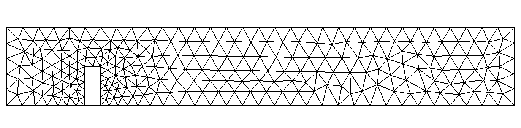
\includegraphics[width=0.7\textwidth]{orig.png}}
  \centerline{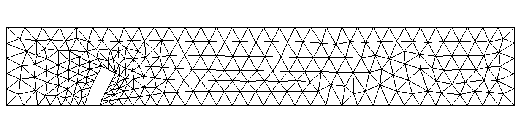
\includegraphics[width=0.7\textwidth]{deform.png}}
  \caption{The original computational mesh (up), and the mesh of the converged solution (down) of a FSI
    computation.}
\end{figure}

%\bibliography{elmerbib}
%\bibliographystyle{plain}


\graphicspath{{./}{helmholtzsolve/}}
\chapter{Helmholtz Solver}

\modinfo{Module name}{HelmholtzSolve}
\modinfo{Module subroutines}{\Idx{HelmholtzSolver}}
\modinfo{Module authors}{Juha Ruokolainen, Mikko Lyly}
\modinfo{Document authors}{Juha Ruokolainen}
\modinfo{Document edited}{March 30th 2006}

\section{Introduction}

This module solves the Helmholtz equation, which is the Fourier transform
of the wave equation. 

\section{Theory}

For example, sound propagation in air is fairly well described by the
wave equation:
\begin{equation}
\frac{1}{c^2}\frac{\partial^2 p}{\partial t^2} - \nabla^2p  = 0.
\end{equation}

When linear the equation may be written in frequency space as
\begin{equation}
k^2 P + \nabla^2P  = 0,
\end{equation}
where $k=\omega/c$.
This is the Helmholtz equation.
The instantaneous pressure may be computed
from the given field $P$:
\begin{equation}
p(t) = \Re(P e^{i\omega t}) = \Re(P)\cos(\omega t) - \Im(P)\sin(\omega t),
\end{equation}
where $i=\sqrt{-1}$ is the imaginary unity.

In Elmer  the equation has an added term which is proportional
to first time derivative of the field, whereupon the equation becomes
\begin{equation}
(k^2 - ikD)P + \nabla^2P  = 0,
\label{eq-sdamp}
\end{equation}
where $D$ is the damping factor.


\subsection{Boundary Conditions}

The usual boundary condition for the Helmholtz equation is to
give the flux on the boundary:
\begin{equation}
\nabla P\cdot\Vec{n} = g,
\end{equation}
also Dirichlet boundary conditions may be set.
The Sommerfeldt or far field boundary condition is as follows
\begin{equation}\label{Sommerfeldt-bc}
\nabla P\cdot\Vec{n} + \frac{i\omega}{Z}P = 0,
\end{equation}
where the complex-valued quantity $Z$ may be defined by the user.
It is noted that incoming and outgoing waves may be approximated by
setting $Z=\pm c$, respectively.
%the plus and minus describe incoming and outgoing waves respectively.


\section{Keywords} 

\sifbegin

\sifitem{Simulation}{}
This section gives values to parameters concerning the simulation
as whole.
\sifbegin
\sifitem{Frequency}{Real}
Give simulation frequency in units of $1/\mathrm{s}$.
Alternatively use the {\tt Angular Frequency} keyword.
\sifitem{Angular Frequency}{Real}
Give simulation frequency in units of $1/\mathrm{rad}$.
Alternatively use the {\tt Frequency} keyword.
\sifend

\sifitem{Solver}{solver id} 
Note that all the keywords related to linear solver (starting
with {\tt Linear System})
may be used in this solver as well.  They are defined elsewhere. 
Note also that for the Helmholtz equation {\tt ILUT} preconditioning
works well.

\sifbegin
\sifitem{Equation}{String [Helmholtz]} 
The name of the equation.
\sifitem{Procedure}{File ["HelmholtzSolve"\ "HelmholtzSolver"]}
This keyword is used to give the Elmer solver the place where
to search for the Helmholtz equation solver.
\sifitem{Variable}{String [Pressure]}
Give a name to the field variable.
\sifitem{Variable DOFs}{Integer [2]}
This keyword must be present, and {\it must} be set to the value $2$.
\sifitem{Bubbles}{Logical}
If set to {\tt True} this keyword activates the bubble stabilization.
\sifend

\sifitem{Equation}{eq id}
The equation section is used to define a set of equations for a body or set of bodies:
\sifbegin
\sifitem{Helmholtz}{Logical} If set to {\tt True}, solve the Helmholtz equation,
the name of the variable must match the {\tt Equation} setting in the {\tt Solver} section.
\sifend


\sifitem{Initial Condition}{ic id} 
The initial condition section may be used to set initial values for the field
variables. The following variables are active:
\sifbegin
\sifitem{Pressure i}{Real} 
For each the real and imaginary parts of the solved field {\tt i}$=1,2$.
\sifend

\sifitem{Material}{mat id}
The material section is used to give the material parameter values. The
following material parameters may be set in Helmholtz equation.
\sifbegin
\sifitem{Sound Speed}{Real} 
This keyword is use to give the value of the speed of sound.
\sifitem{Sound Damping}{Real} 
This keyword is use to give the value of the damping factor $D$ in
equation \ref{eq-sdamp}.
\sifend


\sifitem{Boundary Condition}{bc id}
The boundary condition section holds the parameter values for various
boundary condition types. Dirichlet boundary conditions may be
set for all the primary field variables. The one related to Helmholtz equations
are
\sifbegin
\sifitem{Pressure i}{Real} 
Dirichlet boundary condition
for real and imaginary parts of the variable.
Here the values {\tt i}$=1,2$ correspond to the real and 
imaginary parts of the unknown field.
\sifitem{Wave Flux 1,2}{Real}
Real and imaginary parts of the boundary flux.
Here the values {\tt i}$=1,2$ correspond to the real and 
imaginary parts of the boundary flux.
\sifitem{Wave Impedance 1,2}{Real}
This keyword may be used to define the real and imaginary parts of
the quantity $Z$ in (\ref{Sommerfeldt-bc}).
Here the values {\tt i}$=1,2$ correspond to the real and 
imaginary parts of $Z$.
%Real and imaginary parts of the boundary impedance {\tt i}$=1,2$.
%The impedance is used to compute the boundary wave number for the
%Sommerfeldt boundary condition:
%\begin{equation}
%k = \frac{\omega}{\mathrm{impedance}}.
%\end{equation}
\sifend
\sifend


%\bibliography{elmerbib}
%\bibliographystyle{plain}


\graphicspath{{./}{poissonbem/}}
\Chapter{BEM Solver for Poisson Equation}

\modinfo{Module name}{PoissonBEM}
\modinfo{Module subroutines}{\Idx{PoissonBEMSolver}}
\begin{versiona}
\modinfo{Module authors}{Juha Ruokolainen}
\modinfo{Document authors}{Juha Ruokolainen}
\modinfo{Document edited}{May 27th 2003}

\section{Introduction}

This module solves the Laplace equation by \Idx{boundary element method} (\Idx{BEM}), where
the differential equation is transformed to integral equation along the
boundaries. On the boundaries either potential or normal flux may be defined.
A source term may be included (Poisson equation), but the source term remains
a volume integral.

\section{Theory}

The Poisson equation is mathematically described as
\begin{equation}
-\Delta \Phi - f = 0, \mbox{ in } \Omega,
\end{equation}
where $f$ is the given source.

In BEM we transform this equation to \Idx{integral equation} over boundaries. We start
by multiplying the equation by a weight function and integrating over the volume,
and integrating by parts
\begin{equation}
-\int_\Omega \Delta \Phi w\ d\Omega  = \int_\Omega \nabla\Phi\cdot \nabla w\ d\Omega  -
\int_\Gamma \frac{\partial\Phi}{\partial n} w\ d\Gamma.
\end{equation}
Similarily we may write an equation reversing the roles of $\Phi$ and $w$
\begin{equation}
-\int_\Omega \Delta w \Phi\ d\Omega = \int_\Omega \nabla w\cdot \nabla \Phi\ d\Omega  -
\int_\Gamma \frac{\partial w}{\partial n} \Phi\ d\Gamma.
\end{equation}
Substracting the two equations we have
\begin{equation}
-\int_\Omega \Delta \Phi w\ d\Omega =
-\int_\Omega \Delta w \Phi\ d\Omega -
\int_\Gamma \frac{\partial\Phi}{\partial n} w\ d\Gamma +
\int_\Gamma \frac{\partial w}{\partial n} \Phi\ d\Gamma
\end{equation}
Next we choose the weight $w$ as follows:
\begin{equation}
-\Delta w = \delta_r(r'),
\end{equation}
so that 
\begin{equation}
-\int_\Omega \Delta w \Phi\ d\Omega = \Phi(r), 
\end{equation}
The weight $w$ chosen this way is the Green's function for the Laplace operator,
i.e.

\begin{equation}
 w(r,r') = \frac{\log(r-r')}{2\pi} \mbox{ in 2d }, 
 w(r,r') = \frac{1}{4\pi(r-r')} \mbox{ in 3d }.
\end{equation}

Finally we add the source term, and we have the equation
\begin{equation}
\Phi(r) -
\int_\Gamma \frac{\partial\Phi}{\partial n} w\ d\Gamma +
\int_\Gamma \frac{\partial w}{\partial n} \Phi\ d\Gamma - \int_\Omega fw\ d\Omega = 0.
\end{equation}
Only the source term is now integrated over the volume.
This equation may now be discretized by standard methods.

\subsection{Boundary Conditions}

Boundary conditions may be set for either potential
\begin{equation}
\Phi = \Phi_\Gamma \mbox{ on } \Gamma,
\end{equation}
or normal flux
\begin{equation}
-\frac{\partial \Phi}{\partial n} = g \mbox{ on } \Gamma.
\end{equation}



\section{Keywords} 
\end{versiona}

\sifbegin

\sifitem{Solver}{solver id} 
Note that all the keywords related to linear solver (starting with {\tt Linear System})
may be used in this solver as well.
They are defined elsewhere.  Note also that the BEM discretization
results to a full linear system in contrast to FEM discretizations
and the ILU preconditioning settings are not available.

\sifbegin
\sifitem{Equation}{String [PoissonBEM]} 
The name of the equation.
\sifitem{Procedure}{File ["PoissonBEM"\ "PoissonBEMSolver"]}
This keyword is used to give the Elmer solver the place where
to search for the  equation solver.
\sifitem{Variable}{String [Potential]}
Give a name to the field variable.
\sifitem{Variable DOFs}{Integer [1]}
This keyword must be present, and {\it must} be set to the value $1$.
\sifitem{Exported Variable 1}{String Flux}
If this keyword is given, the output will include the normal flux at
boundaries, the name must be exactly as given.
\sifitem{Exported Variable 1 DOFs}{Integer [1]}
This keyword must be present if Flux values are to be computed,
and {\it must} be set to the value $1$.
\sifend

\sifitem{Equation}{eq id}
The equation section is used to define a set of equations for a body or set of bodies:
\sifbegin
\sifitem{PoissonBEM}{Logical} if set to {\tt True}, solve the Poisson equation,
the name of this parameter must match the {\tt Equation} setting in the {\tt Solver} section.
\sifend
If the mesh has any volume elements with a body id that corresponds to a body where to
the Poisson equation is activated, the value of the potential is computed for these elements
as a postprocessing step. Note that the computation of potential is not a trivial task,
so large number of volume elements may result to long execution time.

\sifitem{Boundary Condition}{bc id}
The boundary condition section holds the parameter values for various
boundary condition types. Dirichlet boundary conditions may be
set for all the primary field variables. The one related to Poisson (BEM) equation
are
\sifbegin
\sifitem{Body Id}{Integer}
Give body identification number for this boundary, used to reference
body definitions in .sif file. This parameter must be set so that the ElmerSolver
knows at which boundaries to solve the corresponding equation.
\sifitem{Potential}{Real} 
Known potential value at boundary.
\sifitem{Flux}{Real}
Known normal flux at boundary.
\sifitem{Normal Target Body}{Integer}
The direction of boundary normals are important for the success of the computation. They
should point consistently outward from the boundaries. This is accomplished either if
the mesh generator automatically orients the boundary elements consistently, or including
in the mesh the parent (volume) elements of the boundaries and using this keyword. The value
-1 of this parameter points to the side where there are no volume elements. If the parameter
gets the value of the body id of the volume elements, the normal will point to that direction.
\sifend

\sifitem{Body Force}{bf id}
The source term for the Poisson equation may be given here. The volume integral
is computed on a body with a volume mesh and the PoissonBEM equation set to true.
\sifbegin
\sifitem{Source}{Real}
The source term for the Poisson equation.
\sifend
\sifend


%\bibliography{elmerbib}
%\bibliographystyle{plain}



\graphicspath{{./}{helmholtzbem/}}
\chapter{BEM Solver for Helmholtz Equation}

\modinfo{Module name}{HelmholtzBEM}
\modinfo{Module subroutines}{\Idx{HelmholtzBEMSolver}}
\begin{versiona}
\modinfo{Module authors}{Juha Ruokolainen}
\modinfo{Document authors}{Juha Ruokolainen}
\modinfo{Document edited}{May 27th 2003}

\section{Introduction}

This module solves the Helmholtz equation by \Idx{boundary element method} (\Idx{BEM}), where
the differential equation is transformed to \Idx{integral equation} along the
boundaries. On the boundaries either pressure or normal flux may be defined.

\section{Theory}

The Helmholtz equation is mathematically described as
\begin{equation}
(k^2+\Delta ) \Phi  = 0, \mbox{ in } \Omega.
\end{equation}

In BEM we transform this equation to integral equation over boundaries. We start
by multiplying the equation by a weight function and integrating over the volume,
and integrating by parts
\begin{equation}
\int_\Omega (k^2+\Delta \Phi) w\ d\Omega  =
\int_\Omega k^2 w\Phi d\Omega -
\int_\Omega \nabla\Phi\cdot \nabla w\ d\Omega +
\int_\Gamma \frac{\partial\Phi}{\partial n} w\ d\Gamma.
\end{equation}
Similarily we may write an equation reversing the roles of $\Phi$ and $w$
\begin{equation}
\int_\Omega (k^2+\Delta) w \Phi\ d\Omega =
\int_\Omega k^2 w\Phi d\Omega -
\int_\Omega \nabla w\cdot \nabla \Phi\ d\Omega  +
\int_\Gamma \frac{\partial w}{\partial n} \Phi\ d\Gamma.
\end{equation}
Substracting the two equations we have
\begin{equation}
\int_\Omega (k^2+\Delta) \Phi w\ d\Omega =
\int_\Omega (k^2+\Delta) w \Phi\ d\Omega -
\int_\Gamma \frac{\partial\Phi}{\partial n} w\ d\Gamma +
\int_\Gamma \frac{\partial w}{\partial n} \Phi\ d\Gamma
\end{equation}
Next we choose the weight $w$ as follows:
\begin{equation}
(k^2+\Delta)w = \delta_r(r'),
\end{equation}
so that 
\begin{equation}
\int_\Omega (k^2+\Delta) w \Phi\ d\Omega = \Phi(r), 
\end{equation}
The weight $w$ chosen this way is the \Idx{Green's function} for the Helmholtz operator,
i.e.

\begin{equation}
 w(r,r') = \frac{1}{i4}H_0(k(r-r')) \mbox{ in 2d }, 
 w(r,r') = \frac{1}{4\pi}\exp^{-ik(r-r')} \mbox{ in 3d },
\end{equation}
where $H_0$ is the Hankel function.

Finally we have the equation
\begin{equation}
\Phi(r) -
\int_\Gamma \frac{\partial\Phi}{\partial n} w\ d\Gamma +
\int_\Gamma \frac{\partial w}{\partial n} \Phi\ d\Gamma = 0.
\end{equation}

\subsection{Boundary Conditions}

Boundary conditions may be set for either pressure
\begin{equation}
\Phi = \Phi_\Gamma \mbox{ on } \Gamma,
\end{equation}
or normal flux
\begin{equation}
-\frac{\partial \Phi}{\partial n} = g \mbox{ on } \Gamma.
\end{equation}


\section{Keywords} 
\end{versiona}

\sifbegin

\sifitem{Simulation}{}
\sifbegin
\sifitem{Angular Frequency}{Real}
Give the value of the angular frequency for the simulation.
\sifend

\sifitem{Solver}{solver id} 
Note that all the keywords related to linear solver (starting with {\tt Linear System})
may be used in this solver as well.
They are defined elsewhere.  Note also that the BEM discretization
results to a full linear system in contrast to FEM discretizations
and the ILU preconditioning settings are not available.

\sifbegin
\sifitem{Equation}{String [HelmholtzBEM]} 
The name of the equation.
\sifitem{Procedure}{File ["HelmholtzBEM"\ "HelmholtzBEMSolver"]}
This keyword is used to give the Elmer solver the place where
to search for the  equation solver.
\sifitem{Variable}{String [Pressure]}
Give a name to the field variable.
\sifitem{Variable DOFs}{Integer [2]}
This keyword must be present, and {\it must} be set to the value $2$.
\sifitem{Exported Variable 1}{String Flux}
If this keyword is given, the output will include the normal flux at
boundaries, the name must be exactly as given.
\sifitem{Exported Variable 1 DOFs}{Integer [2]}
This keyword must be present if Flux values are to be computed,
and {\it must} be set to the value $2$.
\sifend

\sifitem{Equation}{eq id}
The equation section is used to define a set of equations for a body or set of bodies:
\sifbegin
\sifitem{HelmholtzBEM}{Logical} if set to {\tt True}, solve the Helmholtz equation,
the name of this parameter must match the {\tt Equation} setting in the {\tt Solver} section.
\sifend
If the mesh has any volume elements with a body id that corresponds to a body where to
the Helmholtz equation is activated, the value of the pressure is computed for these elements
as a postprocessing step. Note that the computation of potential is not a trivial task,
so large number of volume elements may result to long execution time.

\sifitem{Boundary Condition}{bc id}
The boundary condition section holds the parameter values for various
boundary condition types. Dirichlet boundary conditions may be
set for all the primary field variables. The one related to Helmholtz (BEM) equation
are
\sifbegin
\sifitem{Body Id}{Integer}
Give body identification number for this boundary, used to reference
body definitions in .sif file. This parameter must be set so that the ElmerSolver
knows at which boundaries to solve the corresponding equation.
\sifitem{Pressure 1}{Real} 
Known real part of pressure at boundary.
\sifitem{Pressure 2}{Real} 
Known imaginary part of pressure at boundary.
\sifitem{Flux 1}{Real}
Known real part of normal flux at boundary.
\sifitem{Flux 2}{Real}
Known real part of normal flux at boundary.
\sifitem{Normal Taget Body}{Integer}
The direction of boundary normals are important for the success of the computation. They
should point consistently outward from the boundaries. This is accomplished either if
the mesh generator automatically orients the boundary elements consistently, or including
in the mesh the parent (volume) elements of the boundaries and using this keyword. The value
-1 of this parameter points to the side where there are no volume elements. If the parameter
gets the value of the body id of the volume elements, the normal will point to that direction.
\sifend

\sifend


%\bibliography{elmerbib}
%\bibliographystyle{plain}



\graphicspath{{./}{electrostatics/}}
\chapter{Electrostatics}

\modinfo{Directory}{\Idx{Electrostatics}}
\modinfo{Solvers}{\Idx{StatElecSolve}, \Idx{ElectricForce}}
\modinfo{Tools}{\Idx{ElmerGrid}, editor}
\modinfo{Dimensions}{3D, Steady-state}

\subsection*{Case definition}

This case presents solving the Poisson equation for electric potential
and calculating appropriate derived quantities, such as
\Idx{capacitance}, based on the result. The geometry studied is a
symmetric quadrant of a plane capacitor having a rectangular hole in
another plate. A setting of this kind can be used to study the effects
of geometrical features on the capacitance and on the electrostatic
force, which both are meaningful quantities for coupled
simulations in {\em e.g.}  microsystems.


\subsection*{Solution procedure}

The mesh is constructed using ElmerGrid with the following command
\ttbegin
ElmerGrid 1 2 elmesh.grd
\ttend
The mesh is extended above the hole to avoid undesired boundary
effects. The geometry is presented in the Figure~\ref{geo_elstat}

\begin{figure}[hbt]
  \centerline{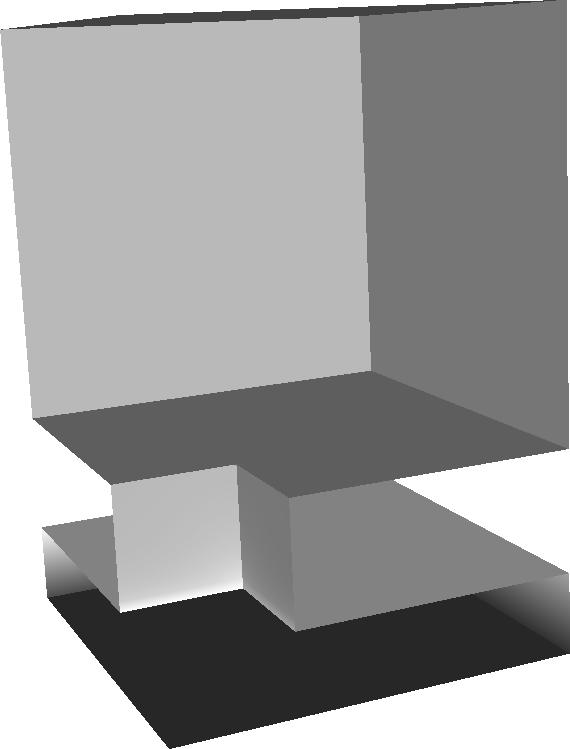
\includegraphics[width=0.32\textwidth]{geo_elstat}}
  \caption{The geometry of problem.} 
  \label{geo_elstat}
\end{figure}

The simulation problem includes a single body, and thus one material
and one equation set, as well as three solvers. The solvers are used
to compute the electric potential and related quantities, to calculate
the electric force, and to save relevant data into a file. This
tutorial is defined in Elmer \Idx{MEMS} units. The sif-file is presented
below.

\ttbegin
Check Keywords Warn

Header
  Mesh DB "." "elmesh"
End
\ttend

Only a single steady state iteration is needed, since the Poisson
equation is linear.
\ttbegin
Simulation
  Coordinate System = Cartesian 3D
  Simulation Type = Steady State
  Steady State Max Iterations = 1
  Output File = "elstatics.result"
  Post File = "elstatics.ep"
End
\ttend

The permittivity of vacuum has to be defined in the Constants section.
\ttbegin
Constants
  Permittivity Of Vacuum = 8.8542e-12
End

Body 1
  Equation = 1
  Material = 1
End
\ttend

Electric energy density is added into the results in Equation
section. This allows energy density to be visualised in
ElmerPost. Note also, that calculating electric flux (or the electric
displacement field) is disabled in the Solver~1 block. Further, the
potential difference used in calculating the capacitance of the system
has to be defined in this section. This should be the same as the
boundary conditions define for the capacitance calculation to be
sensible.
\ttbegin
Equation 1
  Active Solvers(2) = 1 2
  Calculate Electric Energy = True  ! (default False)
End

Solver 1
  Equation = Stat Elec Solver
  Variable = Potential
  Variable DOFs = 1
  Procedure = "StatElecSolve" "StatElecSolver"
  Calculate Electric Field = True  ! (default True)
  Calculate Electric Flux = False  ! (default True)
  Potential Difference = 1.0e6
  Linear System Solver = Iterative
  Linear System Iterative Method = BiCGStab
  Linear System Max Iterations = 200
  Linear System Convergence Tolerance = 1.0e-07
  Linear System Preconditioning = ILU1
  Linear System ILUT Tolerance = 1.0e-03
  Nonlinear System Max Iterations = 1
  Nonlinear System Convergence Tolerance = 1.0e-4
  Nonlinear System Newton After Tolerance = 1.0e-3
  Nonlinear System Newton After Iterations = 10
  Nonlinear System Relaxation Factor = 1
  Steady State Convergence Tolerance = 1.0e-4
End
\ttend

The static electric force solver does not need a lot of
information:
\ttbegin
Solver 2
  Equation = Electric Force
  Procedure = "ElectricForce" "StatElecForce"
End
\ttend

Finally, some data is saved in file scalars.dat in working directory.
\ttbegin
Solver 3
  Exec Solver = After All
  Equation = SaveScalars
  Procedure = "\Idx{SaveData}" "SaveScalars"
  Filename = "scalars.dat"
End
\ttend

Only the relative permittivity of the material has to be defined.
\ttbegin
Material 1
  Relative Permittivity = 1
End
\ttend

The boundary conditions include the values of electric potential
(voltage) and indication on which boundary the electric force should
be calculated. On all the other boundaries a natural boundary
condition is used, basically stating that the electric flux through
these boundaries is zero.
\ttbegin
Boundary Condition 1
  Target Boundaries = 4
  Potential = 0.0
  Calculate Electric Force = True
End

Boundary Condition 2
  Target Boundaries = 3
  Potential = 1.0e6
End
\ttend


\subsection*{Results}

The results obtained for capacitance and electric force are compared
to those of a complete plane capacitor. For a plane capacitor, the
capacitance is
\begin{equation}
C=\varepsilon_r\varepsilon_0\frac{A}{d},
\end{equation}
and the electrostatic force is
\begin{equation}
F_e = \frac{1}{2}\varepsilon_r\varepsilon_0\frac{A}{d^2}\Phi^2,
\end{equation}
where $\varepsilon_r$ is the relative permittivity, $\varepsilon_0$
is the permittivity of vacuum, $A$ is the area of a capacitor plate,
$d$ is the separation of the capacitor plates, and $\Phi$ is the
potential difference between the plates.

The results of the simulation as well as the comparison to the
complete plane capacitor values are shown in Table~\ref{tab_elstatics}
(in Elmer MEMS units). Note that the fringe fields on capacitor edges
are not calculated. This would require much larger mesh extending
outside the capacitor boundaries.

\begin{table}[htb]
\caption{Comparison of numerical results to analytic values}
\label{tab_elstatics}
\begin{center}
\begin{tabular}{lccc} \hline
            & simulation & analytic & ratio \\ \hline
Capacitance & \ \ $2.1361\cdot 10^{-10}$\ \  & 
              \ \ $2.2136\cdot 10^{-10}$\ \  & 0.965 \\
Electric Force & $1.0406\cdot 10^2$ & 
                 $1.1068\cdot 10^2$ & 0.940 \\ \hline
\end{tabular}
\end{center}
\end{table}

Finally, a picture of the results is presented. The
Figure~\ref{res_elstat} shows the isosurfaces of the electric
potential with the color marking the strength of the electric
field. From the picture it is clearly seen that the electric field is
constant between the plates except for the proximity of the hole which
causes weakening of the field magnitude. There are also strong
electric fields at the edges of the hole.


\begin{figure}[hbt]
  \centerline{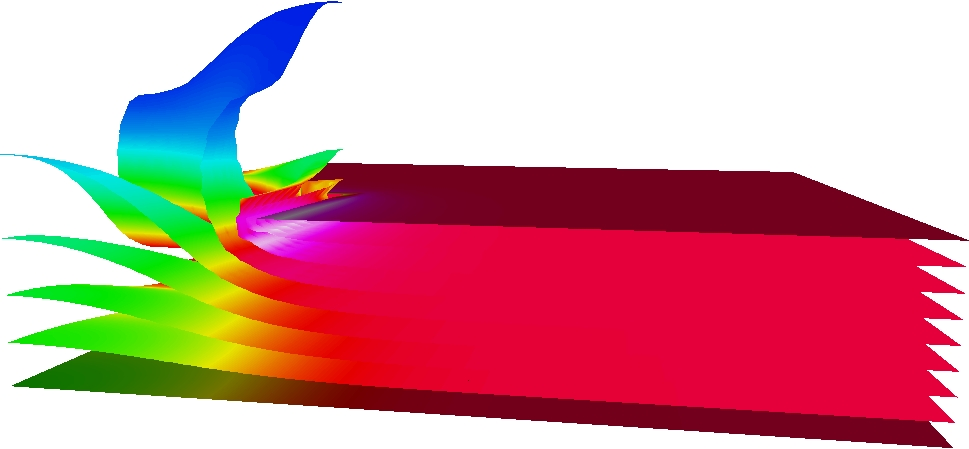
\includegraphics[width=0.8\textwidth]{res_elstat}}
  \caption{Isosurfaces of the potential coloured with electric field
  magnitude.} 
  \label{res_elstat}
\end{figure}



\vfill
\mbox{}



\graphicspath{{./}{statcurrent/}}
\Chapter{Static Current Conduction}\label{chap:statcurr}

\modinfo{Module name}{\Idx{StatCurrentSolve}}
\modinfo{Module subroutines}{\Idx{StatCurrentSolver}}

\begin{versiona}
\modinfo{Module authors}{Leila Puska, Antti Pursula, Peter R�back}
\modinfo{Document authors}{Antti Pursula}
\modinfo{Document edited}{August 2nd 2002}


\section{Introduction}

The macroscopic electromagnetic theory is governed by the Maxwell's
equations. This module solves the electrostatic potential in
conducting medium allowing volume currents and electric power loss
(Joule heating) to be derived.


\section{Theory}

In quasi-static approximation, when $\varepsilon \mu c^2 << 1$, the
first and fourth Maxwell equation can be written as follows
\begin{eqnarray}
\nabla\cdot \Vec{D} & = & \rho \label{max1} \\
%\nabla\cdot \Vec{B} & = & 0 \\
%\nabla\times \Vec{E} & = & -\frac{\partial\Vec{B}}{\partial t} \\
\nabla\times \Vec{H} & = & \Vec{J} + \frac{\partial\Vec{D}}{\partial t}
\label{max4}
\end{eqnarray}

The continuity equation for electric charges is
easily derived from the above Maxwell Eqs.~\ref{max1} and~\ref{max4}
\begin{equation}
\frac{\partial \rho}{\partial t} + \nabla\cdot \Vec{J} = 0
\label{elcontinuity}
\end{equation}
The \Idx{Ohm's law} for conducting material gives
the relationship between \Idx{current density} and 
electric field,
\begin{equation}
\Vec{J} = \sigma \Vec{E}
\label{ohm}
\end{equation}
In steady-state case the electric field may be expressed with a help of
an electric scalar potential $\phi$, 
\begin{equation}
\Vec{E} = -\nabla \phi . 
\label{elpot}
\end{equation}

Starting from the continuity equation~\ref{elcontinuity} and using
Eqs.~\ref{ohm} and~\ref{elpot} we get
\begin{equation}
\nabla\cdot\sigma\nabla\phi = \frac{\partial\rho}{\partial t}.
\end{equation}
This Poisson equation is used to solve the electric potential. The
source term is often zero but in some cases it might be necessary.

The volume current density is now calculated by
\begin{equation}
\vec{J} = -\sigma\nabla\phi,
\end{equation}
and electric power loss density which is turned into heat by
\begin{equation}
h = \nabla\phi\cdot\sigma\nabla\phi.
\end{equation}
The latter is often called the \Idx{Joule heating}. The total heating power
is found by integrating the above equation over the conducting
volume.

\subsection{Boundary Conditions}

For electric potential either Dirichlet or Neumann boundary condition
can be used. The Dirichlet boundary condition gives the value of the
potential on specified boundaries. The Neumann boundary condition is
used to give a current $J_b$ on specified boundaries
\begin{equation}
J_b = \sigma\nabla\phi\cdot\vec{n}.
\end{equation}


\subsection{Power and current control}

Sometimes the desired power or corrent of the system is known a priori.
The control may be applied to the system.
When the electric potential has been computed the heating power may be estimated from
\begin{equation}
 P = \int_\Omega \nabla \phi \cdot \sigma\nabla\phi \, d\Omega .
\end{equation}
If there is a potential difference $U$ in the system the effective resistance may also be
computed from $R=U^2/P$ and the effective current from $I=P/U$. 

The control is achieved by multiplying the potential and all derived field by a suitable variable.
For power control the coefficient is 
\begin{equation}
  C_P = \sqrt{ P_0 / P },
\end{equation}
where $P_0$ is the desired power. For current control the coefficient is 
\begin{equation}
  C_I = I_0 / I,
\end{equation}
where $I_0$ is the desired total current.




\section{Note on output control}

The user can control which derived quantities ({\em i.e.} volume
current and Joule heating) are calculated and additionally specify if
he/she wants to output also the electric conductivity. The latter is
useful when the conductivity depends for example on temperature. This
feature is available only for isotropic (scalar) conductivities.

There are also available two choises of visualization types for the
derived quantities. The node values can be calculated by taking the
average of the derived values on neighbouring elements (constant
weights). This results often in visually good images. The other
possible choice is to weight the average with the size of the
elements, which is more accurate and should be used when some other
variable depends on these derived values. The latter choice is also
the default.


\section{Keywords}
\end{versiona}

\sifbegin
\sifitemnt{Solver}{solver id}
\sifbegin
\sifitemnt{Equation}{String Stat Current Solver}
\sifitem{Variable}{String Potential}
This may be of any name as far as it is used consistently also elsewhere.
\sifitem{Variable DOFs}{Integer 1}
Degrees of freedom for the potential.
\sifitem{Procedure}{File "StatCurrentSolve"\ "StatCurrentSolver"}
Following are listed three keywords with default values
for output control.
\sifitemnt{Calculate Volume Current}{Logical [True]}
\sifitemnt{Calculate Joule Heating}{Logical [True]}
\sifitem{Constant Weights}{Logical [True]}
Used to turn constant weighting on for the results.
\sifitem{Power Control}{Real} 
Apply power control with the desired heating power being $P_0$.
\sifitem{Current Control}{Real} 
Apply current control with the desired current being $I_0$.
\sifend

\sifitemnt{Material}{mat id}
\sifbegin
\sifitemnt{Electric Conductivity}{Real}
\sifend

\sifitemnt{Body Force}{bodyforce id}
\sifbegin
\sifitem{Current Source}{Real}
Possibility for a current source, not used often though.
\sifitem{Joule Heat}{Logical}
If this flag is active the Heat equation will automatically compute the 
quantity $\nabla \phi \cdot \sigma\nabla\phi$ as heat source.
Then it is assumed that $\phi$ is named \texttt{Potential}.
If there is no heat equation this flag has no effect.
\sifend

\sifitemnt{Boundary Condition}{bc id}
\sifbegin
\sifitem{Potential}{Real}
Dirichlet BC for the potential.
\sifitem{Current Density BC}{Logical}
Must be set to {\tt True} if Neumann BC is used.
\sifitem{Current Density}{Real}
Neumann boundary condition for the current.
\sifend
\sifend

\begin{versiona}
\bibliography{elmerbib}
\bibliographystyle{plain}
\end{versiona}



\graphicspath{{./}{magnetostatics/}}
\Chapter{Magnetostatics}
\noindent
\modinfo{Module name}{StatMagSolve}
\modinfo{Module subroutines}{\Idx{StatMagSolver}}
\begin{versiona}
\modinfo{Module authors}{Juha Ruokolainen, Ville Savolainen, Jussi Heikonen, Peter R�back, Antti Pursula}
\modinfo{Document authors}{Ville Savolainen, Peter R�back, Antti Pursula}
\modinfo{Document edited}{June 29th 2006}

\section{Introduction}

The Maxwell's equations may generally be expressed with 
a scalar and a vector potential. The magnetic field is then
the curl of the vector potential. In some cases the scalar potential vanishes
and the system is fully described by the vector potential. These
cases includes magnetostatics and time-harmonic induction at low frequencies.

Magnetostatics\index{magnetostatics} describes the time-independent magnetic
fields. The magnetic field may be created by electromagnets with given current
distributions or permanent ferromagnets. This solver allows the first option,
with non-homogeneous and non-linear magnetic materials. 

In some cases the current density varies sinusoidally with time.
If the field varies slowly and there are no conductors in the system
the problem is described with the stationary model. However, in conductors the
magnetic field results in additional currents that make the equation
complex.

%%Currently only an axisymmetric version of the solver is provided.



\section{Theory}

When there are no hard ferromagnets, the magnetostatics problems may be
expressed with magnetic vector potential $\vec{A}$ that satisfies
$\vec{B} = \nabla\times\vec{A}$. It is obtained directly
from the Amp\`{e}re's law, with displacement current ignored, that
\[
\nabla \times \left(\frac{1}{\mu} \nabla \times \vec{A} \right) = \vec{\jmath}.
\]
Here $\mu$ is the magnetic permeability of the material. The equation may be
non-linear through the magnetic permeability curve of a ferromagnetic material.
The magnetic permeability is specified in the {\tt Material} section by the
keyword {\tt Magnetic Permeability}.

The equation above may be solved either in axial symmetry or in three
dimensions. In 3D, a curl vector identity is used to transform the
equation into the form
\[
-\frac{1}{\mu} \nabla^2\vec{A} = \vec{\jmath},
\]
which is valid when $\mu$ is not a function of space
coordinates. Also, the vector potential $\vec{A}$ is {\em a priori}
assumed to satisfy the Coulomb gauge ($\nabla\cdot\vec{A}=0$).


If there are conductors in the system the electric field is obtained
from 
\[
  \vec{E} = \sigma \Der{\vec{A}}{t},
\]
where $\sigma$ is the electrical conductivity. In time-harmonic case 
the current density is sinusoidal
  $\vec{\jmath} = \vec{\jmath}_0 e^{i \omega t}$,
where $\omega=2\pi f$ is the angular frequency.
Using a trial $\vec{A}=\vec{A}_0 e^{i \omega t}$ we obtain an equation
for the amplitude
\[
\nabla \times \left(\frac{1}{\mu} \nabla \times \vec{A}_0 \right) 
+ i \omega \sigma \vec{A}_0 = \vec{\jmath}_0.
\]

If the geometry is axisymmetric, then the magnetic flux density $\vec{B}$ has
only $r$- and $z$-components, and the current density $\vec{\jmath}$ and the
vector potential $\vec{A}$ only $\phi$-components, and
\begin{equation}
\nabla \times \left(\frac{1}{\mu} \nabla \times A_{\phi}\vec{e}_{\phi}\right)
+ i \omega \sigma A_{\phi}\vec{e}_{\phi} =j_{\phi}\vec{e}_{\phi}.\label{magnetostatic}
\end{equation}
The current density is given as a body force with the keyword {\tt Current
Density}. The vector potential satisfies now automatically the Coulomb gauge.

In stady state case $A_\phi$ is real and there is only one unknown.
In the harmonic case the equation has two unknowns 
-- the in-phase and the out-of-phase component of
the vector potential. After solution the heat generation in the conductors
may be computed from 
\[
  h = \frac{1}{2} \sigma \omega^2 | \vec{A}_0 |^2 .
\]

The magnetic flux density is calculated as a post-processing step from the
vector potential. Both the vector potential and the magnetic flux density
components are written in the result and ElmerPost files. The variable names
in the result file are {\tt magnetic vector potential} and {\tt magnetic flux
density 1}, {\tt 2} and {\tt 3}.

By definition, magnetostatics deals with steady-state problems. However, the
problem may be solved nominally time-dependent. This merely means that it is
solved for a set of given current densities.

\subsection{Boundary Conditions}

For the magnetostatics equation one can apply either Dirichlet or natural
boundary conditions. In both cases, one must check that the computational
domain is extended far enough to avoid numerical errors.

The \Idx{Dirichlet boundary condition} for $A_\phi$ is
\begin{equation}
A_\phi = A_\phi^b.
\end{equation}
In practice, when Dirichlet condition is used, usually $A_\phi^b=0$.
The keyword for the Dirichlet boundary condition is
{\tt Magnetic Vector Potential}. If Dirichlet condition is not specified,
natural boundary condition is used.

\section{Keywords} 
\end{versiona}

\sifbegin
\sifitem{Solver}{solver id} 
Note that all the keywords related to linear solver (starting with {\tt Linear System}) 
may be used in this solver as well.
They are defined elsewhere. 

\sifbegin
\sifitem{Equation}{String [Static Magnetic Field]} 
The name of the equation.
\sifitem{Variable}{String [Magnetic Vector Potential]}
The name of the variable.
\sifitem{Procedure}{File ["StatMagSolve"\ "StatMagSolver"]}
The name of the file and subroutine.
\sifitem{Calculate Magnetic Flux}{Logical [True]}
In large computations the automatic computation of the magnetic flux may be turned off
by this keyword. The default is \texttt{True}.
\sifitem{Calculate Joule Heating}{Logical [True]}
In large computations the automatic computation of the Joule heating may be turned off
by this keyword. The default is \texttt{True}. The keyword is only applicable 
for the harmonic case. The computation results to two additional 
variables. \texttt{Joule Heating} gives the absolute heating and 
\texttt{Joule Field} the field that gives the heating when multiplied
by the electric conductivity. This may be needed if the electric conductivity is 
discontinuous making also the heating power discontinuous. 
\sifitem{Desired Heating Power}{Real}
A constant that gives the desired total heating power in Watts. If the keyword is active
the the \texttt{Joule Heating} and \texttt{Joule Field} are multiplied by the ratio of
the desired and computed heating powers.
\sifitem{Nonlinear System Convergence Tolerance}{Real} This keyword gives a criterion to
terminate the nonlinear iteration after the relative change of the norm of the field variable
between two consecutive iterations $k$ is small enough
$$
 ||A_\phi^k-A_\phi^{k-1}|| < \epsilon ||A_\phi^k||,
$$
where $\epsilon$ is the value given with this keyword.
\sifitem{Nonlinear System Max Iterations}{Integer} 
The maximum number of nonlinear iterations the
solver is allowed to do. If neither the material parameters nor the boundary
conditions are functions of the solution the problem is linear,
this should be set to 1.
\sifitem{Nonlinear System Relaxation Factor}{Real} Giving this keyword triggers the use
of  relaxation in the nonlinear equation solver.
Using a factor below unity is sometimes required to achive convergence of the nonlinear system.
A factor above unity might speed up the convergence. Relaxed variable is defined as follows:
$$
 A_\phi^{'} = \lambda A_\phi^k + (1-\lambda) A_\phi^{k-1},
$$
where $\lambda$ is the factor given with this keyword. The default value for the relaxation factor
is unity.
\sifend

\sifitem{Equation}{eq id}
The equation section is used to define a set of equations for a body or set of bodies:
\sifbegin
\sifitem{Static Magnetic Field}{Logical} If set to {\tt True}, solve the
magnetostatics equation.
\sifitem{User Defined Velocity}{Logical} If set to {\tt True} uses a
given velocity instead of the computed velocity. The values of the
velocity may be given in the {\tt Material} section.
\sifend

\sifitem{Body Force}{bf id}
The body force section may be used to give additional force terms for the equations.
\sifbegin
\sifitem{Current Density}{Real} Specifies the azimuthal component of the
current density. May be a positive or negative constant or a function of a
given variable.
\sifitem{Current Phase Angle}{Real} Specifies the phase angle of the current
density in degrees. The default phase angle is zero. Applies only to the 
time-harmonic case.
\sifend

\sifitem{Initial Condition}{ic id} 
The initial condition section may be used to set initial values for the field
variables. The following variable is active:
\sifbegin
\sifitem{Magnetic Vector Potential}{Real} 
The azimuthal component of the magnetic vector potential.
\sifend

\sifitem{Material}{mat id}
The material section is used to give the material parameter values. 
Material parameter available for the magnetostatics equation are.
\sifbegin
\sifitem{Magnetic Permeability}{Real} The magnetic permeability $\mu$ is set
with this keyword, defining the material relation $\vec{B}=\mu\vec{H}$.
The magnetic permeability may be a constant (default is $4\pi 10^{-7}$) 
or a function of a given variable,
typically given by the relation $\mu=\mu(|\vec{B}|)$. The value of the
magnetic flux density $|\vec{B}|$ is available by the variable named.
{\tt Absolute Magnetic Flux}.
\sifitem{Electrical Conductivity}{Real} 
The electrical conductivity defines the relation $\vec{\jmath}=\sigma \vec{E}$.
Only isotropic case is possible.
The parameter is needed only in the time-harmonic case.
\sifitemnt{MHD Velocity 1}{Real}
\sifitemnt{MHD Velocity 2}{Real}
\sifitem{MHD Velocity 3}{Real}
The components of the user defined velocity.
\sifend

\sifitem{Boundary Condition}{bc id}
The boundary condition section holds the parameter values for various
boundary condition types. Dirichlet boundary condition may be
set for the vector potential. The one related to the the axisymmetric
magnetostatics problem is
\sifbegin
\sifitem{Magnetic Vector Potential}{Real} 
The azimuthal component of the magnetic vector potential.
\sifend

\sifend



%\bibliography{elmerbib}
%\bibliographystyle{plain}


\graphicspath{{./}{mhd/}}
\chapter{Induction Equation}
\noindent
\modinfo{Module name}{included in solver / MagneticSolve as external procedure}
\modinfo{Module subroutines}{\Idx{MagneticSolver}}
\begin{versiona}
\modinfo{Module authors}{Juha Ruokolainen}
\modinfo{Document authors}{Ville Savolainen, Antti Pursula}
\modinfo{Document edited}{May 24th 2005}

\section{Introduction}

The magnetic \Idx{induction equation} describes interaction of a conducting
liquid or gas with applied and induced magnetic fields in the low-frequency
domain. The induction equation for the magnetic flux density is always coupled
to the Navier-Stokes equation for the movement of the fluid. The magnetic
field, in turn, causes the Lorentz force in the Navier-Stokes equation. The
fluid is typically hot, and the Navier-Stokes equation is often coupled also
to the heat equation.

The induction equation solver can also be used in a body without a moving
fluid, i.e., when $\vec{v}=0$ and the Navier-Stokes equation is not solved.
In this case, the problem belongs to the field of magneto-quasistatics.

\section{Theory}

The magnetic induction equation may be derived from the Maxwell's equations,
with the displacement current in Amp\`{e}re's law neglected, and the Ohm's law
for conducting fluids,
$\vec{\jmath} = \sigma ( \vec{E} + \vec{v}\times\vec{B} )$. This approximation
for the behavior of electromagnetic
fields in conducting, moving fluids is called \Idx{magnetohydrodynamics}.

The magnetic induction equation is given by
\begin{equation}
\frac{\partial \vec{B}}{\partial t} + \frac{1}{\sigma\mu}\nabla\times\nabla\times \vec{B} - 
\nabla\times(\vec{v}\times \vec{B}) = 0,\label{induction}
\end{equation}
where $\sigma$ is the electrical conductivity and
$\mu$ the magnetic permeability of the material. These must be specified in the
{\tt Material} section by the
keywords {\tt Electrical Conductivity} and {\tt Magnetic Permeability}.

The force term induced by the magnetic field for the flow momentum equations
is given by
\begin{equation}
\vec{f}_m = \vec{\jmath}\times\vec{B},
\end{equation}
and the Joule heating in the heat equation by
\begin{equation}
h_m = \frac{1}{\sigma}\left|\vec{\jmath}\right|^2,
\end{equation}
where $\vec{\jmath}$ is the current density, calculated from the Amp\`{e}re's
law $\vec{\jmath}=\nabla\times\vec{H}$. These body forces are specified by
the keywords {\tt Lorentz Force} and {\tt Joule Heat}.

The magnetic field can also be divided into external, or applied, and induced
field, $\vec{B}=\vec{B}^e+\vec{B}^i$. The external magnetic field $\vec{B}^e$
is created by permanent magnets or currents outside the fluid. The external
field may be given to the induction equation solver either from a restart file,
e.g., as calculated by the magnetostatic solver, or defined via the sif file's
keywords {\tt Applied Magnetic Field 1}, {\tt 2} and {\tt 3}. If the
restart file is used, the components of $\vec{B}^e$ are read from the variables
named {\tt magnetic flux density 1}, {\tt 2} and {\tt 3}. If both methods are
used, the two applied fields are summed together. It is assumed that the
sources of the external field are outside the flow region, i.e.,
$\nabla\times\vec{B}^e=0$, and that the time derivative of the external field
can be ignored. The time derivative $\partial\vec{B}^e/\partial t$ can,
however, be specified directly by the keywords {\tt Magnetic Bodyforce 1},
{\tt 2} and {\tt 3}. The induction
equation solver gives the components of the induced magnetic field $\vec{B}^i$.

Both transient and steady-state solvers for the magnetohydrodynamical
system (induction, Navier-Stokes and heat equations) are available. The
magnetostatic and time-harmonic solvers for the external magnetic field are
described elsewhere in the Models Manual. In some cases it is also
possible that the velocity is {\em a priori} known, for example when
studying induction in a rotating body. Then a user defined velocity
can be used instead of computing the velocity from Navier-Stokes
equations.

Currently the induction equation can be solved in a cylindrically symmetric or
a general three-dimensional formulation.

\subsection{Boundary Conditions}

For the induction equation one can apply either Dirichlet or natural boundary
conditions. In both cases, one must check that the computational domain is
extended far enough to avoid numerical errors. For this reason, it is possible
to solve the magneto-quasistatics problem in an adjacent body.

The \Idx{Dirichlet boundary condition} for a component of the induced
magnetic field $B_i$ (we have dropped now the superscript $i$ that marked
the induced field) is
\begin{equation}
B_i = B_i^b. 
\end{equation}
$B_i^b$ can be a constant or a function of time, position or other 
variables. The keywords for the Dirichlet boundary conditions are
{\tt Magnetic Field 1}, {\tt 2} and {\tt 3}.

In the cylindrically symmetric case, the Dirichlet boundary
condition for the azimuthal component $B_\phi$ is in the same units as for
the other two components, i.e., in T, and not for a contravariant component.
On the symmetry axis one has to set $B_r = 0$ and $B_\phi = 0$, and
$\partial B_z/\partial r = 0$  is applied implicitly.

If no Dirichlet condition is specified, natural boundary condition is applied.

\section{Keywords} 
\end{versiona}

\sifbegin
\sifitem{Solver}{solver id} 
Note that all the keywords related to linear solver (starting with {\tt Linear System}) may be used in this solver as well.
They are defined elsewhere. 

\sifbegin
\sifitem{Equation}{String [Magnetic Induction]} 
The name of the equation. It is also possible to use this solver as
external procedure. Then the name of the equation must not be the
above (use {\em e.g.} {\tt Magnetic Field Solver}). Also the 
following four keywords have to be added with the values give here.
\sifitemnt{Procedure}{File "MagneticSolve"\ "MagneticSolver"}
\sifitemnt{Variable}{String Magnetic Field}
\sifitemnt{Variable DOFs}{Integer 3}
\sifitem{Exported Variable 1}{= -dofs 3 electric current}
The above four keywords are to be given only when using the solver as
an external procedure.
\sifitem{Nonlinear System Convergence Tolerance}{Real} This keyword gives a criterion to
terminate the nonlinear iteration after the relative change of the norm of the field variable
between two consecutive iterations $k$ is small enough
$$
 ||\vec{B}^k-\vec{B}^{k-1}|| < \epsilon ||\vec{B}^k||,
$$
where $\epsilon$ is the value given with this keyword.
\sifitem{Nonlinear System Max Iterations}{Integer} 
The maximum number of nonlinear iterations the
solver is allowed to do. If neither the material parameters nor the boundary
conditions are functions of the solution, the problem is linear, and
this should be set to 1.
\sifitem{Nonlinear System Relaxation Factor}{Real} Giving this keyword triggers the use
of  relaxation in the nonlinear equation solver.
Using a factor below unity is sometimes required to achive convergence of the nonlinear system.
A factor above unity might speed up the convergence. Relaxed variable is defined as follows:
$$
 \vec{B}^{'} = \lambda \vec{B}^k + (1-\lambda) \vec{B}^{k-1},
$$
where $\lambda$ is the factor given with this keyword. The default value for the relaxation factor
is unity.
\sifitem{Steady State Convergence Tolerance}{Real}
With this keyword a equation specific steady state or coupled system
convergence tolerance is given.
All the active equation solvers must meet their own tolerances for their
variable $u$, before the whole system is deemed converged.
The tolerance criterion is:
$$
 ||u_i-u_{i-1}|| < \epsilon ||u_i||,
$$
where $\epsilon$ is the value given with this keyword.
\sifend

\sifitem{Equation}{eq id}
The equation section is used to define a set of equations for a body or set of bodies:
\sifbegin
\sifitem{Magnetic Induction}{Logical} If set to {\tt True}, solve the magnetic induction equation.
\sifitem{User Defined Velocity}{Logical}
Controls whether the velocity is given by the user or computed by
another solver. Default value is {\tt False}, which means that
velocity solution of Navier-Stokes equations is used.
\sifitem{Navier-Stokes}{Logical} If set to {\tt True}, solve also the
Navier-Stokes equations. For magnetohydrodynamics, this is done, except when
the computational region for the magnetic field is extended beyond the fluid.
\sifitem{Heat Equation}{Logical} If set to {\tt True}, solve also the
heat equation.
\sifend

\sifitem{Body Force}{bf id}
The body force section may be used to give additional force terms for the equations.
\sifbegin
\sifitem{Lorentz Force}{Logical} If set true, triggers the magnetic
field force for the flow momentum equations.
\sifitem{Joule Heat}{Logical} If set true, the Joule heating is added in the
heat equation.
\sifitem{Magnetic Bodyforce i}{Real} This keyword can be used to specify
explicitly the time dependence of the external field, i.e., the term
$-\partial\vec{B}^e/\partial t$. This is especially useful for time-harmonic
fields, where the time derivative can be calculated and expressed easily.
\sifend

\sifitem{Initial Condition}{ic id} 
The initial condition section may be used to set initial values for the field
variables. The following variables are active:
\sifbegin
\sifitem{Magnetic Field i}{Real} 
For each magnetic flux density component {\tt i}$=1,2,3$.
\sifend

\sifitem{Material}{mat id}
The material section is used to give the material parameter values. The
following material parameters may be set for the induction equation. They can
be a constant or a function of a given variable.
\sifbegin
\sifitem{Magnetic Permeability}{Real} The magnetic permeability is set with
this keyword. For most fluids, the vacuum value for $\mu_0$ can be used,
and the keyword set to {\tt 1.25664e-6}.
\sifitem{Electrical Conductivity}{Real} The value of the electrical
conductivity is set with the keyword. For example, for polythermal flows the
conductivity could be a function of the temperature.
\sifitem{Applied Magnetic Field i}{Real} This keyword can be used to specify
the external field, or a part of it, and its contribution to the term
$\nabla\times(\vec{v}\times \vec{B}^e)$. The field may be a function of, e.g.,
time or position.
\sifitemnt{MHD Velocity 1}{Real}
\sifitemnt{MHD Velocity 2}{Real}
\sifitem{MHD Velocity 3}{Real}
The user defined velocity can be given with these keywords.
\sifend

\sifitem{Boundary Condition}{bc id}
The boundary condition section holds the parameter values for various
boundary condition types. Dirichlet boundary conditions may be
set for all the primary field variables. The ones related to induction equation
are
\sifbegin
\sifitem{Magnetic Field i}{Real} 
Dirichlet boundary condition
for each magnetic flux density component {\tt i}$=1,2,3$.
\sifend

\sifend


%\bibliography{elmerbib}
%\bibliographystyle{plain}


\graphicspath{{./}{electrokinetics/}}
\chapter{\Idx{Electrokinetics}}
\noindent
\modinfo{Module name}{\Idx{Electrokinetics}}
\modinfo{Module subroutines}{helmholtz\_smoluchowski1, helmholtz\_smoluchowski2,\\ helmholtz\_smoluchowski3, helmholtz\_smoluchowski, getJouleHeat}
\begin{versiona}
\modinfo{Module author}{Thomas Zwinger}
\modinfo{Document author}{Thomas Zwinger}
\modinfo{Document created}{April 13th 2005}

\section{Introduction}

If dealing with electrolytic fluids constrained to small volumes, surface forces caused by electric surface charges in combination with externally applied electrostatic fields are sufficient strong to affect the fluid volume. If these effects are utilized to attenuate the fluid volume, we talk of \textit{Electrokinetics}. The term \textit{Electroosmotic Flow} (EOF) is used in connection with the attenuation of a net charge inside a originally neutral electrolyte caused by separation induced by a surface charge of a wall.

In most applications utilizing EOF, externally applied fields are sufficient small in order to justify neglecting electric heating (Joule heating) inside the fluid volume. Nevertheless, certain applications, such as High Voltage Capillary Electrophoresis (HV-CE), demand the consideration of this effect \cite{KnoMcC1994}.

\section{Theory}
Chemical reactions between the contents of a liquid and the wall material may lead to a net charge of the containment at the wall-liquid interface. If the liquid is an electrolyte (i.e., it contains free ions), ions of opposite charge align along the wall creating the \textit{Stern layer}. Adjacent to the Stern layer, a charge separation - called the \textit{diffuse layer} of the initially neutral electrolyte takes place. Due to the two layer structure the whole are area of charge separation in the vicinity of a wall is called the \textit{Electric Double layer} (EDL). 
\begin{figure}[tbhp]
%\vspace{-11cm}
\centerline{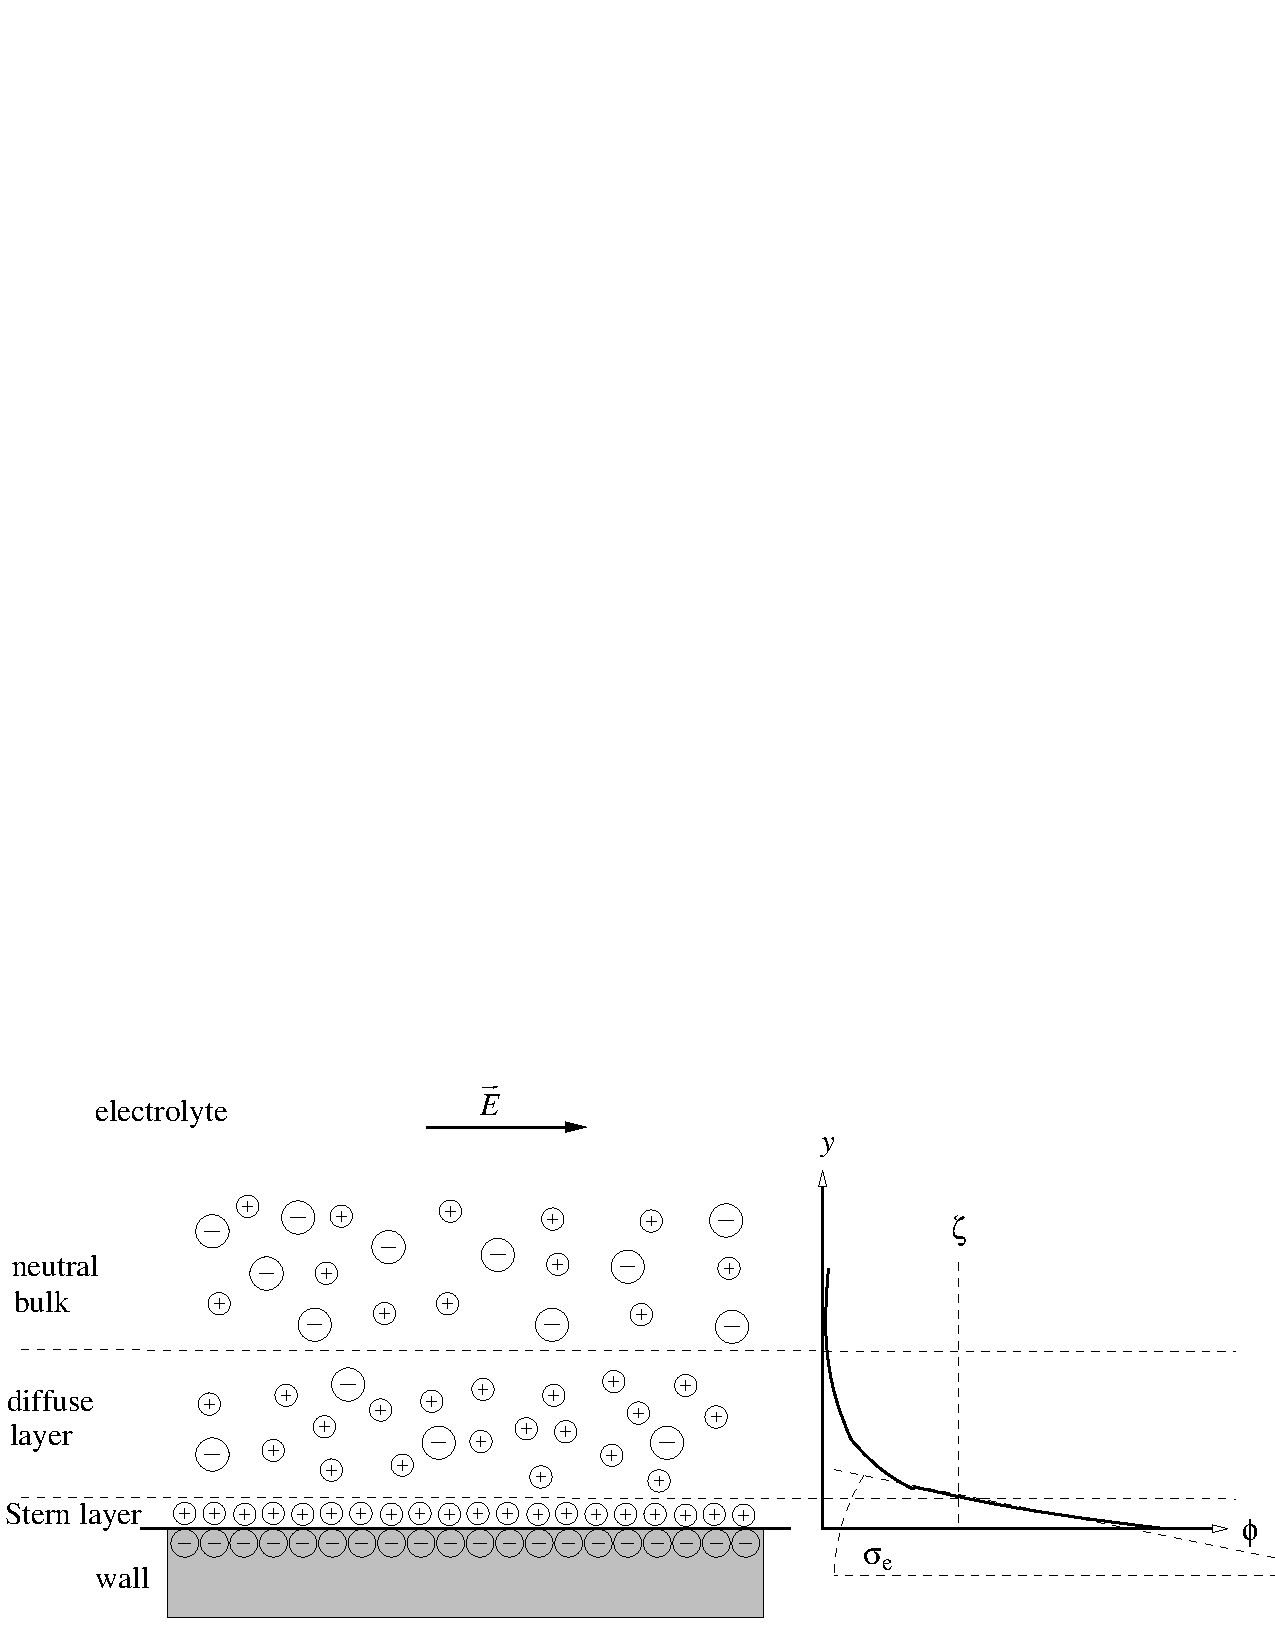
\includegraphics[width=0.9\textwidth]{EDL_bw.pdf}}
\caption{\label{ek:Fig.EDL} Structure of the EDL. The value of the induced potential, $\Phi$ at the Stern layer usually is referred to as the zeta-potential, $\zeta$}
\end{figure}
\subsection{Electroosmotic slip velocity}\label{EOF}
Considering a symmetric electrolyte -- i.e., the bulk ion density of ions with opposite valence numbers $\pm z$ are equal $n^{+}_{0}=n^{-}_{0}=n_{0}$ --  at a certain temperature, $T$, the typical width-scale of the EDL is given by the \textit{Debye length} \cite{KarBes:2001}
\begin{equation}\label{ek:debye}
\lambda_{\mathrm{D}} = \left(\dfrac{\epsilon_{\mathrm{f}}\epsilon_{0}\,k_{\mathrm{b}}\,T_{0}}{2\, n_{0}\, z^{2}\, e^{2}_{0} }\right)^{1/2}.
\end{equation}
Here $e_{0}$ stands for the unit charge and $k_{\mathrm{b}}$ denotes the Boltzmann constant. The relative permittivity of the electrolyte and the permittivity of vacuum are given by $\epsilon_{\mathrm{f}}$ and $\epsilon_{0}$, respectively. 


The potential, $\Phi$ and the volume charge density, $\rho_{e}$, within the EDL are tightly coupled to each other by the Poisson-Boltzmann equation \eqref{eq:poisson-boltzmann} (see chapter \ref{poisson-boltzmann}). In order to exactly resolve the dynamics close to the walls, \eqref{eq:poisson-boltzmann} should be solved and the resulting specific electric force then be considered in the equation of motion. Nevertheless,  provided the typical length scales of the flow perpendicular to the containment walls, $H$, strongly exceed those of the EDL -- in other words, we obtain very small values for the non-dimensional group $\mathcal{L} = \lambda_{\mathrm{D}}/H \ll 1$ -- the dynamics of the electrolyte inside the EDL does not have to be resolved at all. In this case simple considerations of a force balance between shear stress and electric force lead to a slip condition for the fluid \cite{YaFuLi:2001}. At the boundary, the tangential velocity is set to the \textit{Helmholtz-Smoluchowski} velocity
\begin{equation}
\label{ek:helm-smol}
\vec{u}_{\mathrm{tang.}}=\vec{u}_{\mathrm{H-S}} = \frac{\vec{E}_{\mathrm{tang.}}\epsilon_{\mathrm{f}}\epsilon_{0}\zeta}{\mu_{\mathrm{f}}},
\end{equation}
with $\mu_{\mathrm{f}}$ standing for the local fluid viscosity. The \textit{zeta potential}, $\zeta$ -- a property depending on the electric properties of the wall material as well as the electrolyte -- usually is determined experimentally. From a physical point of view it can be interpreted as the value of the solution obtained by \eqref{eq:poisson-boltzmann} at the Stern layer. The tangential component, $\vec{E}_{\mathrm{tang.}}$,  of the external electric field, $\vec{E}$, is evaluated from the outward pointing surface normal $\vec{n}$, applying the following relation
\begin{equation}
\label{ek:etang}
\vec{E}_{\mathrm{tang.}} = \vec{E} - \left(\vec{E}\cdot\vec{n}\right)\vec{n}
\end{equation}
Alternatively, the resulting slip velocity may be related to the tangential field using the \textit{Electroosmotic Mobility}, $\mu_{\mathrm{EOF}}$
\begin{equation}
\label{ek:HS-EOF-mobility}
\vec{u}_{\mathrm{H-S}} = \mu_{\mathrm{EO}}\,\vec{E}_{\mathrm{tang.}}.
\end{equation}
A combination of \eqref{ek:helm-smol} and \eqref{ek:HS-EOF-mobility} leads to the following identity
\begin{equation}
\label{ek:EOF-mobility}
\mu_{\mathrm{EO}} =\frac{\epsilon_{\mathrm{f}}\epsilon_{0}\zeta}{\mu_{\mathrm{f}}}.
\end{equation}

\subsection{Joule Heating}
Due to the small volume in microfluidic applications the additional heat produced by the external electric field needs to be considered. With the local electric conductivity, $\sigma$, and the local volume density, $\rho$, of the electrolyte the specific heat contribution by Joule heating from an external electric field, $\vec{E}$, is given by
\begin{equation}
\label{ek:joule-heating}
h = \sigma\,\vec{E}\cdot\vec{E}/\rho.
\end{equation}
The expression above can be added as body force to the heat transfer equation \eqref{heat_equation}.

\section{Limitations}
\begin{itemize}
\item The Helmholtz-Smoluchowski velocity should not be applied if the non-di\-men\-sion\-al group $\mathcal{L}$ defined in \ref{EOF} is of unity order or larger. Then the potential- and charge density distribution as well as the dynamics of the electrolyte inside the EDL has to be resolved. 
\item In a strict sense, the Helmholtz-Smoluchowski theory applies only to configurations where the normal-component of the external field, $\vec{E}\cdot\vec{n}$, is small. If dealing with electric insulating wall materials -- as it is usually the case in microfluidic applications -- this condition is implicitly complied with. 
\item The assumption of a Newtonian fluid underlies the derivation of the Helmholtz-Smoluchowski velocity.
\item The function \texttt{helmholtz\_smoluchowski} can only be applied on  boundaries of two-dimensional domains, where the tangential direction is uniquely defined.
\item The functions \texttt{helmholtz\_smoluchowski\{1,2,3\}} cannot be applied with a number larger than the dimension of the domain.
\end{itemize}


\section{Keywords}
\end{versiona}

\subsection*{Keywords for helmholtz\_smoluchowski}

\sifbegin

  \sifitemnt{Constants}{}
  \sifbegin
  \sifitem{Permittivity Of Vacuum}{Real [8.8542e-12 C$^2$/Nm$^2$]}
   permittivity of vacuum, only needed if Helmholtz-Smoluchowski velocity is defined using expression \eqref{ek:helm-smol}
  \sifend

  \sifitemnt{Equation}{equation id}
  \sifbegin
    \sifitem{Electric Field }{String  [\texttt{computed}, \texttt{\tt constant}]} 
    the option for how to evaluate the electric field should be set to one of these values.\newline
    If set to  \texttt{computed}, the function will search for \texttt{Electric Field \{1,2,3\}} in the list of solver variables. If set to \texttt{constant}, the function will search for \texttt{Electric Field \{1,2,3\}} in the section \texttt{Material material id}, where \texttt{material id} is the id-number associated with the material parameter list of the electrolyte
  \sifend

  \sifitemnt{Material}{material id} \newline
  If the Helmholtz-Smoluchowski velocity is defined using expression \eqref{ek:helm-smol}, then the following keywords have to be provided in this section
  \sifbegin
   \sifitem{Viscosity}{Real}
   viscosity of the electrolyte
   \sifitem{Density}{Real}
  volumetric density of the electrolyte
   \sifitem{Relative Permittivity}{Real}
   relative permittivity of the electrolyte
  \sifend
%   Alternatively, the user can declare the EO-mobility, as explained in \eqref{ek:EOF-mobility}

  \sifitemnt{Boundary Condition}{bc id} \newline
  In two-dimensional configurations the Helmholtz-Smoluchowski velocity directly can be assigned to the tangential component of the velocity field
  \sifbegin
    \sifitemnt{Normal Tangential Velocity}{Logical True}
    \sifitem{Velocity 2}{= Variable Dummyargument\\ Real Procedure "Electrokinetics"\ "helmholtz\_smolu\-chowski"}
          Sets tangential EO slip velocity
  \sifend
  The argument \texttt{Dummyargument} can be any existing variable, since it is not used to evaluate the velocity.\newline
  In three-dimensional configurations (and as an alternative also in two-dimensional), the velocity has to be defined for each component
  \sifbegin
    \sifitemnt{Normal Tangential Velocity}{Logical False} 
    \sifitemnt{Velocity 1}{= Variable Dummyargument\\ Real Procedure "Electrokinetics"\ "helmholtz\_smolu\-chowski1"}
    \sifitemnt{Velocity 2}{= Variable Dummyargument\\ Real Procedure "Electrokinetics"\ "helmholtz\_smolu\-chowski2"}
    \sifitemnt{Velocity 3}{= Variable Dummyargument\\ Real Procedure "Electrokinetics"\ "helmholtz\_smolu\-chowski3"}
  \sifend
  The argument \texttt{Dummyargument} can be any existing variable, since it is not used to evaluate the velocity.\newline
  If the Helmholtz-Smoluchowski velocity is defined using expression \eqref{ek:helm-smol}, then the zeta potential, $\zeta$, for the specific boundary region has to be defined
  \sifbegin
    \sifitem{Zeta Potential}{Real}
    Sets the zeta-potential for this boundary
  \sifend
  Alternatively, the user can declare the EO-mobility, as explained in \eqref{ek:EOF-mobility}
    \sifbegin
    \sifitem{EO Mobility}{Real}
        Sets EO mobility for this boundary
  \sifend
\sifend
\subsection*{Keywords for getJouleHeat}
\sifbegin
  \sifitemnt{Equation}{equation id}
  \sifbegin
    \sifitem{Electric Field }{String  [\texttt{computed}, \texttt{constant}]} 
    the option for how to evaluate the electric field should be set to one of these values.\newline
    If set to  \texttt{computed}, the function will search for \texttt{Electric Field \{1,2,3\}} in the list of solver variables. If set to \texttt{constant}, the function will search for \texttt{Electric Field \{1,2,3\}} in the section \texttt{Material material id}, where \texttt{material id} is the id-number associated with the material parameter list of the electrolyte
  \sifend

  \sifitemnt{Material}{material id}
   \sifbegin
    \sifitem{Electric Conductivity}{Real}
     electric conductivity of the electrolyte
    \sifitem{Density}{Real}
     volumetric density of the electrolyte
   \sifend

  \sifitemnt{Body Force}{bodyforce id}
   \sifbegin
    \sifitem{Heat Source}{= Variable Dummyargument \\ Real Procedure "Electrokinetics"\ "getJouleHeat"}
     adds specific heat source for \texttt{HeatSolve}.  
     The argument \texttt{Dummyargument} can be any existing variable, since it is not used to evaluate the Joule heating	
   \sifend
\sifend


\begin{versiona}
\bibliography{elmerbib}
\bibliographystyle{plain}
\end{versiona}




\graphicspath{{./}{PoissonBoltzmann/}}
\chapter{Poisson-Boltzmann Equation}\label{poisson-boltzmann}

\modinfo{Module name}{\Idx{PoissonBoltzmannSolve}}
\modinfo{Module subroutines}{PoissonBoltzmannSolve}
\modinfo{Module authors}{Peter R�back}
\modinfo{Document authors}{Peter R�back}
\modinfo{Document edited}{10.8.2004}


\section{Introduction}

The macroscopic electromagnetic theory is governed by the Maxwell's
equations. In steady state the electric field may usually be solved
from a simple Poisson equation. However, if there are free charges
in the domain that are affected by the electric field the equation
is no longer valid. Also the contribution of the free charges need
to be taken into consideration. 
If the electrostatic force is the 
only force affecting the distribution of the electric charges then the 
potential in the steady-state is given by the 
\Idx{Poisson-Boltzmann equation}~\cite{andelman1995}. 
This equation may find its use in microfluidics and 
electrochemical applications. Note that if the charge distribution is
affected by the flow distribution of the carrier fluid this
equation is no longer valid.


\section{Theory}


The electrostatic equation for the electric potential $\phi$ yields,
\begin{equation}
  -\nabla \cdot \varepsilon \nabla \phi = \rho,
\end{equation}
where $\varepsilon$ is the permittivity of the medium and $\rho$ is the 
charge density. 
Assuming that there is a fixed charge density and
 both positive or negative moving ions
the charge may be written as 
\begin{equation}
  \rho = \rho_0 + e ( z^- n^- + z^+ n^+)
\end{equation} 
where $\rho_0$ is interior charge distribution of fixed positions of all solute charges, and
$e$ is the unit charge of a electron, and $z$ is the 
charge number of the positive or negative ions, and
$n$ is the corresponding ion density.

The electrochemical potential $\mu$ of the ions is defined by
$\mu = e z \phi + k_B T \ln n$, where the first term is the  
electrostatic contribution and the second term comes from the 
entropy of the ions at the weak solution limit. In
equilibrium $\mu_i$ is constant over the whole domain and thus the
ion density obeys a \Idx{Boltzmann distribution},
\begin{equation}
  n = n_{0} \mbox{e}^{-ez\phi / k_B T}
\end{equation}
where $k_B$ is the Boltzmann constant.
Inserting this to the Poisson equation we obtain the 
Poisson-Boltzmann equation that determines the potential
field self-consistently,
\begin{equation}\label{eq:poisson-boltzmann}
    -\nabla \cdot \varepsilon \nabla \phi =  \rho_0 + 
     e z^- n_{0}^- \mbox{e}^{-ez^-\phi / k_B T} + 
     e z^+ n_{0}^+ \mbox{e}^{-ez^+\phi / k_B T} .
\end{equation}


A special case of the equation is obtained if the charge numbers
and the concentrations are equal, 
 $z = -z^- = z^+$ and $n_{0} = n_{0}^- = n_{0}^+$.
Then the equation simplifies to
\begin{equation}
     -\nabla \cdot \varepsilon \nabla \phi =  \rho_0 -
	2 e z n_{0} \sinh (e z \phi / k_B T) .
\end{equation}
The Poisson-Boltzmann equation is obviously nonlinear. 
We will show the iterative procedure only for this case, the 
generic case is dealt similarly.

\subsection{Iteration scheme}

Defining $\alpha = 2 e z n_{0} $ and $\beta = e z / k_B T$ the 
Poisson-Boltzmann equation for a symmetric electrolyte may be 
written as
\begin{equation}
  -\nabla \cdot \varepsilon \nabla \phi =  \rho_0 - \alpha \sinh (\beta \phi ) .
\end{equation}
The straight-forward iterative procedure treats only
the left-hand-side of the equation in an implicit manner,
\begin{equation}
  -\nabla \cdot \varepsilon \nabla \phi^{(n+1)} =  \rho_0 -
\alpha \sinh (\beta \phi^{(n)} ) .
\end{equation}
The convergence of this scheme is, however, quite poor for many 
cases of practical interest. An improved strategy should linearize also
the right-hand-side. 

Making a Taylor's expansion we may approximate
\begin{equation}
\sinh (\beta \phi^{(n+1)}) \approx 
\sinh (\beta \phi^{(n)}) + \beta \cosh (\beta \phi^{(n)})
(\phi^{(n+1)} - \phi^{(n)})
\end{equation}
which results to the Newton iteration scheme
\begin{eqnarray}
  \left [ -\nabla \cdot \varepsilon \nabla 
  + \alpha \beta \cosh (\beta \phi^{(n)}) \right ] \phi^{(n+1)} 
\nonumber \\
  = \rho_0 - \alpha \sinh (\beta \phi^{(n)}) 
  + \alpha \beta \cosh (\beta \phi^{(n)})  \phi^{(n)} .
\end{eqnarray}
This scheme has good convergence properties and is usually the method of choice.

\subsection{Boundary conditions}

For electric potential either Dirichlet or Neumann boundary condition
can be used. The Dirichlet boundary condition gives the value of the
potential on specified boundaries. The Neumann boundary condition is
used to give a flux condition on specified boundaries
\begin{equation}
 \sigma = \varepsilon\nabla\phi\cdot\Vec{n},
\end{equation}
where $\sigma$ is the surface charge density.


\subsection{Derived quanties}

When the potential has been solved the 
electric field may be obtained as a postprocessing step from
\begin{equation}
\Vec{E} = -\nabla \phi. 
\end{equation}

Charge density may be obtained as the right-hand-side of the 
Poisson equation,
\begin{equation}
  \rho = \rho_0 + 
     e z^- n_{0}^- \mbox{e}^{-ez^-\phi / k_B T} + 
     e z^+ n_{0}^+ \mbox{e}^{-ez^+\phi / k_B T} .
\end{equation}
which in symmetric case yields,
\begin{equation}
  \rho = \rho_0 - 2 e z n_{0} \sinh (e z \phi / k_B T) .
\end{equation}

The energy density of the field ay be computed from
\begin{equation}
  e = \frac{1}{2}\Vec{E}\cdot\Vec{D} =  
\frac{1}{2} \varepsilon (\nabla \phi)^2 .
\end{equation}
However, in a more generic treatment also the 
connribution of the concentration should be included in the expression of the 
energy.

%\frac{1}{2} \varepsilon (\nabla \phi)^2 .
%\end{equation}
%Thus the energy of the electric field may be computed from 
%the field is for the moment computed
%\begin{equation}
%  E  = \frac{1}{2}\int_\Omega \varepsilon (\nabla \phi)^2 d\Omega.
%\end{equation}


\section{Notes on output control}

The user can control which derived quantities ({\em i.e.} electric
field and electric energy) are calculated.

There are also available two choices of visualization types for the
derived quantities. The node values can be calculated by taking the
average of the derived values on neighboring elements (constant
weights). This results often in visually good images. The other
possible choice is to weight the average with the size of the
elements, which is more accurate and should be used when some other
variable depends on these derived values. The latter choice is also
the default.


\section{Keywords}

\sifbegin
\sifitemnt{Constants}{}
\sifbegin
\sifitemnt{Permittivity Of Vacuum}{Real [8.8542e-12 C$^2$/Nm$^2$]}
\sifitemnt{Boltzmann Constant}{Real [1.3807e-23 J/K]}
\sifitemnt{Unit Charge}{Real [1.60219 C]}
\sifend

\sifitemnt{Equation}{equation id}
\sifbegin
\sifitem{Calculate Electric Energy}{Logical [False]}
Controls whether the electric energy density is written in results
files (default False).
\sifend

\sifitemnt{Solver}{solver id}
\sifbegin
\sifitemnt{Equation}{String Poisson Boltzmann Solver}
\sifitem{Variable}{String Potential}
This may be of any name as far as it is used consistently also elsewhere.
\sifitem{Variable DOFs}{Integer 1}
Degrees of freedom for the potential.
\sifitem{Procedure}{File PoissonBoltzmannSolve PoissonBoltzmannSolver}
Following are listed three keywords with default values for 
output control.
%
\sifitem{Nonlinear System Max Iterations}{Integer}
The maximum number of nonlinear iterations.
%
\sifitem{Nonlinear System Convergence Tolerance}{Real}
The relative error after which the iteration is terminated.
%
\sifitem{Nonlinear System Newton After Iterations}{Integer}
The number of iterations after which Newton iteraration is turned on.
The default is zero which should usually be optimal.
%
\sifitem{Nonlinear System Newton After Tolerance}{Real}
Optional parameter which gives the 
tolerance in error after which Newton iteraration is turned on.
%
\sifitemnt{Calculate Electric Field}{Logical [True]}
\sifitemnt{Calculate Electric Flux}{Logical [True]}
\sifitem{Constant Weights}{Logical [True]}
Used to turn constant weighting on for the results.
\sifend



\sifitemnt{Material}{mat id}
\sifbegin
\sifitem{Relative Permittivity}{Real}
The total permittivity is the product of the relative 
permittivity and the permittivity of vacuum. 
\sifitem{Reference Temperature}{Real}
This keyword is used to give the temperature occuring in the
Boltzmann factor. 
\sifitem{Charge Number}{Integer}
For symmetric cases the charge number. For unsymmetric cases 
one may give separately \texttt{Positive Charge Number}
and \texttt{Negative Charge Number}.
\sifitem{Ion Density}{Integer}
For symmetric cases the original density of ions. For unsymmtric cases 
one may give separately \texttt{Positive Ion Density}
and \texttt{Negative Ion Density}.
\sifend
An alternative set of parameters are also possible which are 
particularly suitable for testing purposes~\cite{KarBes:2001}.
These are limited to the 
symmetric case where the potential normalized with the Zeta potential
is solved. Then the permittivities should be set to unity and only
two variables are needed to define the case.
\sifbegin
  \sifitem{Poisson Boltzmann Beta}{Real}
  This keyword gives the ratio of parameter $\beta$ to the 
  the Zeta potential. 
  \sifitem{Poisson Boltzmann Alpha}{Real}
  This keyword gives the parameter $\alpha$   
\sifend

\sifitemnt{Body Force}{bodyforce id}
\sifbegin
\sifitem{Charge Density}{Real}
The fixed charge distribution that is not affected by the electric field.
\sifend

\sifitemnt{Boundary Condition}{bc id}
\sifbegin
\sifitemnt{Potential}{Real}
\sifitem{Electric Flux BC}{Logical}
Must be set to {\tt True} if flux BC is used.
\sifitem{Surface Charge}{Real}
Gives the surface charge for the 
Neumann boundary condition.
\sifend
\sifend

\bibliography{elmerbib}
\bibliographystyle{plain}




\graphicspath{{./}{linearplate/}}
\Chapter{Elastic Linear Plate Solver}

\modinfo{Module name}{Smitc}
\modinfo{Module subroutines}{\Idx{SmitcSolver}}
\begin{versiona}
\modinfo{Module authors}{Mikko Lyly, Jani Paavilainen}
\modinfo{Document authors}{Mikko Lyly, Peter R�back}
\modinfo{Document created}{August 26th 2002}

\def\curv{\underline{\underline\kappa}}
\def\mom{\underline{\underline m}}
\def\G{\underline{\underline \nabla}}
\def\Id{\underline{\underline I}}

\section{Introduction}

The linear elastic plate elements of Elmer are based on the shear deformable
model of Reissner and Mindlin.The finite element discretization is performed
using the so called stabilized MITC-plate elements, which are free from
numerical locking.

\subsection{Reissner-Mindlin model}

The displacement $\vec u = (u_x, u_y, u_z)$ of a Reissner-Mindlin
plate (thin or moderately thick linearly elastic body which in its
undeformed reference configuration occupies the three dimensional
region $\Omega \times(-{t\over 2},{t\over 2})$, where $\Omega$ is
the midsurface and $t$ the thickness) is obtained from the kinematic
equations
\begin{eqnarray}
&& u_x(x,y,z) = -\theta_x(x,y) \cdot z \label{plateux} \\ && u_y(x,y,z) =
-\theta_y(x,y) \cdot z \label{plateuy} \\ && u_z(x,y,z) = w(x,y)
\label{plateuz}
\end{eqnarray}
where $\theta_x$ and $\theta_y$ are components of the rotation
vector $\underline\theta=(\theta_x, \theta_y)$ and $w$ is the
transverse deflection of the mid-surface, see Figure 1.

The functions $w$ and $\underline\theta=(\theta_x, \theta_y)$ are
determined from the condition that they minimize the total
potential energy
\begin{equation}
{1\over 2}\int_\Omega \curv : \mom \ d\Omega + \int_\Omega
\underline\gamma \cdot \underline q \ d\Omega - \int_\Omega pw \
d\Omega\label{linplateenergy}
\end{equation}
where $p$ is the transverse pressure load, $\curv = {1\over 2}
(\G\underline\theta + \G\underline\theta^T)$ is the curvature of
the mid-surface, $\underline \gamma = \underline\nabla w -
\underline\theta$ is the transverse shear strain, $\mom =
{\mathcal E}:\curv$ is the bending moment, and $\underline q =
{\mathcal G}\cdot\underline\gamma$ the transverse shear force
vector. The fourth order tensor $E$ and second order tensor $\mathcal G$
define the bending and shear rigidities of the cross section, respectively.
For linearly elastic materials we have $\mathcal G \cdot \underline
\gamma = Gt \underline\gamma$ and
\begin{equation}
\mathcal E : \curv =  K [\curv + {\nu \over 1-\nu} (tr \curv) \Id]
\end{equation}
where $K={Et^3 /[ 12(1-\nu^2) ]}$ is the bending stiffness, $E$ is
Young's modulus, $G$ shear modulus, and $\nu$ Poisson ratio. The
design of the tensors $\mathcal E$ and $\mathcal G$ for orthoropic
and perforated materials is discussed in section \ref{reikasysteemi}.

The minimizer of the energy satisfies the equilibrium equations
\begin{eqnarray}
&& \underline\nabla \cdot \mom + \underline q = 0 \label{momeq} \\ && - \nabla
\cdot\underline q = p \label{sheareq}
\end{eqnarray}

\subsection{Surface tension}

When surface tension is present, the following term is added to
the energy:
\begin{equation}
{1\over 2}\int_\Omega \underline\nabla w \cdot {\mathcal T}
\cdot\underline\nabla w \ d\Omega
\end{equation}
where $\mathcal T$ is a second order tensor representing the given
normal force (usually $\mathcal T = T \Id$, where $T$ is constant).
The equilibrium equation (\ref{sheareq}) is then rewritten as
\begin{eqnarray}
 && - \nabla \cdot(\underline q + \mathcal T \cdot \nabla w) = p 
\label{sheqt} 
\end{eqnarray}


\subsection{Boundary conditions}

The following boundary conditions can be applied in the
Reissner-Mindlin plate model:
\begin{itemize}
\item Soft fixed edge: $w=0$ and $\underline \theta\cdot\underline n = 0$
\item Hard fixed edge: $w=0$ and $\underline \theta = \underline 0$
\item Soft simply supported edge: $w=0$
\item Hard simply supported edge: $w=0$ and $\underline\theta \cdot \underline
t = 0$
\item Free edge: $\mom \cdot \underline n = 0 $ and $(\underline q + \mathcal T\cdot\underline\nabla w)\cdot \underline  n = 0 \label{bcqn}$
\end{itemize}
The boundary conditions can of course be non-homogenous as well.
For fixed and simply supported edges the prescribed values of $w$,
$\underline\theta$, $\underline \theta \cdot\underline n$, and
$\underline\theta\cdot\underline t$, are taken into account on
matrix level after finite element discretization. On the free part
of the edge, the non-homogenous case is trated by adding the following
terms in the energy:
\begin{equation}
\int_{\Gamma_{free}} q_n w \ d\Gamma + \int_{\Gamma_{free}} \underline m_n
\cdot\underline\theta \ d\Gamma
\end{equation}
where $q_n = \underline q\cdot\underline n$ and $\underline m_n = 
\mom \cdot\underline n$ are prescribed functions.

\subsection{Kirchhoff plates}

When the thickness of the plate is small ($t << \rm{diam}
(\Omega)$), the Reissner-Mindlin model can be considered
as a penalty approximation of the classical plate model
of Kirchhoff. The Kirchhoff model is obtained from
(\ref{plateux})-(\ref{sheqt})
by enforcing the constraint $\underline\gamma = \underline 0$.
The governing equations are then reduced to
\begin{equation}
K\Delta \Delta w - T \Delta w = p \label{kplate}
\end{equation}

\subsection{Transient and natural mode analysis}

A transient plate model is obtained by adding the interia term
$\rho t \ddot w$ on the left hand-side of (\ref{sheareq}), (\ref{sheqt}),
and (\ref{kplate}). Here $\rho$ is the density of the material. The
natural vibration frequencies and mode shapes are then obtained by taking
$p=0$ and solving the Fourier transformed equations.

\section{Finite element implementation}

The direct minimization of (\ref{linplateenergy}) using the standard
Galerkin finite element
method fails due to the well known numerical locking phenomena 
(the method is unable to deal with the Kirchhoff constraint $\underline
\gamma = \underline 0$, which becomes valid when $t$ is small). In
order to avoid locking, Elmer utilizes the so called SMITC (Stabilization
and Mixed Interpolation of Tensorial Components) elements, which are
known to be optimally convergent and work well under all conditions
\cite{ls94}.

The linear element of the SMITC-family was first introduced by
Brezzi, Fortin and Stenberg in \cite{bfs}.  The method is defined by
replacing the shear energy term in (\ref{linplateenergy}) by the
following numerical modification:
\begin{equation}
\int_\Omega \underline\gamma_h \cdot \underline q_h \ d\Omega
\end{equation}
where $\underline\gamma_h$ is called the reduced shear strain
(sometimes also referred to as the assumed or substitute shear)
and $\underline q_h = (t^2 + \alpha h^2)^{-1} \mathcal G \cdot
\underline \gamma_h$ the reduced shear force. Here $h$ is the
mesh size (the diameter of the biggest element) and $\alpha>0$
is a numerical stabilization parameter (typically $\alpha = 0.15$).

The reduced shear $\underline\gamma_h$ is defined elementwise
such that
\begin{equation}
\underline\gamma_{h|K} = ( a_K - b_K y,  a_K + c_K x)
\end{equation}
for any element $K$. The parameters $a_K,b_K$, and $c_K$, are
determined from the conditions
\begin{equation}
\int_E (\underline\gamma - \underline\gamma_h)\cdot\underline t \ ds = 0
\end{equation}
for every edge $E$ of $K$. Here $\underline t$ is the counterclockwise
tangent to $E$.


It has been shown~\cite{lyly} that the linear SMITC-element is equivalent
to the T3BL (Triangle, 3 nodes, Linked Interpolation) element of Xu, Auricchio
and Taylor \cite{xu,at95}, the anisoparametrically interpolateed MIN3 element
of Tessler and Hughes \cite{th85}, and the TRIA3 element of MacNeal
\cite{macneal}. We refer to \cite{lyly} for a more detailed discussion.

\section{Elastic parameters for \Idx{perforated plate}s}
\index{energy method}\label{reikasysteemi}

In microelectromechanical systems the plate stuctures are often perforated 
in order to reduce the squeezed-film damping effect. This has also an
effect on the elasticity equation. If there are so many holes that it is not feasible 
to treat them individually their effect may be homogenized over the whole 
structure. In practice this means that the original elastic parameters are replaced by
\Idx{effective parameters} that take into account the holes. 
This method was reported by Pedersen et al.~\cite{pedersen1} and
implemented into the solver by Jani Paavilainen.

\index{ortotropic}
In the homogenization effective parameters for an ortotropic plate 
are defined so that the unperforated model approximates the 
perforated plate.
The basic idea is to set the analytical expressions of the 
deformation energies of the 
perforated and unperforated plates equal. This method is 
inherently limited to simple geometries where analytical expressions may be found.
So far, only square holes have been implemented in the solver.

\begin{figure}[tbhp]
\vspace{-5cm}
\centerline{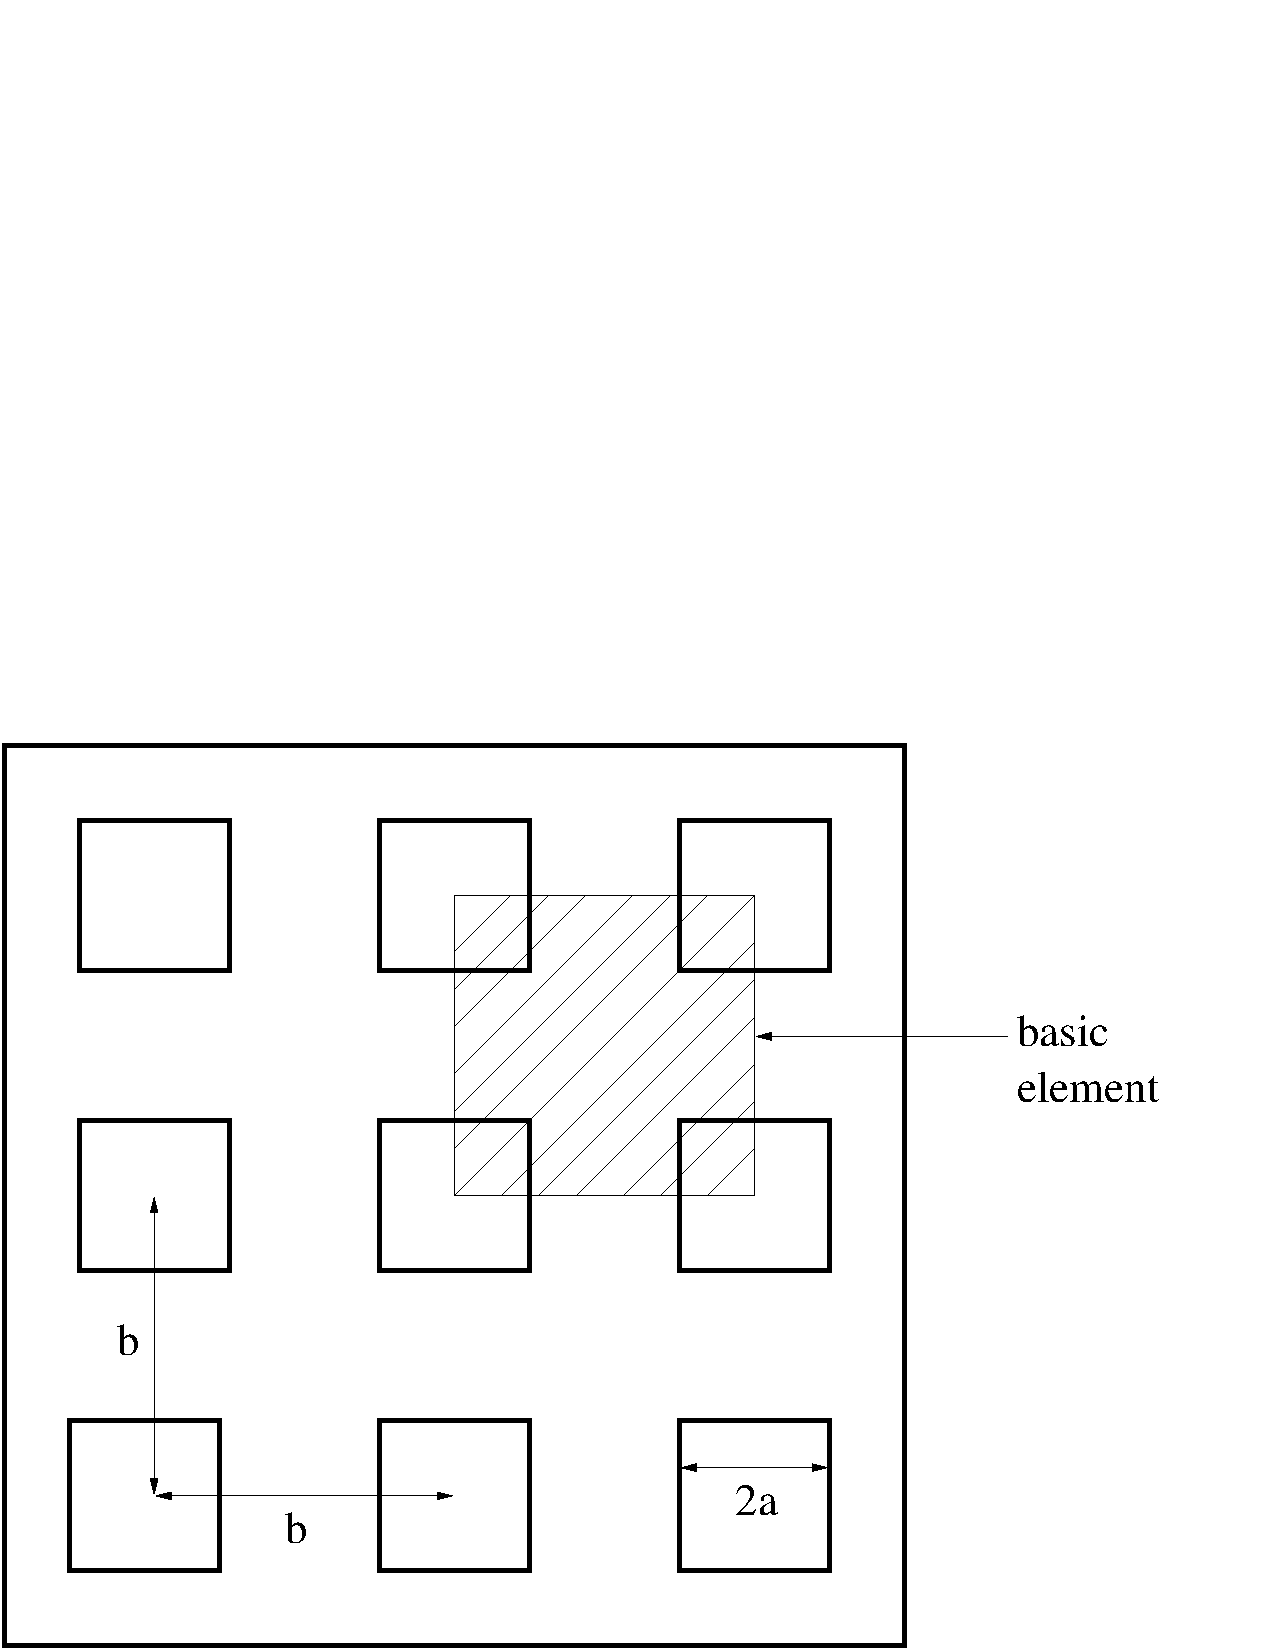
\includegraphics[width=0.6\textwidth]{basic-element}}
\caption{The basic element of the perforated plate consisting of five rectangular
beams}
\label{fg:basic}
\end{figure}

The unit cell of a perforated plate may be assumed to consist of one 
small square plate with side $b-2a$, and of four beams of length $a$ as
shown in Figure~\ref{fg:basic}.
Using approximate formulas an analytical formula for the deformation
energy of the perforated plate is obtained.  
This has to be equal to the deformation energy of 
an unperforated ortoropic membrane. From this condition we get a set of equations
from which the effective parameters may be solved.

The elasticity tensor has three independent components, 
$C_{11}=C_{22}, C_{12}=C_{21}$, and $C_{44}$. 
The expressions for these are
~\cite{pedersen1},
\begin{eqnarray}
C_{11} & = & C_{22} = \frac{E}{b^{2}} \left \{ \frac{b(b-2a)}{1-\nu^{2}} + 
\frac{a(b-2a)^{2}}{b} \right \} \label{eq:C1} \\
C_{12} & = & C_{21} = \frac{\nu E (b-2a)}{b(1- \nu^{2})} \label{eq:C2} \\
C_{44} & = & \frac{E}{4b^{2}(1+ \nu)} \left \{ 2b(b-2a) + \frac{12 K a(b-2a)}{bh^{3}} 
\right\}. \label{eq:C3}
\end{eqnarray} 
where $K$ is a constant\footnote{In article~\cite{pedersen1} there is an error in the definition of
$K$. In the article there is an expression $(b-2a)/h^{3}$, which would make $K$ 
discontinuous at $h=b-2a$.}, 
defined as
\begin{equation}
K= \left \{ \begin{array}{ll}
\frac{1}{3} \left (1-0.63 \frac{b-2a}{h} \right)(b-2a)^{3}h, \quad \mbox{jos  }h>b-2a \\
\frac{1}{3} \left (1-0.63 \frac{h}{b-2a} \right)(b-2a)h^{3}, \quad \mbox{jos  }h<b-2a.  
\end{array}
\right.
\end{equation}

The midplane tension of the perfomarated plate may be reduced to 
lateral stresses of the ortotropic plate by a simple scaling, 
\begin{equation}
 T = \sqrt{(1-4a^{2}/b^{2})} \, T_0 , \label{eq:sigmared}
\end{equation}
where is the tension $T_0$ of the perforated plate. Using this reduced tension and
the modified material parameters of equations~(\ref{eq:C1}),~(\ref{eq:C2}) and~(\ref{eq:C3}) 
the ortoropic plate mimics the behavior of the perforated plate 
when looking at macroscopic quantities. However, the model is not suitable for approximating
maximum stresses around the holes, for example.

\section{Keywords}
\end{versiona}

\sifbegin
\sifitemnt{Solver}{solver id}
\sifbegin
\sifitemnt{Equation}{String SmitcSolver}
\sifitem{Procedure}{File "Smitc"\ "SmitcSolver"}
The procedure which inludes the linear plate model.
\sifitem{Variable}{String Deflection}
This may be of any name as far as it is used consistently also elsewhere.
\sifitem{Variable DOFs}{Integer 3}
Degrees of freedom for the deflection. 
The first degree is the displacment and the two following ones
are its derivatives in the direction of the coordinate axis.
\sifitem{Eigen Analysis}{Logical}
Also the eigenvalues and eigenmodes of the elasticity equation may be computed.
This is done automatically by calling a eigensolver after the original equation has been solved.
The default is \texttt{False}.
\sifitem{Eigen System Values}{Integer}
If the eigenvalues are computed this keyword gives the number of eigenmodes
to be computed. The lowest eigenvalues are always solved for.
\sifitem{Hole Correction}{Logical} 
If the plate is perforated the holes may be taken into account by 
a homogenized model. This is activated with this keyword.
The default is \texttt{False}.
\sifitemnt{Procedure}{File "Smict"\ "SmitcSolver"}
\sifend

\sifitemnt{Material}{mat id}
\sifbegin
\sifitem{Density}{Real}
Density of the plate.
\sifitemnt{Poisson ratio}{Real}
\sifitem{Youngs modulus}{Real}
The elastic parameters are given with Youngs modulus and Poisson ratio.
\sifitem{Thickness}{Real}
Thickness of the plate.
\sifitem{Tension}{Real}
The plate may be pre-stressed.
\sifitemnt{Hole Size}{Real}
\sifitem{Hole Fraction}{Real}
If \texttt{Hole Correction} is \texttt{True} the solver 
tries to find the size and relative fraction of the holes. 
If these are present the hole is assumed to be a square hole.
\sifend

\sifitemnt{Boundary Condition}{bc id}
\sifbegin
\sifitem{Deflection i}{Real}
Dirichlet BC for the components of the deflection, i=1,2,3.
\sifend

\sifitemnt{Body Force}{bf id}
\sifbegin
\sifitem{Pressure}{Real}
Possibility for a body forces. For coupled systems there is a 
possibility to have up to three forces. The two others are then
marked with \texttt{Pressure B} and \texttt{Pressure C}.
\sifitem{Spring}{Real}
The local spring which results to a local force when multiplyed
by the displacement.
\sifitem{Damping}{Real}
The local damping which results to a local force when multiplyed
by the displacement velocity. The spring and damping may also be 
defined as material parameters.
\sifend

\sifend


\begin{versiona}
\bibliography{elmerbib}
\bibliographystyle{plain}
\end{versiona}


\graphicspath{{./}{vonkarman/}}
\Chapter{Elastic Plates}

\modinfo{Module name}{VonKarmanSolve}
\modinfo{Module subroutines}{VonKarmanSolver}
\begin{versiona}
\modinfo{Module authors}{Mikko Lyly}
\modinfo{Document authors}{Mikko Lyly}
\modinfo{Document created}{February 18th 2002}

%\newcommand{\Div}{\nabla\cdot}

\section{Introduction}

\section{Theory}

Given the body force $f=(f_1,f_2)$, pressure $g$, and moment
$h=(h_1,h_2)$, the displacement $u=(u_1,u_2)$, deflection $w$,
and rotation $\theta=(\theta_1,\theta_2)$, of a von Karman-Reissner-Mindlin
plate $\Omega \subset R^2$ is obtained from the equilibrium equations
\begin{eqnarray}
-\Div n & = & f \hskip5truemm (\mathrm{membrane \ force}) \\
-\Div(q + n\cdot \nabla w) & = & g \hskip5truemm (\mathrm{shear \ force}) \\
-\Div m - q & = & h \hskip5truemm (\mathrm{bending \ moment}) 
\end{eqnarray}
the kinematic equations
\begin{eqnarray}
\varepsilon & = & {1\over 2}(\nabla u^T + \nabla u + \nabla w \otimes \nabla w) 
\hskip5truemm (\mathrm{membrane \ strain}) \\
\gamma & = & \nabla w - \theta \hskip15truemm (\mathrm{shear \ strain}) \\
\kappa & = & {1\over 2}(\nabla \theta^T + \nabla \theta) 
\hskip5truemm (\mathrm{curvature}) 
\end{eqnarray}
and the constitutive equations
\begin{eqnarray}
n & = & \mathcal E : \varepsilon \hskip5truemm (\mathrm{membrane \ rigidity}) \\
q & = & \mathcal G \cdot \gamma \hskip5truemm (\mathrm{shear \ rigidity}) \\
m & = & \mathcal K : \kappa \hskip5truemm (\mathrm{bending \  rigidity}) 
\end{eqnarray}
where $\mathcal E$, $\mathcal G$, and $\mathcal K$, are elasticity tensors.
For homogeneous isotropic materials the tensors are defined by the equations
\begin{eqnarray}
\mathcal E : \varepsilon &=& 2Gt \left( \varepsilon 
+ {\nu\over 1-2\nu}(\mathrm{tr}\varepsilon) I \right) \hskip5truemm  \\
\mathcal G \cdot \gamma &=& Gt \gamma \hskip5truemm  \\
\mathcal K : \kappa &=& {Gt^3\over 6}\left( \kappa + {\nu\over 1-\nu}
(\mathrm{tr}\kappa) I\right) \hskip5truemm 
\end{eqnarray}
where $G$ is the shear modulus, $\nu$ is the Poisson ratio, and $t$
is the thickness of the plate. Note that $G=E/[2(1+\nu)]$, where $E$
is the Young modulus.

The solution of the system (1)-(9) minimizes the total potential energy
\begin{equation}
{1\over 2}\int_\Omega (n:\varepsilon + q\cdot\gamma + m:\kappa ) \ d\Omega
- \int_\Omega (f\cdot u + gw + h\cdot\theta) \ d\Omega
\end{equation}
In the finite element solution the non-linear membrane strain enery
term $n:\varepsilon$ is linearized by Newton's method and discretized
by standard Galerkin's method. The shear energy term $q\cdot\gamma$ is
treated by appropriate stabilization and mixed interpolation techniques [1].
The bending energy term $m:\kappa$ is by Galerkin's method without numerical
modifications.

\end{versiona}

\section{Keywords}

\sifbegin
\sifitemnt{Solver}{solver id}
\sifbegin
\sifitemnt{Equation}{String SmitcSolver}
\sifitem{Variable}{String Deflection}
This may be of any name as far as it is used consistently also elsewhere.
\sifitem{Variable DOFs}{Integer 5}
Degrees of freedom for the deflection. 
The first degree is the displacment and the two following ones
are its derivatives in the direction of the coordinate axis.
\sifitem{Hole Correction}{Logical} 
If the plate is perforated the holes may be taken into account by 
a homogenized model. This is activated with this keyword.
The default is \texttt{False}.
\sifitem{Procedure}{File ''Smict'' ''SmitcSolver''}
The following three keywords are used for output control.
\sifend

\sifitemnt{Material}{mat id}
\sifbegin
\sifitem{Density}{Real}
Density of the plate.
\sifitemnt{Poisson ratio}{Real}
\sifitem{Youngs modulus}{Real}
The elastic parameters are given with Youngs modulus and Poisson ratio.
\sifitem{Thickness}{Real}
Thickness of the plate.
\sifitem{Tension}{Real}
The plate may be pre-stressed.
\sifitemnt{Hole Size}{Real}
\sifitem{Hole Fraction}{Real}
If \texttt{Hole Correction} is \texttt{True} the solver 
tries to find the size and relative fraction of the holes. 
If these are present the hole is assumed to be a square hole.
\sifend

\sifitemnt{Boundary Condition}{bc id}
\sifbegin
\sifitem{Deflection i}{Real}
Dirichlet BC for the components of the deflection, i=1,2,3.
\sifitem{Current Density BC}{Logical}
Must be set to {\tt True} if Neumann BC is used.
\sifitem{Current Density}{Real}
Neumann boundary condition for the current.
\sifend

\sifitemnt{Body Force}{bf id}
\sifbegin
\sifitem{Pressure}{Real}
Possibility for a body forces. For coupled systems there is a 
possibility to have up to three forces. The two others are then
marked with \texttt{Pressure B} and \texttt{Pressure C}.
\sifitem{Spring coefficient}{Real}
The local spring which results to a local force when multiplyed
by the displacement.
\sifitem{Damping coefficient}{Real}
The local damping which results to a local force when multiplyed
by the displacement velocity. The spring and damping may also be 
defined as material parameters.
\sifend

\sifend



\graphicspath{{./}{freesurface2d/}}
\Chapter{Free Surface with Constant Flux}

\modinfo{Module name}{\Idx{FreeSurfaceReduced}}
\modinfo{Module subroutines}{FreeSurfaceReduced}
\begin{versiona}
\modinfo{Module authors}{Peter R�back}
\modinfo{Document authors}{Peter R�back}
\modinfo{Document edited}{August 5th 2002}


\section{Introduction}

The determination of free surface is often an essential part of solving
a fluid dynamics problem. Usually the surface is found by solving a 
free surface equation resulting from force balance, 
or by finding the free surface from zero flux condition.
In some extreme cases both of these methods were found to fail and 
therefore an alternative approach was taken. The method can 
only be applied to stationary 2D or axisymmetric flows where the total flux 
is conserved. This is the case, for example, in many \Idx{coating} and 
\Idx{drawing} processes.


\section{Theory}

\index{mass conservation}
The determination of the free surface takes use of the 
conservation of mass. If the flow is stationary the mass flux through all 
planes cutting the flow must be same.
In the following we concentrate on the axisymmetric case which has more 
applications than the 2D case. 

In the axisymmetric case the mass flux is obtained from 
\begin{equation}
  f(R,z) = \int_{R_0}^{R} (\vec{u}\cdot\vec{n}) \, r ds.
\end{equation}
The free surface is set by finding 
a surface profile $R(z)$ such that the integral is
constant for all nodes on the surface, or 
\begin{equation}
  f(R,z_j) = f(R_1,z_1) \ \ \ \ \forall j \in  [1,M].
\end{equation}
Note that the factor $2\pi$
has been consistently omitted since it has no bearing
to the shape of the free surface.

The subroutine uses simple heuristics to determine the direction 
of the flow on the free surface. The first upwind node $z_1$ on the free surface is 
assumed to be fixed and the corresponding flux is $f_1$.
The new radius is set approximately by assuming that the 
added or removed flow has the same velocity as the 
velocity on the surface.
Then the corrected radius is found from
\begin{equation}
  u_n R^{(m)} \, d R^{m} = f(R^{(m)},z) - f(R_1,z_1)
\end{equation}
or
\begin{equation}
  R^{(m+1)} = R^{(m)} + \frac{f(R^{(m)},z) - f(R_1,z_1)}{u_n R^{(m)}}.
\end{equation}
After the new profile is being found the 
element nodes are moved to the new positions.
The nodes that are not on the surface may be mapped in 
many different ways. The straight-forward strategy is to use linear 1D mapping.
Also more generic 2D mapping may be used.
 
The free surface and the fluid flow must 
be consistent and therefore the system must 
be solved iteratively.
When convergence of the coupled system has been obtained 
the suggested $d R$ vanishes and the free surface solver 
does not affect the solution.

Sometimes the free surface solver overshoots and therefore it may
be necessary to use relaxation to suppress the large 
changes of the solution.

Note that the free surface solver is simple based on mass conservation. No
forces are applied on the free surface. If surface tension needs to be taken 
into account it may be done while solving the Navier-Stoke equation.


\section{Applicable cases and limitations}

The method has some limitations which are inherent of the method:
\begin{itemize}
\item Limited to steady-state simulations.
\item Limited to 2D and axisymmetric cases.
\item If there is back-flow within the free surface flow the correctness of the 
solution is not guaranteed.
\end{itemize}
Some limitations result from the current implementation:
\begin{itemize}
\item The free surface must be oriented so that the flow is on its negative side.
\item There may be several free surfaces of this type but they must be directed
	the same way.
\item The line integral from $R_0$ to $R$ may cause some difficulties in 
	unstructured meshes. Therefore structured meshes are favored.
\item At the moment density is assumed to be constant and
 	therefore only incompressible fluids may be considered.
\end{itemize}



\section{Keywords}
\end{versiona}

\sifbegin
\sifitemnt{Solver}{solver id}
\sifbegin
\sifitemnt{Equation}{String "Free Surface Reduced"}
\sifitem{Variable}{String dx}
The change in the free surface coordinate.
This may be of any name as far as it is used consistently also elsewhere.
\sifitem{Variable DOFs}{Integer 1}
Degrees of freedom for the free surface coordinate.
\sifitem{Procedure}{File "FreeSurfaceReduced"\ "FreeSurfaceReduced"}
The following four keywords are used for output control.
\sifitem{Perform Mapping}{Logical}
If this keyword is {\tt True} the coordinate 
mapping is done locally by using linear 1D mapping.
This is also the default. 
Also 2D mapping is possible by using a separate 
mesh update solver. Then the keyword should be set to \texttt{False}.
\sifitem{Nonlinear System Relaxation Factor}{Real}
The changes in the free surface may be relaxed. The 
default is no relaxation or value 1.0

\sifitem{Nonlinear System Convergence Tolerance}{Real} 
This keyword gives a criterion to
terminate the nonlinear iteration after the maximum change in the 
free surface coordinate is small enough
\begin{equation}
 \max || d R / ( R - R_0 ) ||  < \epsilon  \nonumber
\end{equation}
where $\epsilon$ is the value given with this keyword.
\sifend

\sifitemnt{Boundary Condition}{bc id}
\sifbegin
\sifitem{Free Surface Reduced}{Logical}
Must be set to {\tt True} for the free surface when the solver is used.
The boundary must be simply continuous.
\sifitem{Free Surface Number}{Integer}
If more than one free surface of the reduced type is present simultaneously
they must somehow be separated. This keyword is for that purpose.
The surfaces should be ordered from 1 to the number or free surfaces.
Value 1 is also the default if the surface is active.
Note that free surfaces with different numbers should be aligned the same way and should 
not touch each other.
\sifitem{Free Surface Bottom}{Logical}
If this flag is free it sets the lower boundaries of integration 
when solving for the free surface. Note that this surface should not touch any of the 
free surfaces. A free surface is automatically a lower boundary for another 
free surface.
\sifend
If mapping is not performed within the solver also boundary conditions
for the mapping are required. Surface tension may be taken into account 
while solving the Navier-Stokes equation. The proper keywords for 
activating the surface tension are explained in the manual of the Navier-Stokes solver.
\sifend



%\bibliography{elmerbib}
%\bibliographystyle{plain}



\graphicspath{{./}{levelset/}}

\chapter{Level-Set Method}\label{Level-Set}

\modinfo{Module name}{\Idx{LevelSet}}
\modinfo{Module subroutines}{\Idx{LevelSetSolver}, \Idx{LevelSetDistance}, \Idx{LevelSetIntegrate}, 
\Idx{LevelSetCurvature}, \Idx{LevelSetTimestep}}
\modinfo{Module authors}{Peter R�back, Juha Ruokolainen}
\modinfo{Document authors}{Peter R�back}
\modinfo{Document created}{5.4.2006}
\modinfo{Document edited}{28.4.2006}

 
\section{Introduction}

There are a number of problems involving \Idx{free surface}s in continuum mechanics.
There are two main strategies to solve them using the finite element method:
\Idx{Lagrangian} and \Idx{Eulerian} approach. 
In the Lagrangian approach the free surface is solved exactly so that 
it is also an interface between the individual elements. This 
requires that the computational mesh is distorted in a way that 
this is possible. However, often the changes in geometry may be too drastic or
even the whole topology may change and the Lagrangian approach is no longer feasible.
The Eulerian approach describes the interface in a fixed mesh using 
some additional variable to describe the position of the interface. 
One possible Eulerian technique is the \Idx{level-set method} (LSM). 

In the level-set method the free surface is given as a zero level-set of a
higher dimensional variable. E.g. for 2D surfaces the level-set function is 
defined in 3D space. The level-set function is usually defined to be a \Idx{signed distance} 
so that inside the domain it obtains a positive value and outside a negative value.
The changes in the value of the level-set function mean also that 
the interface changes the position. 

This module includes several different subroutines that may be used 
when applying the level-set method.
Currently there is no \Idx{reinitialization} strategy for 3D problems. Also some 
other procedures are not fully optimized for the best performance. Therefore
the current implementation is best applied to quite simple 2D problems.


\section{Theory}

The interface is defined by a marker function $\phi$ so that 
at the interface $\phi=0$, inside the fluid of interest $\phi > 0$ and
elsewhere $\phi < 0$. The interface is update by solving the equation
\begin{equation}
\Der{\phi}{t} + \Vec{u} \cdot \nabla \phi = a
\label{eq:levelset1}
\end{equation}
where $\Vec{u}$ is the convection field and $a$ is the normal 
flux on the interface. 
It is quite challenging to solve the differential equation above
without diffusion effects playing a significant role. It is advisable to
use 2nd order time-discretization schemes and short timesteps. 
More precisely, the Courant number $C=|\vec{u}|dt/h$ should be below unity.

It is desirable that the absolute value of function equals the shortest 
distance to the zero level-set. However, as the level-set function 
is advected this property may be gradually lost. Therefore a process called 
reinitialization may be evoked. In 2D the reinitialization may be easily done 
by geometric procedure. First the zero level-set is formed by going through all
the elements and finding the line segments that make the zero level-set. Then 
the minimum distance of all the nodes is computed by a brute-force search.  
Assuming there are $N$ nodes and $M$ line segments the search algorithm is 
$N\times M$ which is quite acceptable complexity for small cases but 
may become computationally costly in large cases.

The line segments may be assumed to go with the flow and thereby 
they form an on-the-fly Lagrangian mesh. 
Therefore it is also possible to advect the line segments when the velocity 
field is given since for any node $\Vec{r} =\Vec{r} + \Vec{u}\,dt$.
After the advection the shortest distance is
computed. In the case of no advection the sign of the distance is inherited from the 
original level-set function. However, when the level-set is also convected the
sign must be deduced from the geometric information as well. In the current
implementation each line segment is given a flag telling on which side of the element
the fluid of interest is located. This directional information is then used in giving the
correct sign for the distance.

The volume of the fluid of interest in the level-set method may be 
computed over an integral that obtains a value one inside the fluid and 
value zero outside the fluid. The \Idx{Heaviside function} 
$H(\phi)$ has this desired property.
However, as the interface does not 
follow the element division the numerical integration 
would result into spurious fluctuations depending on the position of the interface
within the elements. To obtain a smooth behavior the 
Heaviside function must be regularized:
\begin{equation}
  H_\alpha(x) = \begin{cases} 
    0, & x < \alpha \\
    \frac{1}{2}\left(1+\sin \left(\frac{x}{a}\frac{\pi}{2} \right) \right), & |x| \leq \alpha \\
    1, & x > \alpha , 
  \end{cases}
\end{equation}
where $\alpha$ is the interface bandwidth which equals typically the size of a few elements.
Now the volume (area in 2D) is obtained by the integral
\begin{equation}
  V = \int_\Omega H_\alpha (\phi) \, d\Omega .
  \label{eq:levelsetvolume}
\end{equation}
After the same regularization the area (length in 2D) may be obtained from the 
integral
\begin{equation}
  A = \int_\Omega \delta_\alpha (\phi)|\nabla\phi|  \, d\Omega
  \label{eq:levelsetarea}
\end{equation}
where the \Idx{delta function} is 
\begin{equation}
  \delta_\alpha(x) = \begin{cases} 
    0, & |x| > \alpha \\
    \frac{1}{2\alpha} \cos \left ( \frac{x}{a}\pi \right), & |x| \leq \alpha. 
  \end{cases}
\end{equation}

The information obtained by the above integrals may be used to improve the 
volume conservation of the level-set advection. If the initial volume $V_0$ is known
the level-set function may be given a small correction by 
\begin{equation}
  d\phi = \frac{V_0 - V}{A}.
  \label{eq:levelsetcorrect}
\end{equation}
This correction has no physical basis but it may be argued that a consistently
small update of the level-set function has a minor effect in overall results. 
It is more important that the volume is conserved since the 
history information of the shape of a bubble is 
gradually lost while the errors in volume are never forgotten. However, if the 
fluid of interest is divided into several parts this kind of overall correction
does not have any justification since it could ruin the volume 
balance between the different domains.

The problems in accuracy may be partially resolved by using an optimal 
timestepping strategy. This may be achieved by looking at the velocity field 
around the active boundary. The normal velocity may be obtained by 
$u_n=\Vec{u}\cdot\nabla\tilde{\phi}$. Registering the maximum velocity at 
band the timestep may be limited so that the Courant number is bound.
If $ds$ is the maximum allowed change in the 
position of the zero level-set the corresponding time-step is
$dt = ds / \max |u_n|$. 

In the Eulerian approach to the free surface 
problems the \Idx{surface tension} force must be smeared out to a volume force
within a narrow band from the interface. The transformation is achieved by 
using a regularized delta function,
\begin{equation}
  \int_\Gamma \sigma \kappa \, d\Gamma = \int_\Omega \sigma \kappa \delta(\phi) 
  \nabla \phi \, d\Omega,
\end{equation}
where $\sigma$ is the surface tension
coefficient and $\kappa$ the \Idx{curvature} of the interface given by 
\begin{equation}
  \kappa = \nabla \cdot \frac{\nabla \phi}{|\nabla \phi|}.
\end{equation}
In the finite element approach the force cannot be estimated directly since
it involves three derivatives of the level-set function. Therefore we must solve
an additional equation for the \Idx{curvature} $\kappa$,
\begin{equation}
  \kappa - c_\kappa \nabla^2 \kappa = \nabla \cdot \nabla \tilde{\phi} .
  \label{eq:levelsetcurvature}
\end{equation}
Here $c_\kappa$ is an ad'hoc diffusion coefficient that may be used to 
smooth the resulting curvature field.
Otherwise the sharp corners may result to very large peak values of the 
curvature. 
The weak formulation of the above equation introduces surface fluxes 
which are evaluated from the normal derivatives of the level-set function.
Once the level-set function and the corresponding curvature have been computed 
the surface tension may be applied as a volume force in the flow equations. 


\section{Keywords}

\subsection*{LevelSetSolver}

This subroutine uses the finite element method to solve the equation
(\ref{eq:levelset1}). The implementation is valid in 2D, 3D and axisymmetric 
problems.

\sifbegin
\sifitemnt{Solver}{solver id}
\sifbegin
\sifitemnt{Equation}{String "Level Set Solver"}

\sifitem{Procedure}{File "LevelSet"\ "LevelSetSolver"}
The subroutine for advecting the level-set function.

\sifitem{Variable}{String "Surface"}
The name of the level-set function. This may be chosen freely as long as it is used
consistently elsewhere.

\sifitem{Stabilize}{Logical}
Either stabilization or bubbles are used to solve the convection problem. This
flag enforces the stabilization on. 
\sifend

\sifitemnt{Material}{mat id}
\sifbegin
\sifitemnt{LevelSet Velocity 1}{Real}
\sifitemnt{LevelSet Velocity 2}{Real}
\sifitem{LevelSet Velocity 3}{Real}
The velocity field that advects the level-set function. This may be a constant field or also 
something computed with the Navier-Stokes solver. 
\sifend

\sifitemnt{Body Force}{bodyforce id}
\sifbegin
\sifitem{LevelSet Flux}{Real}
The flux (i.e. the normal velocity) of the level-set function. 
\sifend
\sifend


\subsection*{LevelSetDistance}

This solver uses the geometric information to compute the signed distance
and, if desired, to advect the zero level-set at the same time.
This solver does not solve an equation and hence it does not need to have a 
variable of its own. The solver is limited to 2D and axisymmetric cases.

\sifbegin
\sifitemnt{Solver}{solver id}
\sifbegin
\sifitemnt{Equation}{String "Level Set Distance"}

\sifitem{Procedure}{File "LevelSet"\ "LevelSetDistance"}
The subroutine for renormalizing (and advecting) the level-set function.

\sifitem{LevelSet Variable}{String "Surface"}
This keyword should refer to the name of the level-set variable that 
is used to advect the field. The default is \texttt{Surface}.

\sifitem{Exported Variable 1}{String "Surface"}
In case the level-set variable does not exist it must be introduced.
This may be the case if this subroutine is also used for advecting the 
level-set function.

\sifitem{LevelSet Convect}{Logical}
Whether to also convect the level-set function.
Default is \texttt{False}.

\sifitem{Extract Interval}{Integer}
When this function is used to extract the zero level-set function the 
user may choose the interval how often this is done. The default is 
one. Just extracting the level-set may be useful if one just wants to save
the zero level-set without activating reinitialization.

\sifitem{Reinitialize Interval}{Integer}
When this function is used to reinitialize the level-set function the 
user may choose the interval how often this is done. The default is 
one but often this results to excessive smoothening of the level-set field. 
If reinitialization is asked the zero level-set will also be automatically extracted.

\sifitem{Reinitialize Passive}{Logical}
If this keyword is set \texttt{True} the reinitialization is not applied to the level-set field.
The field is only used to extract the zero level-set and compute the corresponding signed distance 
but this information is not used to change the original field.

\sifitem{Narrow Band}{Real}
In case that also the convecting is done by this solver there is the possibility to introduce 
a narrow band which gives the distance at within the level-set function is recomputed. 
Default is $\infty$. Typically this should be larger that 
the level-set bandwidth $\alpha$ used to evaluate surface integrals.

\sifitem{Filename}{File}
The zero level-set may also be saved. It consists of a number of line segments that are
defined elementwise. The results from the file may be used for visualization, for example,
in MatLab. If no filename is given the zero level-set is not saved. 

\sifitem{File Append}{Logical}
If the above is given this flag enforces the results to be appended on the same 
file rather than writing over the old results.
\sifend

\sifitemnt{Material}{mat id}
\sifbegin
\sifitemnt{LevelSet Velocity 1}{Real}
\sifitem{LevelSet Velocity 2}{Real}
If also convection is accounted in this solver the convection field
is given by the above expressions. Currently it is not possible to give the desired 
surface flux as it is not uniquely defined for the line segments having different normals
even at the same point.
\sifend
\sifend


\subsection*{LevelSetIntegrate}

This subroutine computes the integrals (\ref{eq:levelsetvolume}) and 
(\ref{eq:levelsetarea}).  
In addition of computing volume and surface integrals this
subroutine may also be used to set the absolute level of the level-set function
so that volume is conserved using equation (\ref{eq:levelsetcorrect}).
The implementation is valid in 2D, 3D and axisymmetric 
problems.

\sifbegin
\sifitemnt{Solver}{solver id}
\sifbegin
\sifitemnt{Equation}{String Level Set Integrate}

\sifitem{Procedure}{File "LevelSet"\ "LevelSetIntegrate"}
The subroutine for computing the integrals.

\sifitem{LevelSet Variable}{String "Surface"}
This keyword gives the name of the level-set function used for computing the 
integrals. The default is \texttt{Surface}.

\sifitem{LevelSet Bandwidth}{Real}
When computing the values over the domain the interface is treated a 
with smooth functions. How smooth the functions are depends on the
value of this keyword. Typically the bandwidth should be such that the 
interface is extended over a few elements. 

\sifitem{Conserve Volume}{Logical}
The volume in the level-set formulation is not conserved by construction. 
To that end the level of the level-set function may be tuned so that 
conservation is enforced. The default is \texttt{False}. 

\sifitem{Conserve Volume Relaxation}{Real}
If conservation is enforced it may be done only partially as there are
inaccuracies in the avalution of the volume integrals. The default is one.

\sifitem{Initial Volume}{Real}
If conservation is enforced the target volume is given by this keyword.
Otherwise the volume from the first timestep is used as the target value.

\sifend
\sifend



\subsection*{LevelSetCurvature}

This solver computes the value of the curvature give the level-set function using
equation (\ref{eq:levelsetcurvature}).

\sifbegin
\sifitemnt{Solver}{solver id}
\sifbegin
\sifitemnt{Equation}{String Level Set Curvature}

\sifitem{Procedure}{File "LevelSet"\ "LevelSetCurvature"}
The subroutine for computing the curvature.

\sifitem{Variable}{String "Curvature"}
The name of the curvature variable.

\sifitem{LevelSet Variable}{String "Surface"}
This keyword gives the name of the level-set function used for computing the 
integrals. The default is \texttt{Surface}.

\sifitem{Curvature Diffusion}{Real}
Artificial diffusion may be used to control the singularities of the 
curvature field around sharp corners. The default is zero.

\sifitem{Curvature Coefficient}{Real}
A constant that is used to multiply the curvature field before the solver is 
exited. This may be used for example to change the sign of the curvature if the 
material of interest is on the outside and not an the inside.

\sifitem{LevelSet Bandwidth}{Real}
The delta function for the volume force may be applied to the curvature field also within this 
solver directly. This has the disadvantage that the evaluation is done at nodal points 
rather than at the integration points. However, if the flow solver used may not be modified this 
may be the best alternative. If this keyword does not exist, no delta function is used to 
filter the curvature field. 

\sifend

\sifitemnt{Boundary Condition}{bc id}
\sifbegin
\sifitem{Levelset Curvature BC}{Logical}
The weak formulation of the curvature computation results to boundary integrals that should be set
at all surfaces where the curvature is computed.
\sifend
\sifend


\subsection*{LevelSetTimestep}

The solution of the level-set function is accurate only if 
the timestep is limited so that the local Courant number along the zero level-set
is in the order of one or smaller. 
A tailored function for setting the timestep is given in this module.
This solver assumes that the
level-set variable is named \texttt{Surface} and that this variable is related to 
some solver. The velocity needed for setting the timestep should be given by the 
keywords \texttt{LevelSet Velocity i}, where \texttt{i=1,2,3}.

\sifbegin
\sifitem{Simulation}{}
The function call and the needed parameters reside in the \texttt{Simulation} block
of the command file.

\begin{verbatim}
Timestep Function 
  Real Procedure "LevelSet" "LevelSetTimestep"
\end{verbatim}
%
\sifbegin
\sifitem{LevelSet Courant Number}{Real}
This keyword gives the desired Courant number of for the level-set 
solvers. The default for the desired Courant number is one. 

\sifitem{LevelSet Timestep Directional}{Logical}
If the timestep limit is active this option may be used to account only the normal
direction of the interface velocity rather that the absolute direction. 
Default is \texttt{False}. 

\sifend
\sifend


%\bibliography{elmerbib}
%\bibliographystyle{plain}



% Utility solvers - No new physics

\graphicspath{{./}{rigidbody/}}
\Chapter{System Reduction for Displacement Solvers}

\modinfo{Module name}{\Idx{RigidBodyReduction}}
\modinfo{Module subroutines}{RigidBody}

\begin{versiona}
\modinfo{Module authors}{Antti Pursula}
\modinfo{Document authors}{Antti Pursula}
\modinfo{Document edited}{August 27th 2003}


\section{Introduction}

\index{reduced order model} This module is used to reduce and simplify
the computation of a displacement solver when the problem includes
rigid blocks. In such a case, it is often difficult for iterative
solvers to find a solution for the full system, and direct solvers
become obsolite when the system is large enough. The convergence and
also the speed of the solution can be substantially improved when the
degrees of freedom corresponding to the nodes belonging in the rigid
blocks are reduced onto the 6~DOFs (3~in~2D) of the corresponding
rigid body. In the module, the reduction is achieved via a
\Idx{projection matrix}.

Additionally, the routine automatically eliminates the degrees of
freedom corresponding to the Dirichlet boundary conditions. It is also
possible to request the elastic regions to be extended into the rigid
blocks. There is also possibility to reorder the reduced matrix
elements to decrease its bandwidth. 


\section{Theory}

The module starts with normally constructed matrix equation for the
unknown displacements $x$, $Ax=b$. Let us assume that the nodes are
ordered in such a way that the first $n$ elements of the vectors
correspond to the elastic parts of the structure and the remaining $m$
elements correspond to the rigid parts of the structure. The goal is
to reduce the $(n+m)\times (n+m)$ matrix $A$ to a $(n+\alpha k)\times
(n+\alpha k)$ matrix $B$, where $k$ is~3 for 2D and~6 for 3D problems
and $\alpha$ is the number of rigid blocks present. Reductions are
made also for the vectors so that finally the matrix equation reads
$Bu = f$.

The relation between the unknowns is 
\begin{equation}
x = Pu,
\end{equation}
where the projection matrix $P$ ties the nodes in the rigid bodies to
the same displacements in coordinate directions and the same rotations
about the coordinate axis. The rotations are defined with a coordinate
system whose origin is at the center of each rigid body.  For the right
hand sides we can write
\begin{equation}
f = Qb,
\end{equation}
where the matrix $Q$ sums the forces and torques present at the nodes
in rigid bodies for a resultant force and torque of the center point
of the corresponding rigid body. In both mappings, the rotations are
linearized so the module is valid only for cases where the rotations
are small.

Using these definitions, we have
\begin{equation}
Ax=APu=b
\end{equation}
and
\begin{equation}
Bu=f=Qb.
\end{equation}
Combining the equations gives $Bu=QAPu$ and thus
\begin{equation}
B = QAP.
\end{equation}
With a suitable order of the rotations one can write 
\begin{equation}
Q=P^T \equiv C,
\end{equation}
and
\begin{equation}
B = CAC^T.
\end{equation}
The matrix $C$ has a identity matrix block of size $n\times n$ which
keeps the elastic nodes intact, and a projection block of size
$\alpha k\times m$. 

The reduced order solution $u$ is transformed back to the original
nodes by the same mapping
\begin{equation}
x=C^T u.
\end{equation}


\section{Applicable cases and limitations}

The module works for
\begin{itemize}
\item Linear steady-state problems
\item Linear transient problems
\item Eigen analysis
\item Quadratic eigenproblems
\end{itemize}
%
There are following limitations:
\begin{itemize}
\item Rigid blocks should not have common nodes (there should be
elastic nodes in between rigid blocks)
\item If a Dirichlet bc is given on a node of a rigid block then the
entire rigid block is assumed to be fixed in all directions
\end{itemize}



\section{Keywords}
\end{versiona}

\sifbegin
\sifitemnt{Body}{body id}
\sifbegin
  \sifitem{Rigid Body}{Logical}
Value {\tt True} defines the rigid body.
\sifend
\sifitem{Solver}{solver id}
The module does not need a separate solver but
a call in the stress analysis,
or the elasticity solver in the linear mode. 
\sifbegin
\sifitemnt{Equation}{String Stress Analysis}
\sifitemnt{Variable}{String Displacement}
\sifitem{Variable DOFs}{Integer}
It is important to give the DOFs right, either 2 or 3 depending on
the dimension.
\sifitem{Before Linsolve}{File "RigidBodyReduction"\ "RigidBody"}
The model order reduction is performed after the matrix has been assembled
but before the matrix equation has been solver. The matrix equation is 
modified to a smaller equation and the new equation is solved within the subroutine.
\sifitem{Eigen Analysis}{Logical}
It is possible to use the model order reduction with modal analysis, as
well as with static and transient cases.
\sifitem{Eigen System Values}{Integer}
The number of eigen values to be computed.
\sifitemnt{Eigen System Damped}{Logical}
\sifitem{Eigen System Use Identity}{Logical [True]}
The reduction is possible also with quadratic (damped) eigenproblems.
\sifitem{Optimize Matrix Structure}{Logical}
If true, the matrix structure is optimized. This feature is recommended 
since the reduced matrix has often very scattered structure. The
optimization is performed with the Cutholl-McKee algorithm.
\sifitem{Reverse Ordering}{Logical}
This flag can be used to reverse the matrix ordering if the matrix
structure is optimized, resulting in reverse Cuthill-McKee ordering.
\sifitem{Extend Elastic Region}{Logical}
If true, the elastic regions of the geometry are extended into the rigid 
block. This feature allows taking into account the bending in the joints 
between elastic and rigid parts.
\sifitem{Extend Elastic Layers}{Integer}
Defines the number of element layers that the elastic regions are extended.
\sifitem{Output Node Types}{Logical}
Writes in the ElmerPost output file a variable describing the status of 
each node in the geometry. The variable has value 0 for elastic nodes,
-1 for rigid blocks that are fixed due to a Dirichlet boundary condition,
and a positive integer for separate rigid blocks. The variable may be 
used to check that the reduction is performed on the right blocks, and to
check how many layers the elastic regions should be extended, for example.
\sifitem{Additional Info}{Logical}
If true, additional information is written about the performed tasks
during the simulation. 
\sifend
\sifend


\begin{versiona}
\section{Examples}

\begin{figure}[tbhp]
  \vspace{-25mm}
  \centerline{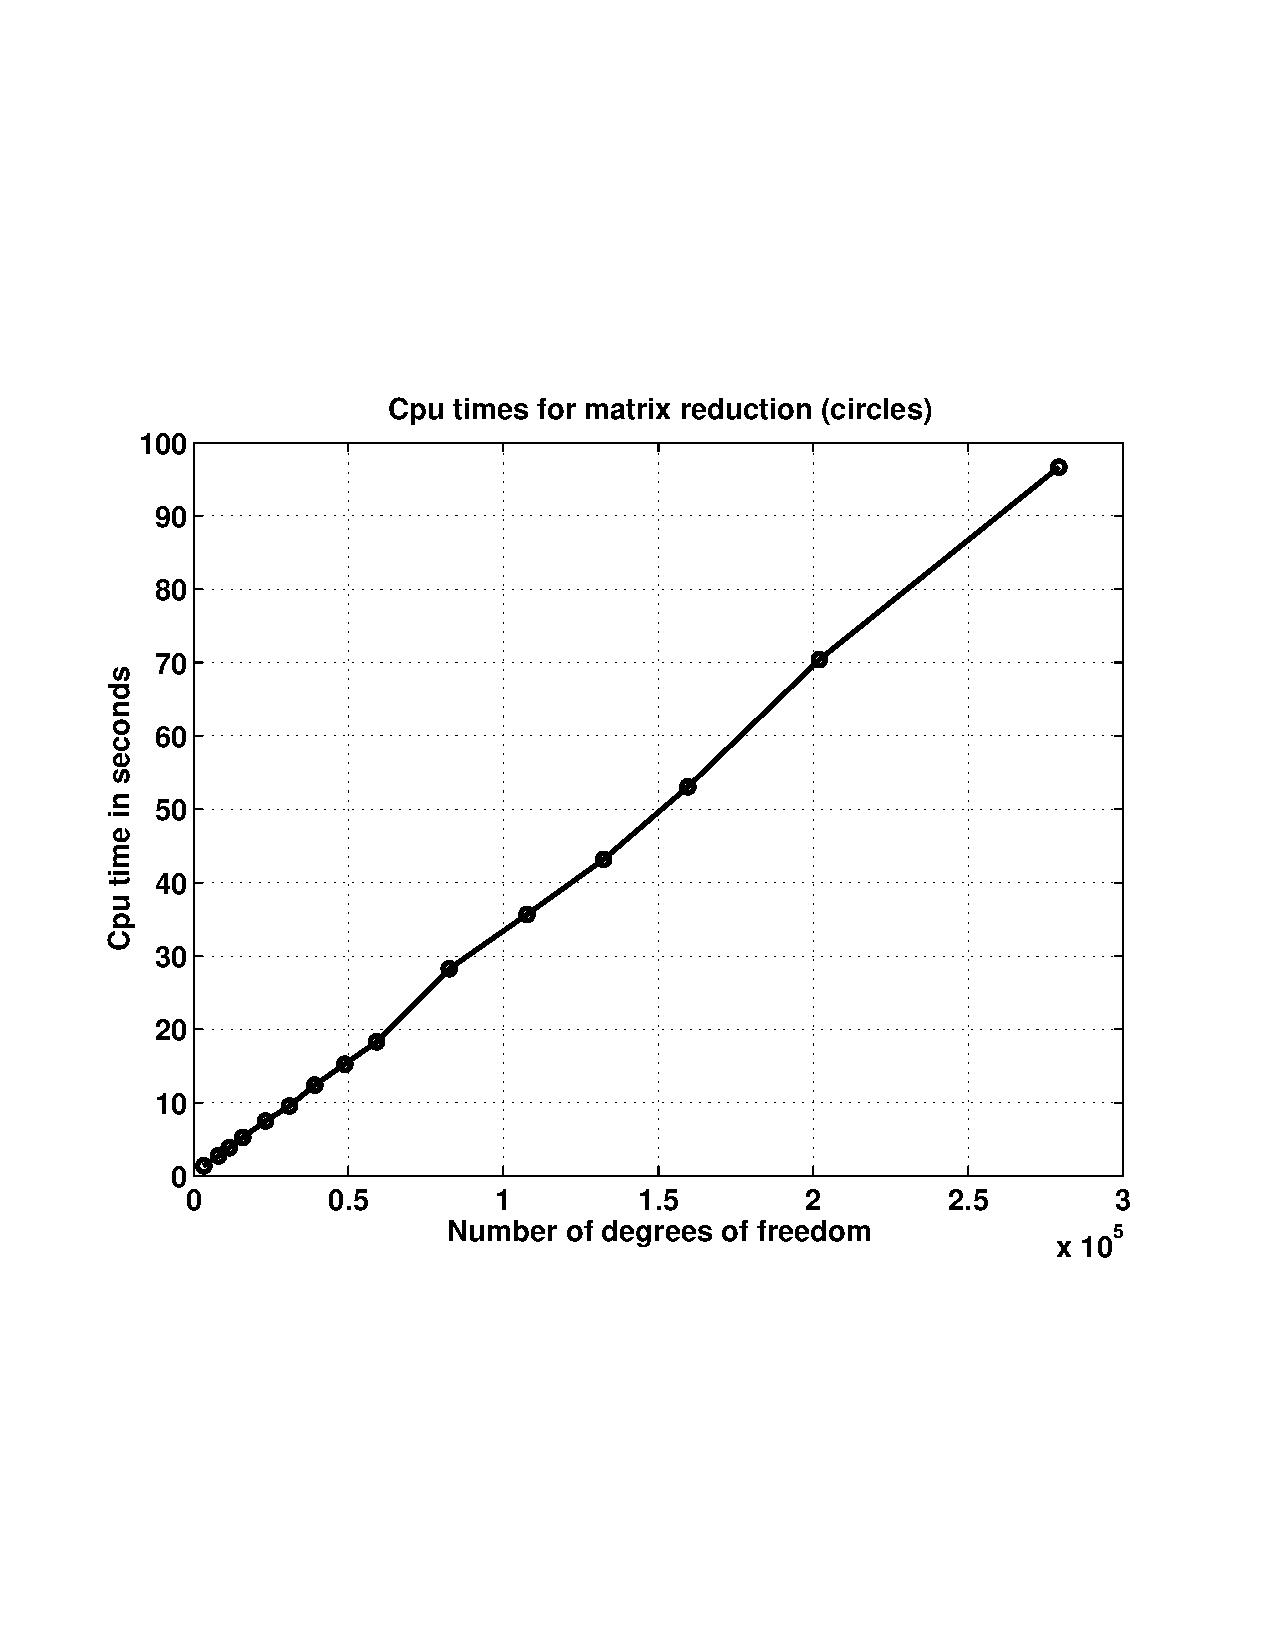
\includegraphics[width=0.6\textwidth]{reduction_cpu.pdf}}
  \vspace{-25mm}
  \caption{The cpu time required for the matrix reduction operations
  depends linearly on the degrees of freedom in the system.}
\end{figure}

%\begin{figure}[tbhp]
%  \centerline{\includegraphics[width=0.5\textwidth]{modes.ps}}
%  \caption{Two eigenmodes (1st and 5th) of a supported structure
%  calculated using matrix reduction.}
%\end{figure}

\end{versiona}


\graphicspath{{./}{moving_elstat/}}
\chapter{Electrostatics of moving rigid bodies}\label{Electrostatics}

\modinfo{Module name}{\Idx{MovingElstatSolver}}
\modinfo{Module subroutines}{\Idx{MovingElstatSolver}}
\begin{versiona}
\modinfo{Module authors}{Peter R�back}
\modinfo{Document authors}{Peter R�back}
\modinfo{Document created}{26.1.2006}
\modinfo{Document edited}{17.5.2006}


\section{Introduction}

\index{rigid body movement}
This solver is tailored for solving electrostatic problems that 
occur in the movement of rigid bodies in respect to one another. 
Here the movement is assumed to be a combination of rotations and 
translations. We are mostly interested in lumped quantities. 
The most important quantity is the capacitance of the moving body 
at different positions. In addition the sensitivity of the capacitance
and the moment of the electric force may be computed. The information is
saved in a generic tabulated form and also as a lumped circuit model
of Aplac. 

For a more generic cases of the electrostatics and
mesh adaptation the user is encouraged to use the 
existing separate solvers. 


\section{Electrostatics}

Assuming a constant permittivity $\varepsilon$, 
absence of free charges, and non-conducting 
media the equation for the electrostatic potential $\phi$ yields,
\begin{equation}
  -\varepsilon \nabla \cdot \nabla \phi = 0.
\end{equation}
Obviously the constant multiplier may be dropped for convenience.

The energy of the electric field may be computed from
\begin{equation}
  E  = \frac{1}{2}\varepsilon \int_\Omega |\nabla \phi|^2 d\Omega.
\end{equation}
If there is only one potential difference $\Phi$ present then the 
capacitance $C$ may be computed from
\begin{equation}
  C = \frac{2E}{\Phi^2} .
\end{equation} 

The electric force is calculated by integrating the 
electrostatic \Idx{Maxwell stress tensor} over the specified surface. Using
the stress tensor $\overline{\overline T}$ the total force on the
surface $S$ can be expressed as
\begin{equation}
\Vec{F} = \int_S \overline{\overline T}\cdot\Vec{n}\,dS.
\end{equation}
The components of the Maxwell stress tensor for linear medium are
\begin{equation}
T_{ij} = -D_iE_j + \frac{1}{2}\delta_{ij}\Vec{D}\cdot\Vec{E},
\end{equation}
where electric field $\vec{E}$ and electric displacement field
$\vec{D}$ are obtained from 
\begin{equation}
\vec{E} = -\nabla\phi,
\end{equation}
and
\begin{equation}
\vec{D} = -\varepsilon \nabla \phi.
\end{equation}
The moment around a given point $\Vec{r}_0$ is given by,
\begin{equation}
\Vec{F} = \int_S \overline{\overline T}\cdot\Vec{n}\times 
(\Vec{r}-\Vec{r}_0)\,dS.
\end{equation}

One may get an secondary estimation for the capacitance from the integral of the 
surface charges. 
\begin{equation}
  C' = \Inv{\Phi} \int_S \Vec{D} \cdot \Vec{n}\, dS .
\end{equation}
This estimate of capacitance has a much bigger numerical error than the one defined
by the volume integral. However the estimate may be usufull in evaluating the 
accuracy of the capacitance. The volume integral approaches the exact capacitance from
above while the surface integral approaches it from below.  



\section{Mesh movement}

The generic mesh movement of Elmer is based on a linear elasticity model. 
This is often an overkill since this makes the solution of the mesh movement
computationally much more expensive than the solution of the potential
equation. Therefore in the mesh movement it is assumed that the 
displacements of the main direction $u_i$, $i={1,2,3}$ are independent.
Then the displacement of each directions is given by the 
Laplace equation
\begin{equation}
  - \nabla \cdot \nabla u_i = 0.
\end{equation}

The obvious boundary conditions for the displacements would be to fix
the displacements at all walls. However, for large movement this 
would distort the mesh unnecessaryly. Therefore the displacements are
fixed only in the direction of the surface normal. Thus, if the normal
is the main direction, the other two components are free to slide. 
This approach is unfortunately feasible only for rectangular geometries. 
Also the displacements of the 
mesh points at the outer boundaries will be fixed.
An outer boundary is assumed to be moving if it is somewhere attached to the moving 
body, otherwise it is assumed to be at rest.

For the moving rigid body the displacements are given by three 
translational $U_i$ and  three rotational $\Phi_i$ degrees of freedom.
Then the displacement at the moving wall yields
\begin{equation}
  \vec{u} = \Vec{U} + \Matr{R}(\vec{r}-\vec{r}_0),
\end{equation}
where 
\begin{equation}
  R = \left( \begin{array}{ccc} 
        0  & \Phi_z & -\Phi_y \\
         -\Phi_z  & 0 & -\Phi_x \\
       \Phi_y  & \Phi_x & 0 
        \end{array} \right )
\end{equation}

It should be noted that if the movement of the frame is pure translational 
then there may be no need to solve the displacements in all directions
since the Laplace has a non-zero solution only if some of the boundary conditions
is non-zero. 



\section{Implimentation issues}

For simple equations, such as the Laplace equation, a large part of the computational
effort goes into the assembly of the linear equation. In this special case the same matrix 
may be assemblied only once and used repetitively to solve the mesh 
adaption problem varying just  the boundary conditions. Unfortunately, the potential 
equation must every time be reassembled as the coordinates change. 

The purpose of the simulation is to get detailed information of the 
capacitance in respect with the rigid body movement. However, as
there are six degrees of freedom making just 10 observations in each direction would 
result to $10^6$, that is a million, simulations. Therefore it is advisable to make 
the observations only to some predefined directions. For this purpose the user may give 
up to six basis $\Vec{\eta}_i$ to define these directions. By default $\eta_{ij}=\delta_{ij}$.

For each basis $\Vec{\eta}_i$ the user may also give the interval of the amplitude $[a_i,b_i]$ and the
number of observation points $N_i$. Then the rigid body coordinates are
\begin{equation}
  \Vec{U} = \sum_{i=1}^6  \left(a_i + (n_i-1) \frac{b_i-a_i}{N_i-1}\right) \, \Vec{\eta}_i .
\end{equation}


\section{Keywords}

\end{versiona}


\sifbegin
\sifitemnt{Constants}{}
\sifbegin
\sifitemnt{Permittivity Of Vacuum}{Real [8.8542e-12]}
\sifend

\sifitemnt{Solver}{solver id}
\sifbegin
\sifitemnt{Equation}{String MovingElstatSolver}
\sifitem{Variable}{String Potential}
This may be of any name as far as it is used consistently also elsewhere.
\sifitem{Variable DOFs}{Integer 1}
Degrees of freedom for the potential.
\sifitem{Procedure}{File "MovingElstatSolver"\ "MovingElstatSolver"}
Following are listed four keywords with default values for 
output control.
\sifitem{Moment About i}{Real}
The center of coordinate system ($i=1,2,3$) for the rigid body movement and for computing the moments. 
\sifitem{Lumping Basis j(6)}{Real}
The basis $\Vec{\eta}_j$, $j=1,2,\ldots,6$.
\sifitem{Lumping Points j}{Integer}
Number of observations for basis $j$.
\sifitem{Lumping Interval j(2)}{Real}
The interval of amplitude for basis $j$.
\sifitem{Length Scale}{Real}
The Aplac export assumes certain unit system. Therefore if the length unit of the mesh is not given 
in metres this value may be given to recsale the results appropriately.
\sifitem{Calculate Force}{Logical [True]}
Whether to calculate and save the force lumped force.
\sifitem{Calculate Moment}{Logical [True]}
Whether to calculate and save the force lumped moments..
\sifitem{Save Displacements}{Logical True}
Whether to save the displacement field in the ElmerPost format.
\sifitem{Filename}{File}
All the results are saved in the file given by this keyword. Additionally 
a suffix \texttt{.info} is given to file that explains what is being saved. 
Finally, if Aplac model is created, it is given the suffix \texttt{.aplac}.
\sifend

\sifitemnt{Boundary Condition}{bc id}
\sifbegin
\sifitemnt{Potential}{Real}
\sifitem{Moving Boundary}{Logical}
If this is true then displacements are fixed using the rigid body movement and
potential is given value one. 
\sifitem{Fixed Boundary}{Logical}
If this is true then displacements are fixed to zero in normal direction 
and potential is given value zero. 
\sifitem{Periodic BC Potential}{Logical}
Periodic boundary conditions for the potential is activated by this keyword.
Note that this affects only the potential solution. The displacements at the symmetric
boundaries are fixed internally to zero. 
\sifitem{Periodic BC}{Integer}
The periodic counterpart of the current Boundary Conditions. 
\sifitem{Periodic BC Translate(3)}{Real}
This keyword is required for the older versions of Elmer code to give the translational
vector of the periodicity.
\sifend

\sifend


%\bibliography{elmerbib}
%\bibliographystyle{plain}



\graphicspath{{./}{artifcomp/}}
\chapter{Artificial compressibility for FSI}

\modinfo{Module name}{\Idx{ArtificialCompressibility}}
%\modinfo{Module subroutines}{\Idx{CompressibilityScale}, Idx{CompressibilitySolver}}
\modinfo{Module subroutines}{\Idx{CompressibilityScale}}
\begin{versiona}
\modinfo{Module authors}{Peter R�back}
\modinfo{Document authors}{Peter R�back}
\modinfo{Document created}{16.2.2002}
\modinfo{Document edited}{8.2.2006}

\section{Introduction}

When \Idx{fluid-structure interaction} (FSI) problems are 
solved with a loosely coupled
iteration strategy there is a risk of applying unphysical boundary 
conditions that lead to severe convergence problems.
The reason for this is that initially the 
fluid domain is unaware of the constraint of the structural
domain, and vice versa. If the iteration converges this 
discrepancy will be settled, but sometimes the initial 
phase is so ill posed 
that convergence is practically 
impossible to obtain~\cite{jarvinen01,formaggia00}.
 
The problem may be approached by applying the 
method of \Idx{artificial compressibility}
to the fluid-structure interaction.
Previously artificial compressibility has mainly been used as a trick 
to eliminate the pressure from the Navier-Stokes equations 
or to improve the convergence of the solution 
procedure~\cite{chorin97,rogers87,carter91}. 
Here the compressibility is defined so that it 
makes the fluid imitate the elastic response of 
the structure.

The method is best suited for cases where there is a direct
correspondence between the pressure and the volume. Inertial
forces and traction forces should be of lesser importance.
The method might, for example, boost up the modeling of
human arteries.


\section{Theory}

\subsection{Fluid-structure interaction}
The theoretical model with some results is thouroughly presented in

We look at the time-dependent fluid-structure interaction
of elastic structures and incompressible fluid. 
The equations of momentum in the structural domain is
\begin{equation}
\rho\frac{\partial^2 \vec{u}}{\partial t^2} = \nabla\cdot \tau
+ \vec{f} \, \, \mbox{in} \,\, \Omega_s,
\end{equation}
where $\rho$ is the density, 
$\vec{u}$ is the displacement, $\vec{f}$ the applied 
body force and $\tau=\tau(\vec{u})$ the stress tensor 
that for elastic materials may 
be locally linearized with $\vec{u}$.
For the fluid fluid domain the equation is 
\begin{equation}
  \rho\left( \frac{\partial\vec{v}}{\partial t} 
+ \vec{v}\cdot\nabla\vec{v} \right) 
        =  \nabla\cdot\sigma+ \vec{f}\, \, \mbox{in} \, \, \Omega_f,
\end{equation}
where $\vec{v}$ the fluid velocity and
$\sigma$ the stress tensor.
For Newtonian incompressible fluids the stress is
\begin{equation}
  \sigma = 2 \mu \varepsilon (\vec{v}) - pI,
\end{equation}
where $\mu$ is the viscosity, $\varepsilon(\vec{v})$ the 
strain rate tensor and $p$ the pressure.
In addition the fluid has to follow the equation of continuity
that for incompressible fluid simplifies to 
\begin{equation}
\nabla\cdot \vec{v} = 0 \, \, \mbox{in} \, \, \Omega_f.
\end{equation}
For later use we, however, recall the general form 
of the \Idx{continuity equation},
\begin{equation}
\frac{\partial\rho}{\partial t}+\nabla\cdot (\rho \vec{v}) = 0 \, \, \mbox{in} \, \, \Omega_f.
\label{eqcontgen}
\end{equation}

The fluid-structure interface, $\Gamma_{fs}$, must meet 
two different boundary conditions.
At the interface the fluid and structure 
velocity should be the same,
\begin{equation}
\vec{v}(\vec{r},t) = \dot{\vec{u}}(\vec{r},t), \,\,\, \vec{r} \in \Gamma_{fs}.
\label{cond2}
\end{equation}
On the other hand, 
the surface force acting on the structure, $\vec{g}_s$, 
should be opposite to the force acting on the 
fluid, $\vec{g}_f$, thus
\begin{equation}
\vec{g}_s(\vec{r},t)= -\vec{g}_f(\vec{r},t), \,\,\, \vec{r} \in \Gamma_{fs}.
\label{cond1}
\end{equation}

A widely used iteration scheme in FSI is the following:
First, assume a constant geometry and solve the Navier-Stokes
equation for the fluid domain with fixed boundary conditions
for the velocity. Then calculate the surface forces acting on the 
structure. Using these forces solve the structural problem.
Using the resulting displacement velocities as fixed 
boundary conditions resolve the fluid domain. Continue the 
procedure until the solution has converged. 

The above described iteration usually works quite well.
However, in some cases the boundary conditions~(\ref{cond2})
and~(\ref{cond1}) lead to problems. 
The elasticity solver is not aware of 
the divergence free constraint of the velocity field.
Therefore the suggested
displacement velocities used as boundary conditions
may well be such that there is no solution for the
continuity equation. A proper coupling method 
makes the solution possible even if the velocity boundary 
conditions aren't exactly correct.
Further, if the Navier-Stokes equation is 
solved without taking into account the elasticity of
the walls, the forces in equation (\ref{cond1}) will be 
exaggerated. The pathological case is one where all the 
boundaries have fixed velocities. Then even an infinitely small
net flux leads to infinite pressure values. A proper  coupling method
should therefore also give realistic pressure values even with inaccurate
boundary conditions. The method of artificial compressibility 
meets both these requirements.


\subsection{Artificial compressibility}

When a surface load is applied to an elastic container
it results to a change in the 
volume. In many cases of practical interest 
the change in volume is mainly due to a pressure variation
from the equilibrium pressure
that leads to zero displacements. 
If the structural domain is described by linear equations
the change in volume $dV$ has a direct
dependence on the change in the pressure, $dP$, or
\begin{equation}
  \frac{dV}{V} = c \, dP. \label{eq_comp1}
\end{equation}
This assumption limits the use of the model in highly
nonlinear cases.

The change in the volume should be the same 
as the net volume flux into the domain.
As this cannot be guaranteed during the iteration,
some other way to enable the material conservation must be used. 
A natural choice is to let the density 
of the fluid vary so that is has the same pressure response
as the elastic walls,
\begin{equation}
  \frac{d\rho}{\rho} = c \, dP,
\end{equation}
where $c$ is the artificial compressibility.
This is interpreted locally and inserted
to the continuity equation~(\ref{eqcontgen}) while neglecting
the space derivative of the density, thus
\begin{equation}
c \, \frac{dp}{dt} + \nabla\cdot \vec{v}  = 0,
\end{equation}
where $dp$ is the local pressure change.
Here the time derivative of pressure must be understood as
an iteration trick. A more precise expression is 
\begin{equation}
\frac{c}{\Delta t} \left( p^{(m)}-p^{(m-1)}\right) + \nabla\cdot \vec{v}^{(m)}  = 0,
\end{equation}
where $m$ is the current iteration step related to fluid-structure
coupling. When the iteration converges $p^{(m)} \rightarrow p^{(m-1)}$
and therefore the modified equation is consistent with the 
original one.
The weak form of the equation for finite element method (FEM)
may easily be written, 
\begin{equation}
  \int_{\Omega_f} (\nabla \cdot \vec{v}^{(m)}) \varphi_p \, d\Omega + 
  \frac{1}{\Delta t} \int_{\Omega_f} c \left(p^{(m)} - p^{(m-1)}\right) \varphi_p \, d\Omega = 0,
\end{equation}
where $\varphi_p$ is the test function.  

The artificial compressibility may be calculated 
analytically in simple geometries. For example, 
for a thin cylinder with thickness $h$ and radius $R$
the compressibility is $c = 2R/Eh$~\cite{riemslagh00}, where $E$ is the 
Young's modulus, and correspondingly for a sphere $c = 3R/Eh$.

In most practical cases the elastic response of the
structure cannot be calculated analytically.
Then the compressibility may also be computed from 
equation (\ref{eq_comp1}) by applying a pressure change
$dP$ to the system, 
\begin{equation}
  c = \frac{1}{V}\frac{dV}{dP}.
\end{equation}
The change in volume may be calculated  by 
comparing it to initial volume, thus
 \begin{equation}
  c = \frac{V-V_0}{V_0}\frac{1}{dP}.
  \label{eq:v0}
\end{equation}

For small deformations $ds=\vec{u}\cdot\vec{n}$,
where $\vec{n}$ is the surface normal.
Therefore we may use an alternative form 
convenient for numerical computations, 
\begin{equation}
  c = \frac{\int_{\Gamma_{fs}} (\vec{u}\cdot\vec{n}) \, dA}{\int_{\Omega_f} dV} 
	\frac{\int_{\Gamma_{fs}} dA}{\int_{\Gamma_{fs}} dp \,dA}.
\end{equation}
This way $c$ has a constant value over the domain. 


\subsection{Scaling artificial compressibility}

If the artificial compressibility distribution is a priori defined 
we may use the above equations to scale the compressibility 
appropriately. For example, the 
compressibility could be given only within a limited distance from the elastic wall.
and the functional behavior of $c(\vec{r})$ would be
user defined. Computing compressibility becomes then just 
a matter of scaling,
\begin{equation}
  c(\vec{r}) = c_0(\vec{r}) \underbrace{
\frac{\int_{\Gamma_{fs}} (\vec{u}\cdot\vec{n}) \, dA}{\int_{\Omega_f} c_0(\vec{r}) dV} 
	\frac{\int_{\Gamma_{fs}} dA}{\int_{\Gamma_{fs}} dp \,dA}}_{\mbox{scaling factor}}.
\end{equation}

A suitable test load for computing compressibility is 
the current pressure load on the structure. 
However, for the first step the compressibility must
be predefined. It is safer to over-estimate it since that leads to
too small a pressure increase. Too large a pressure increase might ruin
the solution of the elasticity solver and by that also the 
computational mesh used by the flow solver would be corrupted.
Therefore some sort of exaggeration factor exceeding unity
might be used to ensure convergence.


\subsection{Elementwise artificial compressibility}

If the displacement field is extended smoothly throughout the whole 
geometry it may be possible to define the artificial compressibility 
separately for each element or node. This is particularly usefull for geometries 
where the elastic response changes significantly. 
The equation is now similar to (\ref{eq:v0}),
\begin{equation}
  c = \frac{V^e-V^e_0}{V^e_0}\frac{1}{dP},
\end{equation}
where the superscript $e$ refers to the volume of an element. 
This may also be solved using finite element strategies
to get nodal values for $c$.


\section{Keywords} 
\end{versiona}

\subsection*{Keywords of FlowSolve}

\sifbegin
\sifitem{Material}{mat id}
In the material section the compressibility model
and the initial artificial compressibility field is given.
\sifbegin
\sifitem{Compressibility Model}{String [Artificial Compressible]}
Set the meterial model of the fluid. 
\sifitem{Artificial Compressibility}{Real}
The initial value of artificial compressibility. This may also be a distributed 
function that is then scaled by the solver.
\sifend
\sifend


\subsection*{Keywords of solver CompressibilityScale}

If the artificial compressibility is tuned so that it best
imitates the elastic response, a additional solver must be 
used to rescale the above mentioned compressibility.
The solver computes the total compressibility and the force acting
on the surface. The compressibility is integrated over all volumes
that are solved with the navier-stokes equation.

\sifbegin
\sifitemnt{Solver}{solver id}
\sifbegin
\sifitem{Equation}{String CompressibilityScale}
The name of the solver.
\sifitem{Procedure}{File "ArtificialCompressibility" \\ "CompressibilityScale"}
The subroutine in the dynamically linked file.
\sifitem{Steady State Convergence Tolerance}{Real}
How much the relative value of the compressibility may change between 
iterations, $\mbox{abs}(c_i-c_{i-1})/c_i < \varepsilon$.
\sifitem{Nonlinear System Relaxation Factor}{Real}
Relaxation scheme 
$c'_i=\lambda c_i + (1-\lambda)c_{i-1}$
for the compressibility.
By dafault is $\lambda=1$. 
\sifend

\sifitemnt{Boundary Condition}{bc id}
\sifbegin
\sifitem{Force BC}{Logical}
The elastic response is calculated over the surface(s) which has this definition
as {\tt True}.
\sifend
\sifend


\subsection*{Keywords of solver CompressibilitySolver}

When the compressibility is solved elementwise using this solver there has to usually 
be a isobaric steady-state test phase where the compressibility is defined. 
For this solver all the normal \texttt{Linear System} keywords also apply.

\sifbegin
\sifitemnt{Solver}{solver id}
\sifbegin
\sifitemnt{Equation}{String CompressibilitySolver}
\sifitemnt{Procedure}{File "ArtificialCompressibility" \\ "CompressibilitySolver"}
\sifitem{Variable}{String ac}
The name of the artificial compressibility field variable.
\sifitem{Displacement Variable Name}{String "Mesh Update"}
The name of the displacement field variable that is used to compute the 
the volume change.
\sifitem{Displaced Shape}{Logical True}
Flag that defines whether the current shape is the displaced or original
shape.
\sifitem{Reference Pressure}{Real}
The value of pressure used for the test loading.
\sifend
The computed field should then be given as the value 
in the material section.
\sifitemnt{Material}{mat id}
\sifbegin
\sifitem{Artificial Compressibility}{Equals ac}
The initial value of artificial compressibility given by the solver.
\sifend
\sifend


\begin{versiona}
\subsection{Examples}

The examples show a 2D square and a 3D cube being gradually filled. 
The fluid comes in from one wall and the opposing elastic wall 
makes room for the fluid so that the continuity equation is satisfied.
Here the value of artificial compressibility is scaled every timestep to
account for the nonlinear elasticity.

\begin{figure}[tbhp]
\begin{center}
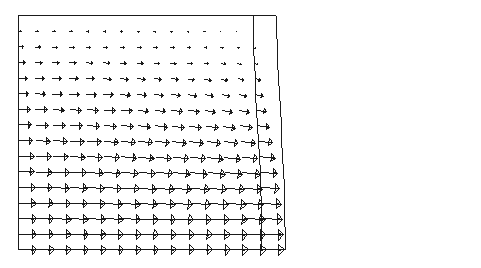
\includegraphics[width=0.45\textwidth]{fill2.png}
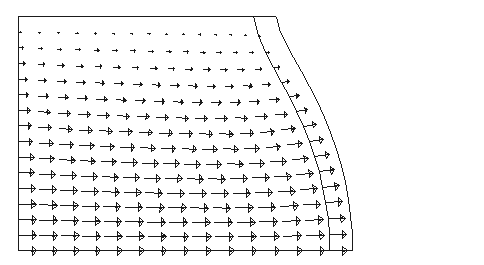
\includegraphics[width=0.45\textwidth]{fill20.png}
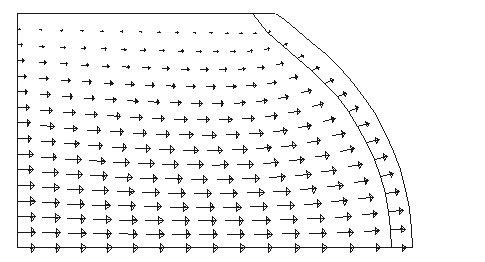
\includegraphics[width=0.45\textwidth]{fill40.png}
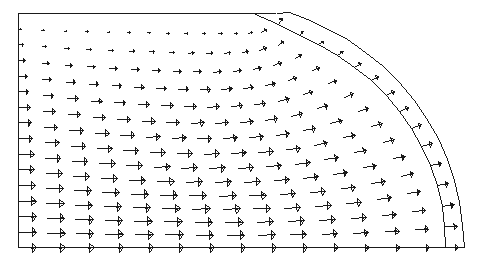
\includegraphics[width=0.45\textwidth]{fill60.png}
\end{center}
\caption{Snapshots of an elastic square being gradually filled by incompressible fluid.}
\end{figure}

\begin{figure}[tbhp]
\begin{center}
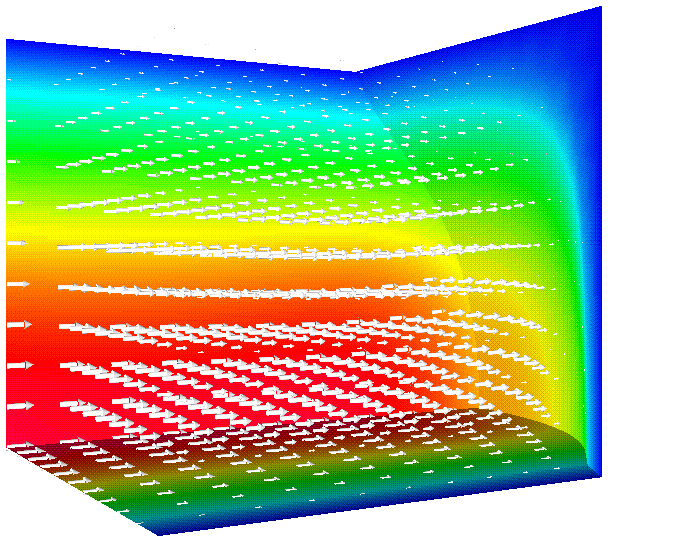
\includegraphics[width=0.45\textwidth]{box3d20.png}
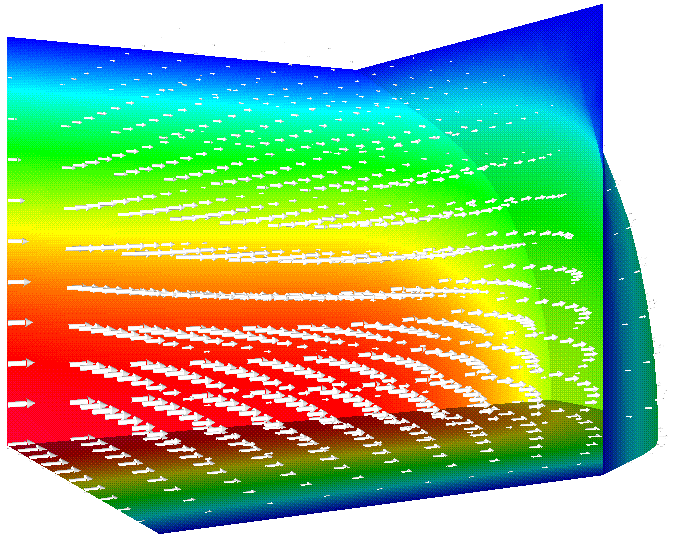
\includegraphics[width=0.45\textwidth]{box3d39.png}
\caption{Snapshots of an elastic cube being gradually filled by incompressible fluid.}
\end{center}
\end{figure}


\bibliography{elmerbib}
\bibliographystyle{plain}
\end{versiona}


\graphicspath{{./}{blockpreconditioning/}}
\chapter{Block preconditioning of Stokes equation}
\noindent
\modinfo{Module name}{Stokes}
\modinfo{Module subroutines}{StokesSolver}
\begin{versiona}
\modinfo{Module authors}{Mika Malinen}
\modinfo{Document authors}{Mika Malinen}
\modinfo{Document edited}{Feb 20th 2006}

\section{Introduction}

The discretization of flow equations leads usually to large linear systems. Since
the direct solution of large linear systems is often too expensive in computation time 
and computer memory requirements, such linear systems are customarily solved
with iterative algorithms, in combination with preconditioning.
%For a discussion of key ideas underlying the preconditioned solution methods
%see, for example, \cite{ESW05}.

The general preconditioning strategy used in Elmer is based on the computation of 
incomplete factorizations. The performance of these preconditioners 
is case-dependent and may
not always be satisfactory. More efficient solution algorithms for a particular
problem can often be developed by exploiting the block structure of the 
linear system. This strategy has been used to develop an alternative
solution method for the linear systems which result from the discretization
of the Stokes equations. In the following a description of this solution 
method will be given.

It should be noted that in Elmer the Stokes equations can be solved with the solver 
for the Navier-Stokes equations. The alternative
solution method described here can however be applied only in connection with 
a special solver for the Stokes equations. This special solver is still
under development and a lot of additional features accessible through 
the Navier-Stokes solver are not available currently.       
Suggestions concerning the further development of this special solver are welcome.   


\section{Theory}

The solver described here can be used to solve numerically the  
Stokes equations.
%accompanied by suitable mixed boundary conditions.
In the evolutionary case the field equations are given by
\begin{equation}\label{stokes_system}
\begin{split}
\rho\frac{\partial\vec u}{\partial t} - \mu \Delta\vec u +\nabla p &= \vec b, \\
\nabla \cdot \vec u &= 0.
\end{split}
\end{equation}
The velocity boundary conditions of Dirichlet type or
homogeneous natural boundary conditions can be imposed on the boundary.
It is noted that
the uniqueness of the pressure solution is assumed to be 
ensured by imposing the normal natural boundary condition        
\begin{equation}\label{Neumann-outflow}
-p + \mu (\nabla\vec u)\vec n\cdot\vec n = 0
%\frac{\partial\vec u}{\partial n} = 0
\end{equation}
on a nontrivial part of the boundary. 

When a boundary can be represented as a coordinate plane,
slip boundary conditions may also given. In the case of slip
boundary condition it is assumed that the normal velocity is prescribed
to vanish ($u_n = \vec u \cdot \vec n = 0$) and the tangential
surface force $s_s$ is related to the tangential velocity $u_s$ by
\begin{equation}\label{slipbc}
s_s = \mu \frac{\partial u_s}{\partial n} = -C_n u_s.
\end{equation}
Here the subscript $s$ refers to the tangential direction and 
$C_n$ is the slip coefficient for the boundary (the subscript $n$ refers to
the normal direction).

If the alternative solution strategy is applied,  
the finite element discretization of (\ref{stokes_system}) is assumed to be 
based on the lowest equal order approximation for the velocity and pressure. 
Such discretization of (\ref{stokes_system}) leads to a linear system 
\begin{equation}\label{discrete-stokes-system}
Ky=b
\end{equation}
where $K$ has the block-structure
\begin{equation}\label{block-structure}
K=\left( \begin{array}{cc} A    & B^T \\
                         B    & C   \end{array}\right). 
\end{equation}
Here $A$ is the coefficient matrix which results from the discretization 
of $-\mu\Delta \vec u$ or the spatial and backward Euler time discretization of
$\rho(\partial\vec u /\partial t) -\mu\Delta \vec u$.
In addition, $C$ is a stabilization matrix
which results from adding a stabilization operator suggested in \cite{Do04}.
%in the case of the lowest equal order approximation.

The iterative solution methods considered here are based on applying a
Krylov subspace method to (\ref{discrete-stokes-system}) 
in combination with a block-preconditioner
\begin{equation}
P= \left( \begin{array}{cc} P_A           & B^T \\
                         0    & P_S   \end{array}\right)  
\end{equation}
where $P_A$ and $P_S$ 
approximate $A$ and the Schur complement of $A$ in $K$.  
In practice, the application of the preconditioner requires that the actions of the inverses 
$P_A^{-1}$ and $P_S^{-1}$ are approximated. 
These tasks can often be done efficiently by applying iterative methods to systems
of type $P_Az_A=r_A$ and $P_Sz_S=r_S$.

The action of the inverse of $P_S$ is constructed in such a way that one has 
in the stationary case \cite{Si94} 
\begin{equation}\label{stationaryPs}
P_S^{-1}r_S \approx -(\frac{1}{\mu}M)^{-1}r_S   
\end{equation}
and in the evolutionary case \cite{Ca88}
\begin{equation}\label{evolutionaryPs}
P_S^{-1}r_S \approx (\frac{\delta t}{\rho}D)^{-1}r_S - (\frac{1}{\mu}M)^{-1}r_S    
\end{equation}
where $r_S$ is a vector in the pressure space, $\delta t$ is the size of time step, and 
$M$ and $D$ are finite element approximations of the identity 
and Laplace operators. It is noted that the Laplace operator in (\ref{evolutionaryPs})
is associated with the homogeneous Dirichlet boundary condition on the part of the boundary
where the boundary condition (\ref{Neumann-outflow}) is given,
while the homogeneous Neumann boundary condition is used on the remaining part
of the boundary.

It is noted that 
the actions of the approximate inverses of the scaled pressure mass matrices in 
(\ref{stationaryPs}) and (\ref{evolutionaryPs}) are always computed 
with the BICGSTAB method. The user can choose a method for 
approximating the action of the inverse of the pressure Laplacian operator in (\ref{evolutionaryPs}).
Several options such as applying an algebraic multigrid V-cycle are available for this computation. 

In the stationary case each action of the preconditioner
depends upon an approximate solution of a Poisson equation for each of the velocity components.
The user can choose a method for this computation.  
In the evolutionary case the action of the inverse of $P_A$ 
is always computed with the BICGSTAB method. 

The outer iterative method which is applied to (\ref{discrete-stokes-system})
is based on either BICGSTAB method or a nested GCR algorithm.
The nested GCR algorithm is based on the idea of solving the new search direction
of the outer GCR iteration from the residual equation which characterizes the 
error in the current approximate solution. The residual equation is solved 
approximately by taking at most $m$ steps of the block-preconditioned GCR algorithm
where $m$ can be controlled by the user.

It is mentioned that 
the method based on BICGSTAB has the benefit of requiring only a small, fixed amount 
of computer memory. A drawback is that the performance may deteriorate when
more inaccurate solutions of preconditioning systems are allowed. 
The nested GCR algorithm has been found to perform robustly with respect to 
inaccuracies in preconditioning, but as compared with BICGSTAB more solution
vectors may need to be saved during the iteration.  


 
  
  
 


\section{Keywords}
\end{versiona}

\sifbegin
\sifitemnt{Material}{material-id}
\sifbegin
\sifitem{Density}{Real} 
This keyword is used to define the density $\rho$.

\sifitem{Viscosity}{Real} 
This keyword is used to define the viscosity $\mu$.

\sifend
\sifend


\sifbegin
\sifitemnt{Solver}{solver-id}
\sifbegin

\sifitem{Equation}{String}
This keyword declares the name of the equation.

\sifitem{Procedure}{File ''Stokes'' ''StokesSolver''}
The name of the file and procedure.

\sifitem{Variable}{String ''Stokes''}
This keyword declares the name of the solution.

\sifitem{Variable Dofs}{Integer}
The value of this keyword defines the number of unknown scalar fields
and must hence equal to $d+1$ where $d$ is the spatial 
dimensionality of the computational domain.
It is noted that the unknown scalar fields are always numbered in such a
way that the highest running number is associated with the pressure
solution. 

\sifitem{Stabilize}{Logical}
By default this keyword is given the value {\tt ''True''} so that
the equal order approximation for the velocity and pressure may be used.

\sifitem{Block Preconditioning}{Logical} 
If the block preconditioning is used, the value of this keyword must 
be {\tt ''True''}. 

\sifitem{Outer Iteration Method}{String}
This keyword is used to define the outer iterative method.
The default method is the nested GCR algorithm. 
In order to use the method based on BICGSTAB the value {\tt ''BICGSTAB''} should be given
for this keyword.  

\sifitem{Max Outer Iterations}{Integer}
When the outer iterative method is based on BICGSTAB,
the value of this keyword defines the maximum number of outer iterations allowed,
i.e. the maximum number of the block preconditioned  
iterations. When the outer iterative method is 
the nested GCR algorithm, this keyword is used to
control restarting so that the outer GCR algorithm is restarted
after each $m$ iteration steps where $m$ is the value of this keyword.

\sifitem{Max Outer GCR Cycles}{Integer}
When the outer iterative method is
the nested GCR algorithm, the value of this keyword defines the maximum number
of restarts allowed in the outer GCR iteration. 
The default value is the unity which corresponds to allowing only one
GCR cycle.

\sifitem{Use Truncation}{Logical}
When the outer iterative method is the nested GCR algorithm,
a truncation strategy may be used in combination with restarting.
If the value {\tt ''True''} is given for this keyword, after restarting
the orthogonalization of the new search direction vector is done
with respect to $m$ previously used search direction vectors where
$m$ is the value of {\tt Max Outer Iterations}
keyword.

\sifitem{Max Inner GCR Iterations}{Integer}
When the outer iterative method is the nested GCR algorithm, 
the value of this keyword defines the maximum number
of inner GCR iterations (it is noted that restarting cannot be used 
in connection with inner GCR iterations)

\sifitem{Linear System Convergence Tolerance}{Real}
When the block preconditioning is used, the value of this keyword defines
the convergence tolerance used in connection with the solution of preconditioning systems.
Ideally, one should try to use a rather large value so that
the cost of preconditioning is not excessive.  

\sifitem{Linear System Max Iterations}{Integer}
When the block preconditioning is used, this keyword is used to define
the maximum number of iterations allowed in the solution of
preconditioning systems of type $P_Az_A=r_A$ and $P_Sz_S=r_S$.

\sifitem{Ratio of Convergence Tolerances}{Real}
This keyword is used to define the convergence tolerance $TOL$ for 
outer iterations. The value of this keyword defines the ratio of   
TOL to the convergence tolerance used in connection with the solution of 
preconditioning systems. Here the convergence tolerance for 
the solution of preconditioning systems is defined
using the {\tt Linear System Convergence Tolerance} keyword. 

\sifitem{Residual Reduction Ratio}{Real}
When the outer iterative method is the nested GCR algorithm,
this keyword may be used to define a stopping criterion 
for the inner GCR iterations (cf.\ the use of 
{\tt Max Inner GCR Iterations} keyword).
The inner GCR iteration is stopped when the new search vector so obtained
is guaranteed to
reduce the norm of the outer iteration residual by a ratio $\epsilon$ where
$\epsilon$ is the value of this keyword.
The default value of this keyword is 0.1.


\sifitem{ILU Order for Schur Complement}{Integer}
In the stationary case the value of this keyword defines 
the fill level for the incomplete LU factorization preconditioner that 
is used in the iterative solution of the linear systems   
involving $P_S$. In the evolutionary case this keyword may be used to
define an incomplete factorization preconditioner for the pressure mass 
matrix $M$ in (\ref{evolutionaryPs}). It should be noted that
in the evolutionary case the usual linear
solver keywords can be used to define an iterative method for the solution of
the pressure Laplacian system in (\ref{evolutionaryPs}). 
It is also noted that if 
the value of this keyword is not given, then
the Jacobi preconditioning will be used instead of incomplete 
factorization preconditioning.

\sifitem{ILU Order for Velocities}{Integer}
In the evolutionary case this keyword may be used to
define an incomplete factorization preconditioner which is 
used in conjuction with the approximation of the action of $P_A^{-1}$.
If the value of this keyword is not given, then
the Jacobi preconditioning will be used instead of incomplete 
factorization preconditioning.
It should be noted that
in the stationary case the usual linear
solver keywords can be used to define an iterative method for the solution of
the systems involving $P_A$.



\sifend
\sifend


\sifbegin
\sifitemnt{Body Force}{bf-id}
\sifbegin

\sifitem{Body Force i}{Real}
This keyword is used to define the i's component of the body force vector $\vec b$.

\sifend
\sifend




\sifbegin
\sifitemnt{Boundary Condition}{bc-id}
\sifbegin

\sifitem{Outflow boundary}{Logical}
If the value {\tt ''True''} is given
for this keyword, then the outflow boundary condition (\ref{Neumann-outflow}) 
will be used.

\sifitem{Slip Boundary}{Logical}
If the slip boundary condition is defined, then the value {\tt ''True''}
must be given for this keyword.

\sifitem{Slip Coefficient i}{Real}
The value of the slip coefficient in (\ref{slipbc}).
Here $i$ refers to the coordinate direction which is parallel to the normal 
direction of the boundary.




\sifend
\sifend

\begin{versiona}
\begin{figure}[h]
  \vspace{-3cm}
  \begin{center}
    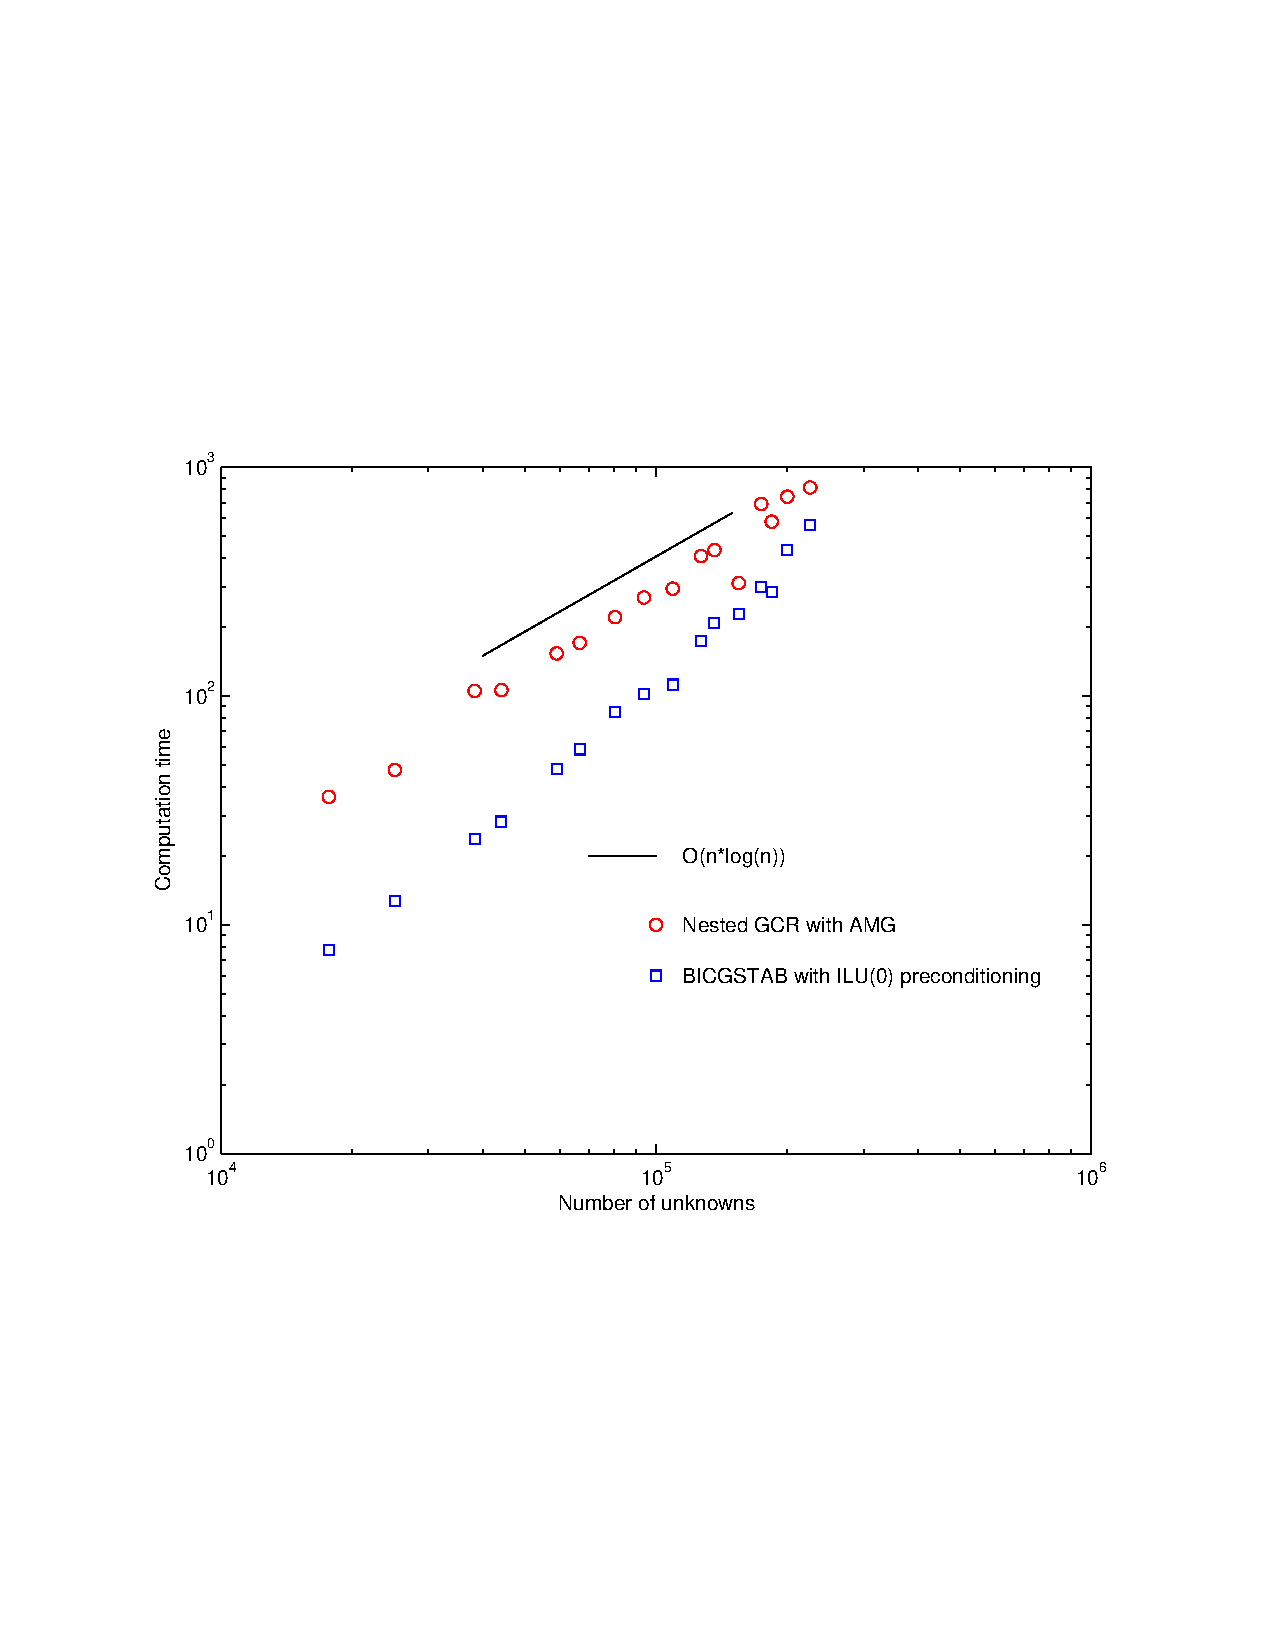
\includegraphics[width=0.49\textwidth]{comptime.pdf}
    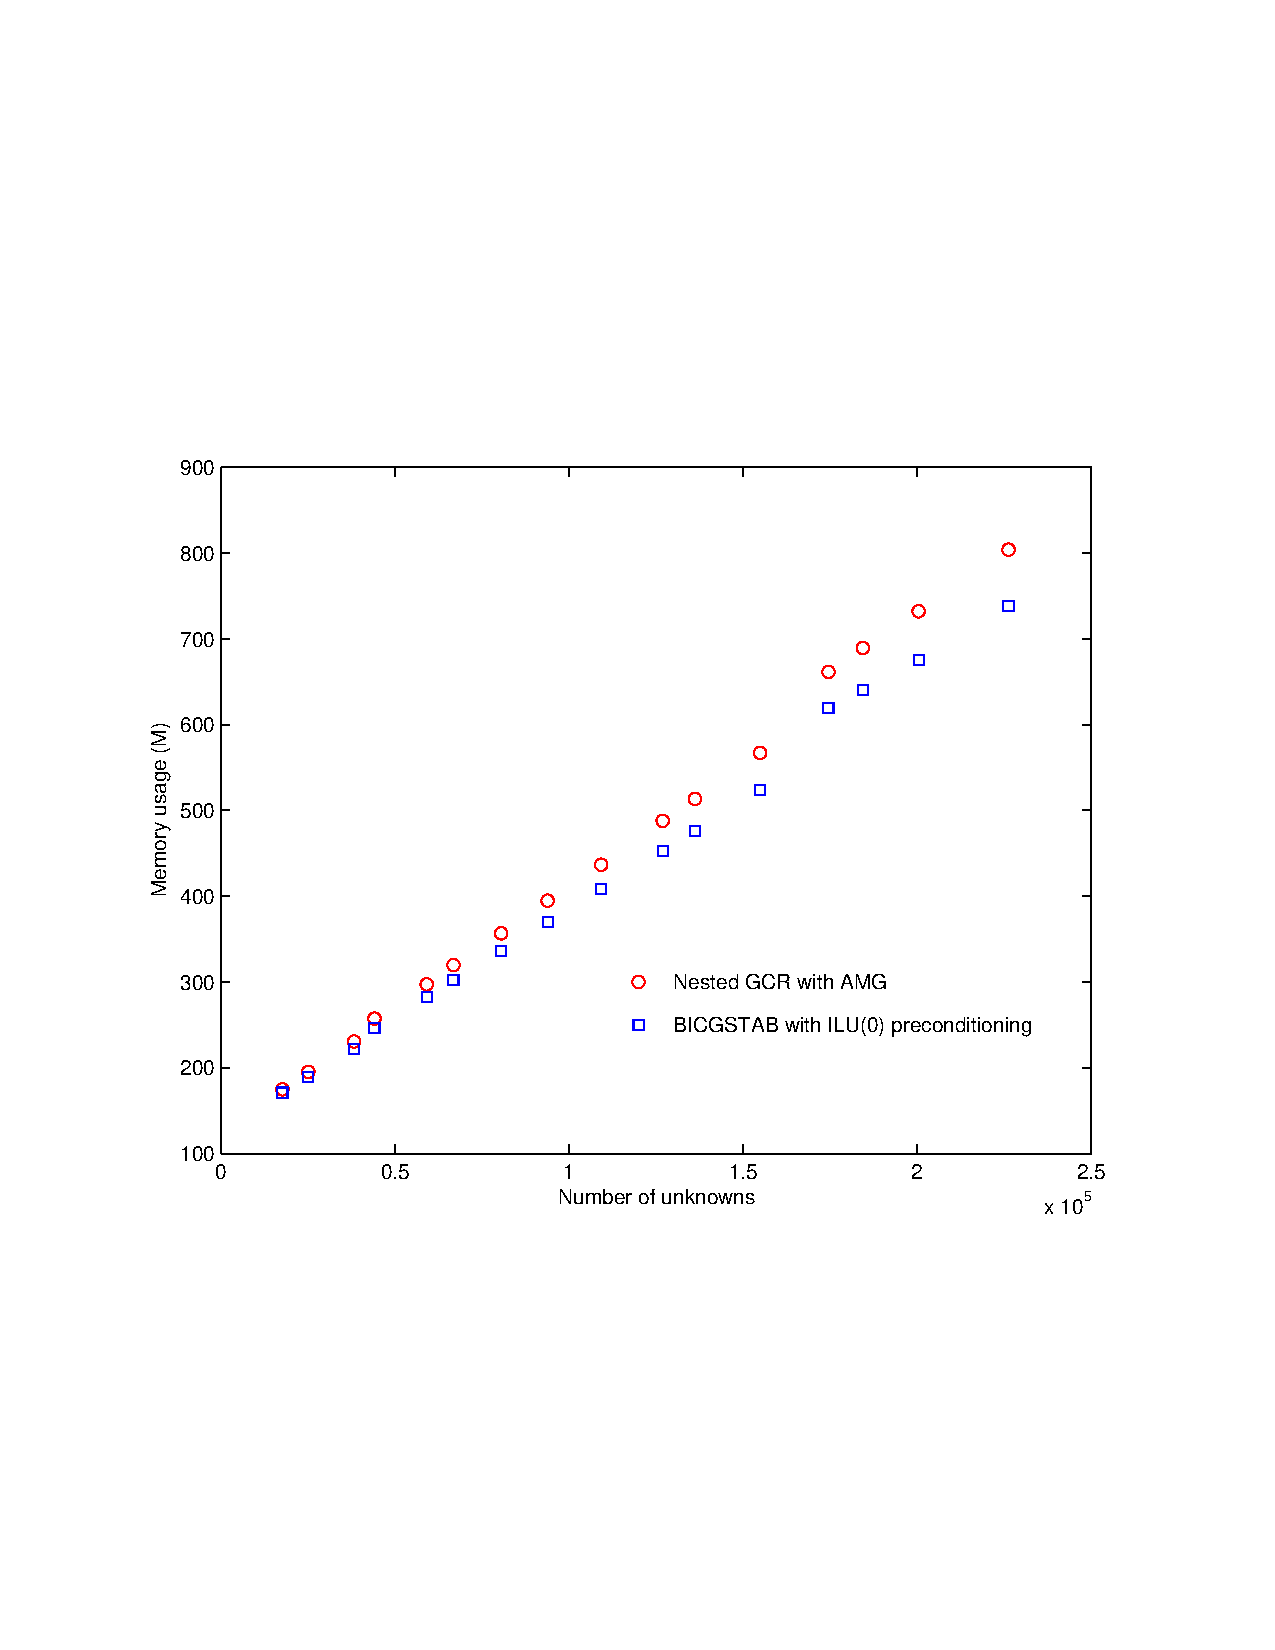
\includegraphics[width=0.49\textwidth]{memory.pdf}
   \end{center}
  \vspace{-3cm}
\caption{A comparison of the nested GCR algorithm with the ILU(0) preconditioned
BICGSTAB method in the case of a three-dimensional test problem. 
In the nested GCR algorithm the algebraic multigrid (AMG) solver was used to 
compute the action of $P_A^{-1}$.}
\end{figure}


\bibliography{elmerbib}
\bibliographystyle{plain}
\end{versiona}


\graphicspath{{./}{operatorsplitting/}}
\Chapter{Operator Splitting Ability}
\noindent
\modinfo{Module name}{TransportEquation, RateOfChange}
\modinfo{Module subroutines}{TransportEquationSolver, RateOfChangeSolver}
\begin{versiona}
\modinfo{Module authors}{Mika Malinen}
\modinfo{Document authors}{Mika Malinen}
\modinfo{Document edited}{Oct 30th 2002}

\section{Introduction}

The drawback of the stabilized finite element formulations available
in Elmer to solve the convection-diffusion equation and Navier-Stokes 
equations is that these methods are computationally expensive, in particular
when the residual-free-bubbles formulation is used.
In evolutionary problems the reduction of computational cost may be attempted 
by applying operator splitting techniques in which the original equation at 
each time step is splitted up into subproblems that are 
easier to solve numerically. The operator splitting technique described in 
the following can be applied to cases in which convection (or advection) 
phenomena are present on account of incompressible fluid flow. 

The key feature of the method described below is that the convective transport 
problem that arises as a subproblem from operator splitting is solved 
numerically by discretizating an equivalent wave-like equation formulation of 
the transport problem. The benefit of this approach is that the wave-like 
equation can be solved without using stabilized finite element formulations.

\section{Theory}

\subsection{Time discretization and operator splitting}

To describe the most essential ideas of operator splitting, consider the 
problem of solving scalar field $T$ such that
\begin{equation}\label{modeleq}
\frac{\partial T}{\partial t}+(A+B)T=f, \quad T=T_0 \ \mathrm{at}\ t=0,
\end{equation} 
where the operators $A$ and $B$ are linear and independent of the time $t$ and 
where the fields $f$ and $T_0$ are given. 

Assume now that the discretization of the time interval on which the solution 
of (\ref{modeleq}) is sought is given. Then,
instead of directly solving the equation (\ref{modeleq}) one 
may attempt the solution of this equation by decoupling the effects of $A$ and 
$B$ at each time step. To be more precise, let $\Delta t$ be the length of the
time interval $[t^n,t^{n+1}]$ and introduce the abbreviations 
$t^{n+\alpha}=t^n + \alpha\Delta t$ and $T^{n+\alpha}=T(t^{n+\alpha})$. 
Given $T^n$ the following operator splitting scheme may be used to solve
an approximation to $T^{n+1}$:    
\begin{equation}\label{os-scheme}
\begin{split}
\frac{\partial T}{\partial t}+A T &= f,\quad \mathrm{on}\ (t^n,t^{n+1/2}),
\quad T(t^n)=T^n, \quad T^{n+1/2}=T(t^{n+1/2}), \\
\frac{\partial T}{\partial t}+B T &= 0,\quad \mathrm{on}\ (0,\Delta t),
\quad T(0)=T^{n+1/2}, \quad \hat{T}^{n+1/2}=T(\Delta t),  \\ 
\frac{\partial T}{\partial t}+A T &= f,\quad \mathrm{on}\ (t^{n+1/2},t^{n+1}),
\quad T(t^{n+1/2})=\hat{T}^{n+1/2},\\
T^{n+1}&=T(t^{n+1}).
\end{split}
\end{equation}
The scheme (\ref{os-scheme}) can be adapted to the solution of the heat 
equation as well as Navier-Stokes equations. In both cases $B$ is taken
to be the convection operator $\vec u \cdot \nabla$ where $\vec u$  
is the velocity field satisfying the incompressibility constraint, while
the interpretation of $A$ is case-dependent. 

In the case of the heat equation  
\begin{equation}
\begin{split}
&\frac{\partial T}{\partial t}+(\vec u\cdot\nabla) T-\nabla\cdot(k\nabla T) = 
f \quad \mathrm{in}\ \Omega \times (0,t_N), \\
&T = g  \ \mathrm{on}\ \Gamma_D, \quad  
-k\nabla T \cdot \vec n = q \ \mathrm{on}\ \Gamma_N, \\  
&T = T_0 \ \mathrm{at}\ t=0, 
\end{split}
\end{equation}
with $\vec n$ being the outward unit normal vector at the boundary 
$\partial\Omega=\Gamma_D \cup \Gamma_N$, the application of the operator 
splitting scheme introduced above yields the system 
\begin{equation}
\begin{split}
&\frac{\partial T}{\partial t}-\nabla\cdot(k\nabla T) = f \quad \mathrm{in}\ 
\Omega\times(t^n,t^{n+1/2}), \\
&T=g \ \mathrm{on}\ \Gamma_D, \quad
-k\nabla T \cdot \vec n = q \ \mathrm{on}\ \Gamma_N, \quad T(t^n)=T^n, \\ 
&T^{n+1/2}=T(t^{n+1/2}),
\end{split}
\end{equation}
\begin{equation}\label{transportequation}
\begin{split}
&\frac{\partial T}{\partial t}+(\vec u\cdot\nabla) T = 0 \quad \mathrm{in}\ 
\Omega \times (0,\Delta t), \\ 
&T=g \ \mathrm{on}\ \Gamma_D \cap \Gamma^-, \quad T(0)=T^{n+1/2} \\
&\hat{T}^{n+1/2}=T(\Delta t),
\end{split}
\end{equation}
\begin{equation}
\begin{split}
&\frac{\partial T}{\partial t}-\nabla\cdot(k\nabla T) = f \quad \mathrm{in}\ 
\Omega\times(t^{n+1/2},t^{n+1}), \\ 
&T=g \ \mathrm{on}\ \Gamma_D, \quad 
-k\nabla T \cdot \vec n = q \ \mathrm{on}\ \Gamma_N, \quad
T(t^{n+1/2})=\hat{T}^{n+1/2},\\
&T^{n+1}=T(t^{n+1}),
\end{split}
\end{equation}
where $\Gamma^-$ is the inflow boundary defined by $\Gamma^- = \{ x\ \vert\ 
x \in \partial\Omega,\ \vec u(x)\cdot \vec n(x) < 0 \}$.

One is thus lead to solve two time-dependent Poisson 
equations and the convective transport problem (\ref{transportequation})
at each time step.
One may expect that the error inherent from the operator splitting with 
respect to time is of $O(\Delta t^3)$, so in the solution of
the three subproblems it is reasonable to use time discretization schemes that
retain second order accuracy.
While the Poisson equation can be solved efficiently by using standard FE 
techniques, the convective transport problem requires specific treatment.  
This equation may be solved numerically without using a stabilized finite 
element formulation by discretizating an equivalent wave-like equation
formulation. This method is described in Section~\ref{Waveequationsection}.

The operator splitting scheme (\ref{os-scheme}) can also be adapted to the 
solution of the Navier-Stokes equations by separating incompressibility and 
diffusion from convection.
In the case of constant kinematical viscosity and Dirichlet type boundary 
conditions over the entire boundary one obtains the system \cite{DG97}  
\begin{equation}
\begin{split}
&\frac{\partial \vec u}{\partial t}-\nu\Delta\vec u+\nabla p = \vec f \quad 
\mathrm{and} \quad \nabla\cdot\vec u \quad
\mathrm{in}\ \Omega\times(t^n,t^{n+1/2}), \\ 
&\vec u = \vec g \quad \mathrm{on}\quad \partial\Omega, \\ 
&\vec u(t^n)=\vec u^n, \quad \vec u^{n+1/2}=\vec u(t^{n+1/2}), 
\end{split}
\end{equation}
\begin{equation}\label{NS-transportequation}
\begin{split}
&\frac{\partial \vec u}{\partial t}+(\vec u^{n+1/2}\cdot\nabla)\vec u=\vec 0 
\quad \mathrm{in}\ \Omega \times (0,\Delta t) \ \mathrm{and} \ \vec u=\vec g \ 
\mathrm{on}\ \Gamma^-,  \\ 
&\quad \vec u(0)=\vec u^{n+1/2}, \quad \vec{v}^{n+1/2}=\vec u(\Delta t),
\end{split}
\end{equation}
\begin{equation}
\begin{split}
&\frac{\partial \vec u}{\partial t}-\nu\Delta\vec u+\nabla p = \vec f \quad 
\mathrm{and} \quad \nabla\cdot\vec u \quad
\mathrm{in}\ \Omega\times(t^{n+1/2},t^{n+1}), \\ 
&\vec u = \vec g \quad \mathrm{on}\quad \partial\Omega, \\ 
&\vec u(t^{n+1/2})=\vec{v}^{n+1/2}, \quad \vec u(t^{n+1})=\vec u(t^{n+1}), 
\end{split}
\end{equation}
In this case one is lead to solve two time-dependent Stokes equations and
the convective transport problem (\ref{NS-transportequation}), which, when
written component-wise, consists 
of independent scalar equations of the same type as in 
(\ref{transportequation}).
  

\subsection{Wave equation approach to the convective transport problem}
\label{Waveequationsection}

If the velocity vector $\vec u$ does not depend on the time $t$ and satisfies 
the incompressibility constraint $\nabla\cdot\vec u=0$, the equation 
(\ref{transportequation}) can be written equivalently as (cf.\ \cite{Wu97})
\begin{equation}
\begin{split}
\frac{\partial^2 T}{\partial t^2}-\nabla \cdot \left( \vec u(\vec u \cdot 
\nabla T) \right)=0 \quad  \mathrm{in}\ \Omega \times (0,\Delta t), \\
T=T^{n+1/2}\quad \mathrm{and}\quad 
\frac{\partial T}{\partial t}= -\vec u \cdot \nabla T\quad \mathrm{at}\ t=0 \\
\quad T=g \ \mathrm{on}\ \Gamma_D \cap \Gamma^-, \quad 
\frac{\partial T}{\partial t}= -\vec u \cdot \nabla T \quad \mathrm{on}\ 
\partial\Omega \backslash \Gamma^-. \\
\end{split}
\end{equation}
This wave-like equation can be solved using standard FE techniques.


\section{Limitations}

Some limitations result from the current implementation:
\begin{itemize}
\item Rectangular Cartesian coordinate system is assumed.

\item Although the velocity field in the convection operator can be taken to 
be the velocity solution to the Navier-Stokes equations, it is presumed, 
however, that the inflow boundary for the velocity field is known a priori
(this knowledge is needed so as to impose boundary conditions).
 
\item Each of the three time-dependent subproblems corresponding to the scheme 
(\ref{os-scheme}) is solved taking only one time step. 
The wave-like equation formulation of the convective transport problem
is discretizated in time using the 
trapezoidal rule (also known as the Crank-Nicolson method). The user can
control only the time discretization scheme that is used in the solution of
the Poisson or Stokes equation corresponding to the operator $B$ 
(keyword {\tt Timestepping Method} in Simulation section).  

\item The number of time steps should be even since the user is required to
specify the points $t^n$ as well as $t^{n+1/2}$. The results written to
the result file after odd time steps represent the solution after pure 
convection step. Physically meaningful results satisfying all essential 
boundary conditions may be written to the result file after even time steps.  


\end{itemize}

\section{Examples}

The reader is referred to Elmer Tutorials for illustrative examples 
showing also how to write Elmer Solver input data.  

\end{sectiona}

\section{Keywords}
The following keywords are particularly related to operator splitting 
ability.
\sifbegin
\sifitemnt{Simulation}{}
\sifbegin
\sifitem{Simulation Type}{String} 
The simulation type must be set to be {\tt Transient}. 
\sifitem{Coordinate System}{String} 
The coordinate system must be set to be one of the following options:
{\tt Cartesian 1D, Cartesian 2D }\  or\ \ {\tt Cartesian 3D}.
\sifend

\sifitemnt{Equation}{eq-id} 

Equation section is used to declare the set of equations obtained by operator 
splitting. To include the convective transport problem in the set of the
equations to be solved the following two declarations are needed: 
%To solve the wave-like equation formulation of the convective
%transport problem the following two declarations are needed:  
\sifbegin
\sifitem{Transport Equation}{Logical} 
When the value of this keyword is set to be {\tt True}, the wave-like equation 
formulation of the convective transport problem is solved.    
\sifitem{Rate of Change Equation}{Logical}
Setting the value of this keyword to be {\tt True} enables the solution of 
the Galerkin approximation to the rate of change of the field subject 
to the convection operator at the beginning of pure convection step. This 
approximate field is used as initial condition in the solution of the 
convective transport problem. 
\sifend


\sifitemnt{Solver}{solver-id}

The following keywords should be included in Solver section that contains
solver parameters for {\tt Rate Of Change Equation}, i.e.\ in that  
section that has the declaration \\ \\
{\tt Equation String "Rate of Change Equation".}

\sifbegin
\sifitem{Procedure}{File "RateOfChange"\ "RateOfChangeSolver"} 
The name of the file and subroutine.

\sifitem{Advection Variable}{String}
This keyword is used to declare the quantity which is subject to the convection
operator.

\sifitem{Variable}{String "Udot0"}
The name {\tt Udot0} is used for the rate of change of the field 
subject to the convection operator at the beginning of pure convection step.  

\sifitem{Variable Dofs}{Integer}
The value of this keyword should equal to the dimension of the vector field 
subject to the convection operator.
 
\sifitem{Advection}{String}
This keyword defines the type of the velocity field in the convection operator
and may be set to be either {\tt Constant} or {\tt Computed}. 
If set to be {\tt Computed}, the velocity field in the convection 
operator is taken to be the velocity solution to the Navier-Stokes equations.
\sifend


The following keywords should be included in Solver section that contains
solver parameters for {\tt Transport Equation}, i.e.\ in that  
section that has the declaration \\ \\
{\tt Equation String "Transport Equation".}

\sifbegin
\sifitem{Procedure}{File "TransportEquation"\ "TransportEquation\-Solver"} 
The name of the file and subroutine.

\sifitem{Time Derivative Order}{Integer 2}
The wave-like equation is of second order in time.

\sifitem{Advection Variable}{String}
This keyword is used to declare the quantity which is subject to the 
convection operator. 

\sifitem{Variable}{String "U"}
The name {\tt U} is used for the solution of the convective transport problem.
  
\sifitem{Variable Dofs}{Integer}
The value of this keyword should equal to the dimension of the vector field 
subject to the convection operator.

\sifitem{Rate of Change Equation Variable}{String}
The value of this keyword should equal to that of the {\tt Variable} 
keyword in Solver section containing solver parameters for 
{\tt Rate Of Change Equation}.

\sifitem{Advection}{String}
This keyword defines the type of the velocity field in the convection operator
and may be set to be either {\tt Constant} or {\tt Computed}. If set 
to be {\tt Computed}, the velocity field in the convection operator is 
taken to be the velocity solution to the Navier-Stokes equations.
\sifend


\sifitemnt{Material}{material-id}
\sifbegin
\sifitem{Advection Velocity i}{Real} 
If the velocity vector in the convection operator is of constant type, then 
this keyword is used to define the i's component of the velocity vector in the 
convection operator. 
\sifend


\sifitemnt{Boundary Condition}{bc-id}
\sifbegin
\sifitem{Udot0 i}{Real}  
The $i$'s component of {\tt Udot0} should be prescribed on that part of the
inflow boundary where the corresponding component of the quantity subject to 
the convection operator (declared using the keyword {\tt Advection Variable}) 
is prescribed.

\sifitem{U i}{Real} 
The $i$'s component of {\tt U} should be prescribed on that part of
the inflow boundary where the corresponding component of the quantity
subject to the convection operator (declared using the keyword {\tt
Advection Va\-ri\-ab\-le}) is prescribed so that the values of the two
components equal.

\sifend 
\sifend

\bibliography{elmerbib}
\bibliographystyle{plain}



\graphicspath{{./}{streamlines/}}
\chapter{\Idx{Streamlines}}
\noindent
\modinfo{Module name}{\Idx{StreamSolver}}
\modinfo{Module subroutines}{StreamSolver}
\begin{versiona}
\modinfo{Module authors}{Mika Juntunen}
\modinfo{Document authors}{Mika Juntunen}
\modinfo{Document edited}{July 30th 2003}

\section{Introduction}

Streamline is a line in flow whose tangent is parallel to velocity field
$\vec u$ of the flow in every point $\vec x$. It should be noted that the path of 
material is generally not the same as streamlines. There is also third set
of closely related lines, namely streak lines. On certain streak line
lie all those flow elements that at some earlier instant passed through
certain point in domain. Of course, the streak lines are generally different
than streamlines but when the flow is steady all three set of lines coincide.

Streamlines are mainly used in providing a picture of the flow field. 
Drawing streamlines so that neighbouring streamlines differ by the same amount, 
gives a picture where direction and magnitude change of flow are clearly prescribed.

\section{Theory}

We are restricted here to the incompressible, steady flow in 2D geometry.
The geometry may be 3D, but it must effectively be 2D as in axis symmetric
geometry.

In 2D cartesian geometry stream function $\psi$ is defined
\begin{equation}\label{e:def2d}
u \, = \, \frac{\partial \psi}{\partial y} \, , \quad
v \, = \, - \frac{\partial \psi}{\partial x} \,.
\end{equation}
Here the geometry is $(x,y)$ and the corresponding flow is $\vec u = (u,v)$.
Let $\Omega$ be the domain of the flow and $\vec v$ a test function for the flow.
Definition~\eqref{e:def2d} leads to finite element approximation
\begin{equation}\label{e:fem2D}
\int_\Omega \nabla \psi \cdot \vec v \, \text{d}\Omega
=
\int_\Omega \vec u^\perp \cdot \vec v \, \text{d}\Omega
\end{equation}

In axis symmetric geometry the mass conservation calculated in a diffenrent way.
This leads to following definition for stream function. 
\begin{equation}\label{e:def_axis}
u \, = \, \frac{1}{r}\frac{\partial \psi}{\partial r} \, , \quad
v \, = \, - \frac{1}{r}\frac{\partial \psi}{\partial z} \,
\end{equation}
where the cylinderical coordinates are $(z,r,\phi)$, velocity components
are $(u,v,w)$ and axis of symmetry is $z$ i.e. $r=0$.
This function is sometimes called the \emph{\Idx{Stokes stream function}} 
and it is not as informative as the stream function in cartesian case.
Of course the finite element approximation is a bit different.
\begin{equation}
\int_\Omega \nabla \psi \cdot \vec v \, \text{d}\Omega
=
\int_\Omega \vec u^\perp \cdot \vec v r \, \text{d}\Omega
\end{equation}
Here the $\phi$ component of the flow is excluded.

From definitions~\eqref{e:def2d} and~\eqref{e:def_axis} it is apparent that 
stream function is constant along the streamlines. So drawing the contours 
of stream function gives the streamlines.

\section{Limitations}

Some limitations of the current implementation:
\begin{itemize}

\item The flow field is asumed to be incompressible.

\item There is no dependency on time. Solver can be used in transient cases, but
it only produces the streamlines of the current flow field as if it was steady. 

\item Only 2D cartesian and axis symetric coordinate systems are implemented.

\item Solver gets the velocity field from user defined variable. In cartesian case
it assumes that first degree of freedom is the $x$-component and the second is the
$y$-component of the velocity. In axis symmetric case it assumes that the first
degree of freedom is the $r$-component and the second is the $z$-component of
the velocity field.

\item User can define the node whose value is first set to zero. This \emph{shouldn't}
have affect on results if the normal stream function is used in cartesian coordinates
and Stokes stream function in axis symmetric coordinates. However, if used stream function
is forced to something else, the position of the first node usually has a large
effect on results. 
This is because the mass conservation is calculated differently.

\end{itemize}


\section{Keywords}
\end{versiona}


\sifbegin
  \sifitemnt{Simulation}{}
  \sifbegin
    \sifitem{Coordinate System}{String} 
    The coordinate system should be set to be one of the following options:
    {\tt Cartesian 2D}~~ or~~ {\tt Axi Symmetric}. 
  \sifend

  \sifitem{Solver}{solver-id} 
  All the keywords beginning {\tt Linear System} can be used. 
  They are explained elsewhere. 
  \sifbegin
    \sifitem{Equation}{String}
    The name you want to give to the solver, for example {\tt StreamSolver}.

    \sifitem{Procedure}{File "StreamSolver"\ "StreamSolver"} 
    The name of the file and subroutine.

    \sifitem{Variable}{String}
    The name you want to call the solution, for example {\tt StreamFunction}.

    \sifitem{Variable Dofs}{Integer 1}
    The degree of freedom of the variable. Stream function is scalar so this must be set to 1.
 
    \sifitem{Stream Function Velocity Variable}{String}
    The name of the velocity field variable. FlowSolvers solution is
    called {\tt Flow Solution} and this is also the default value.

    \sifitem{Stream Function First Node}{Integer}
    Number of the node that is first set to zero. Non-positive values are set to 1 and
    too large values are set to largest possible i.e. 'the last node'. Default is 1.

    \sifitem{Stream Function Shifting}{Logical}
    Shift the smallest value to zero. Default is {\tt True}.

    \sifitem{Stream Function Scaling}{Logical}
    Scale largest absolut value to 1. Default is {\tt False}.

    \sifitem{Stokes Stream Function}{Logical}
    This keyword forces the stream function type regardles of the coordinate system.
    If the coordinate system is axis symmetric, then the default is {\tt True},
    else the default is {\tt False}.
  \sifend
\sifend

%\bibliography{elmerbib}
%\bibliographystyle{plain}




\graphicspath{{./}{linearrestriction/}}
\chapter{\Idx{Linear Constraints}}
\noindent
\modinfo{Module name}{included in solver (SolverUtils)}
\modinfo{Module subroutines}{\Idx{SolveWithLinearRestriction}}
\modinfo{Module authors}{Mika Juntunen}
\modinfo{Document authors}{Mika Juntunen}
\modinfo{Document edited}{August 5th 2003}

\section{Introduction}
This subroutine allows user to solve problems with linear constraints.
Here constraints are forced with \Idx{Lagrange multipliers}. This method,
however, does not always lead to a well-posed problem. Conditions that ensure
a (unique) solution are excluded here, but the conditions are found in many
books (check for example~\cite{c:girault}).  

\section{Theory}
The problem at hand is
\begin{equation}\label{e:problem}
\min_x \, x^T A x - x^T f
\end{equation}
Let's assume that we can solve this. Now we also want that the solution
solves the system $Bx = g$. This gives constraints to our solution.
The rank of $B$ should be less or equal to the rank of $A$.
Loosely speaking, the number of rows in $B$ should be less or equal to the
number of rows in $A$. The method of Lagrange multipliers fixes these two
equations together and gives a new functional to minimize.
\begin{equation}
\min_x \, x^T A x - x^T f +\lambda^T ( Bx-g )
\end{equation}
If $A$ is symmetric, then simple variational approach leads to solving
$x$ out of system
\begin{equation}
\begin{pmatrix}
A & B^T \\
B & 0 
\end{pmatrix} 
\begin{pmatrix}
x \\
\lambda
\end{pmatrix}
=
\begin{pmatrix}
f \\
g
\end{pmatrix}
\end{equation}
Symmetry of $A$ is not always needed, but then more powerful methods have to be used
to get to the above system.

\section{Limitations}
\begin{itemize}
\item \textbf{General usage of the subroutine} \newline
This subroutine can not be used by just adding keywords to solver input file.
You must somehow create the constraint matrix and then call for SolveWithLinearRestriction
in your own subroutine or function. The reader is encouraged to check for details
in ElmerTutorials.

\item \textbf{EMatrix-field} \newline
The EMatrix-field of the solved system matrix is used passing constraint matrix to
SolveWithLinearRestriction. This will be a problem if some other function or subroutine
tries to use the EMatrix-field. EMatrix-field of the constraint-matrix is internally
used by SolveWithLinearRestriction and should therefor be left alone.

\item \textbf{Exported Multipliers} \newline
The length of the vector that holds the multipliers is limited to be a multiply
of the number of nodes in mesh. This means that the vector usually has extra entries.
These entries are set to zero. This leads to problems in extracting the correct 
values from the result file. Also post processing with ElmerPost is at least tricky.

\item Parallel solving is not yet implemented.

\end{itemize}

\section{Keywords}

\sifbegin
  \sifitemnt{Solver}{solver-id}
  \sifbegin
    \sifitem{Export Lagrange Multiplier}{Logical}
    If the multiplier has some physical meaning, you can save it to result file
    and to post file. This feature has certain drawbacks, check subsection Limitations.
    Default is {\tt False}.

    \sifitem{Lagrange Multiplier Name}{String}
    The name you want to call the exported multipliers. This keyword has no meaning if
    the previous keyword is set to {\tt False}. Default name is 
{\tt LagrangeMultiplier}.
  \sifend
\sifend

\bibliography{elmerbib}
\bibliographystyle{plain}




\graphicspath{{./}{arterybc/}}
\chapter{Outlet Boundary Condition for Arterial Flow Simulations}

\modinfo{Module name}{\Idx{ArteryOutlet}}
\modinfo{Module subroutines}{\Idx{OutletCompute}, OutletInit, OutletPres, OutletdX, OutletdY}
\modinfo{Module authors}{Esko J�rvinen, Mikko Lyly, Peter R�back}
\modinfo{Document authors}{Esko J�rvinen}
\modinfo{Document created}{April 28th 2006}
\modinfo{Document edited}{April 28th 2006}

\section{Introduction}

Arterial elasticity is a fundamental
determinant of blood flow dynamics in arteries, such as the 
aorta and its daughter vessel, that face the largest displacements and which 
takes care of the cushioning of the stroke volume.  Simulation of such a 
phenomenon requires simultaneous solving of the equations governing both the 
fluid flow and wall elasticity.  To be able to perform accurate 
fluid-strucrure interaction (FSI) simulations, only a segment of the 
circulatory system can be studied at a time. For these 
artificially truncated segments, which are naturally unbounded domains and 
in interaction with the rest of the circulation domain, one should construct
in the numerical models boundary conditions which do not exhibit any
unphysical behaviour, which operates 
transparently, and are also capable to transport a sufficient amount of 
information over the boundary.  

A natural boundary condition at the outlet of a numerical FSI flow model of an 
artery is not a proper choice because it  does not exhibit enough correct 
physiological behavior of the flow, 
and from the point of view of numerical approximation, 
it causes non-physiological reflections of the wave at the boundary. 
If measured data of both the pressure (or velocity) and the wall 
displacement at the outlet boundary are not available, 
%i.e.~the displacement of the wall can not be predescribed, 
the only way to get the outlet boundary of a higher order, 2D or 3D model 
sufficiently specified is to combine the model
with some lower order model, such as a 1D or lumped model.

In order to get the outlet of the arterial FSI model to behave
transparently in such cases when only forward travelling 
waves are considered, a simple characteristic equation of the
of the one dimensional FSI model can be combined
with the higher order model.

\section{Theory}

The conservation equations for a flow in an elastic artery in one 
dimension may be expressed as

\begin{equation}
\left\{ \begin{array}{ll}
{{\partial A}\over{\partial t}} + {{\partial Q}\over{\partial x}} = 0 & \\
& \\
{{\partial Q}\over{\partial t}} + {{\partial}\over{\partial x}}
({{Q^2} \over {A}}) 
+ {{A} \over {\rho}}{{\partial p}\over{\partial x}}= 0, & \\
%& \\
%p = \beta(\sqrt{A}-\sqrt{A_0}),
        \end{array}
\right. 
\label{eq:1Dyhtalot}
\end{equation}

where $Q$ is the volume flow, $A$ the cross section area of the artery, $p$ is 
the pressure and $x$ is the axial coordinate~\cite{hughes2}.  In order to get the 
system (\ref{eq:1Dyhtalot}) close, an equation relating the area 
$A$ to the pressure $p=p(A)$ is derived applying the theory of thin shell 
structures. Assuming a cylindrical shell, and neglecting the rotation on the 
shell cut plane, and the movements of the structure in the axial 
and circumferential directions, as well as applying the Kirchhoff-Love
assumption, the energy balance equations is reduced to

\begin{equation}
{{E~h^3}\over{12(1-\nu^2)}}~{d_R}^{(4)} + 
{{E~h}\over{(1-\nu^2)}}~{{1}\over{{R_m}^2}}~d_R = p, 
\label{eq:enebala}
\end{equation}

where $R_m$ is the radius to the midplane of the wall, $E$, $\nu$ and $d_R$
are the Youngs modulus, the Poisson ratio and the radial displacement of wall,
respectively.  Assuming that the first term on the left side in the
equation (\ref{eq:enebala}) is much smaller than the second term, we 
can give the pressure-area relation in the form

%\[
\begin{equation} 
p = p_{ext}+\beta(\sqrt{A}-\sqrt{A_0}),
\hspace{10mm} \beta={{\sqrt{\pi}hE}\over{(1 - \nu^2 ) A_0}}.
\label{eq:painebeta}
\end{equation} 
%\]

The pressure is scaled to be equal to external pressure $p_{ext}$ 
with corresponding reference artery cross sections area $A_0$.  
%Hereafter we set $p_{ext}$ equal to zero.

The equations (\ref{eq:1Dyhtalot}) and (\ref{eq:painebeta}) form a closed 
system for the simulations of flow in an elastic tubes.  The equations may be 
written in conservative form which is strictly hyperbolic with two distinct 
real eigenvalues 
$\lambda_{1,2} = \bar{u}\pm c$, where 
$\bar{u}={{Q}/{A}}$ is the average axial velocity, 
$c = \sqrt{({{{A}/{\rho_{f}}}) ({{\partial p}/{\partial A}}})} =  
\sqrt {{\beta \sqrt{A} /(2{\rho_{f}})}} $ is the speed 
of sound, and $\rho_{f}$ is the density of blood. The system %of equations 
%(\ref{eq:konservatiivinen2}) 
can be further decomposed into a set of the equations 
for the characteristic variables $W_i$, which are the components of the vector
$W=T^{-1}U ~({{\partial W}\over{\partial U}}=T^{-1}$)
, $U = [A,Q]^{T} ~\cite{godlewski_raviart}$.  These equations are 

\begin{equation}
{{\partial W_i}\over {\partial t}}+
\lambda_i{{\partial W_i}\over {\partial x}}=0,
\label{eq:W-yhtalot}
\end{equation}

and the characteristic variables are 

\[
%\begin{eqnarray}
W_{1,2}= 
%\bar{u}\pm 4c = 
%\bar{u} \pm 2 \sqrt{ {{2}\over{\rho}} } \sqrt{p + \beta \sqrt{A_0}} =
{{Q}\over{A}}\pm 2\sqrt{{{2}\over{\rho_{f}}} + \beta \sqrt{A}}.
\label{eq:Weet}
%\end{eqnarray}
\]

When considering a pulse propagation in a straight, infinitely long homogeneous
conduit, without any bifurcations or other objects which might cause reflections 
of the pulse, i.e.~any backward travelling waves does not exists, the 
computations can be done using only the first of equations in 
(\ref{eq:W-yhtalot}), i.e.

\[
%\begin{equation}
{{\partial W_1(U)}\over {\partial t}}+
\lambda_1(U){{\partial W_1(U)}\over {\partial x}}=0.
\label{eq:ekaW-yhtalo}
%\end{equation}
\]
 
This equation is solved in this Elmer outlet bondary condition for 
arterial flow simulations solver.
The connection of the one dimensional model to the test models at the 
their outlets is done applying the following coupling~\cite{formaggia1}

\begin{eqnarray*}
\left\{ \begin{array}{ll}
dR^{-}=dR^{+}& \\
\sigma^{-}=p^{+}& \\
W_1 = g_1(A^{-},Q^{-},p^{-}),&
        \end{array}
\right. 
\label{eq:jatkuvuusehdot}
\end{eqnarray*}

where $dR$ and $\sigma$ are radial displacement of the artery wall
and fluid traction, respectively.
The superscript '--' denotes the values in the higher order 
models, and superscript '+' to the values in the 1D model. 




%\hspace{10mm} \beta={{\sqrt{\pi}hE}\over{(1 - \nu^2 ) A_0}}.

\section{Keywords} 

\subsection*{Keywords of FlowSolve}

\sifbegin
\sifitem{Initial Condition}{ic id}
For making the initial guess for the characteristic variable $W_1$
\sifbegin
\sifitem{Wnodal} {Variable Coordinate \\ 
Real Procedure "ArteryOutlet" "OutletInit"}
\sifend
\sifend

\sifbegin
\sifitem{Material}{mat id}
Material properties for the one dimensional section.
\sifbegin
\sifitem{Density}{Real}
Density of blood
\sifitem{Artery Wall Youngs Modulus}{Real}
Young's modulus of the artery
\sifitem{Artery Radius}{Real} 
Radius of the artery to the midplane of the artery wall
\sifitem{Artery Wall Thickness}{Real}
Wall thichness of the artery
\sifitem{Artery Poisson Ratio}{Real}
Poisson ration of the artery
\sifend
\sifend

\sifbegin
\sifitem{Solver}{solver id}
Keywords for the one dimensional solver.
Note that all the keywords related to linear solver (starting
with {\tt Linear System})
may be used in this solver as well.  They are defined elsewhere. 
\sifbegin
\sifitem{Equation}{String [Artery Outlet Solver]}
%\sifitem{Time Derivative Order}{[1]}
%\sifitem{Stabilize}{Logical [False]}
\sifitem{Variable}{[Wnodal]}
The variable which is solved 
\sifitem{Variable DOFs}{[1]}
\sifitem{Procedure}{File "ArteryOutlet" "OutletCompute"}{}
The name of the file and the subroutine
\sifend
\sifend

\sifbegin
\sifitem{Equation}{eq id}
The equation section is used to define a set of equations for a body
or set of bodies 
\sifbegin
\sifitem{Artery Outlet Solver}{Logical [True]}
If set {\tt True}, the solver is used.  The name of the solver must
match with the name in the {\tt Solver} section
\sifend
\sifend

\sifbegin
\sifitem{Boundary Condition}{boundary id}
The pressure of the given coordinate direction \texttt{i} at the artery outlet of the
higher order model is set to correspond the value given by the
1D model.  
\sifbegin
\sifitem{Pressure i}{Variable Time \\
 Real Procedure "ArteryOutlet" "OutletPres"}
\sifend
\sifend

\sifbegin
\sifitem{Boundary Condition}{boundary id}
The diameter of the artery in the appropriate direction at the outlet of the
higher order model is set to correspond the value given by the
outlet boundary codition solver.  The subroutines {\tt OutletdX} 
and {\tt OutletdY} are located in the module {\tt ArteryOutlet}
\sifbegin
\sifitem{Displacement i}{Variable Time \\
      Real Procedure "./ArteryOutlet" "OutletdX"}
\sifend
\sifend

\sifbegin
\sifitem{Boundary Condition}{boundary id}
This is the inlet boundary of the one dimensional section which is coupled
with both, the fluid and the solid outlet boundary of the higher order model
\sifbegin
\sifitemnt{Fluid Coupling With Boundary}{Integer} 
\sifitem{Structure Coupling With Boundary}{Integer}
\sifend
\sifend

%\section{Limitations}

%The model can be applied with outlets which surface normals are
%pointing to the positive z-coordinate direction.

\begin{figure}[tbhp]
\begin{center}
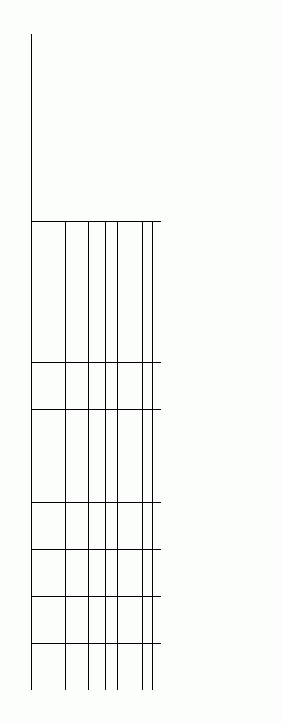
\includegraphics[width=0.16\textwidth]{grid.png}
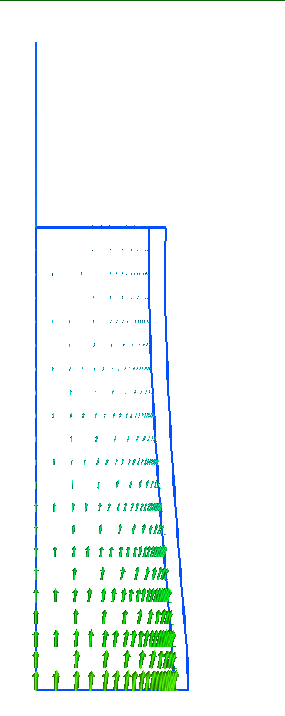
\includegraphics[width=0.16\textwidth]{t10.png}
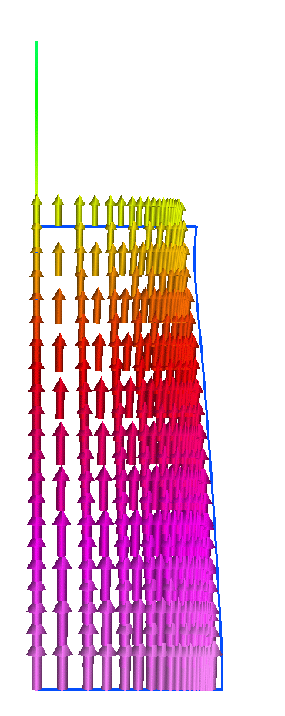
\includegraphics[width=0.16\textwidth]{t20.png}
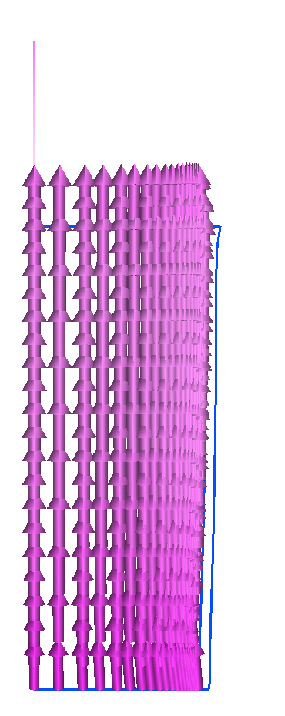
\includegraphics[width=0.16\textwidth]{t30.png}
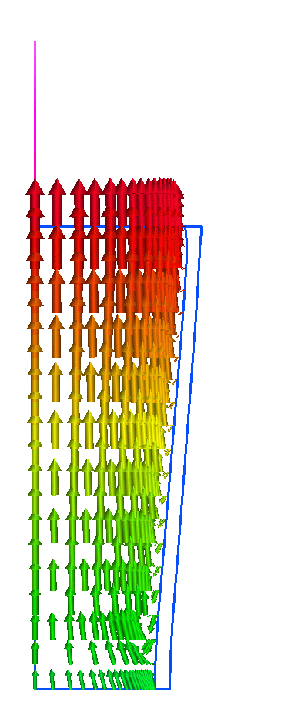
\includegraphics[width=0.16\textwidth]{t40.png}
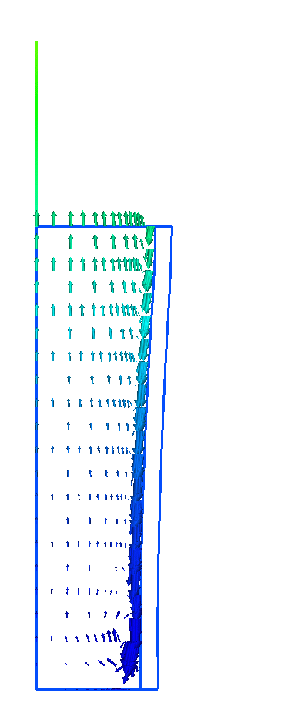
\includegraphics[width=0.16\textwidth]{t50.png}
\end{center}
\caption{An example of the model results: pressure pulse prapagation in a 2D axisymmetric 
model combined with an 1D model.}
\end{figure}

\bibliography{elmerbib}
\bibliographystyle{plain}




% Force computation
\graphicspath{{./}{fluidicforce/}}
\Chapter{Fluidic Force}

\modinfo{Module name}{\Idx{FluidicForce}}
\modinfo{Module subroutines}{ForceCompute}
\begin{versiona}
\modinfo{Module authors}{Juha Ruokolainen, Antti Pursula}
\modinfo{Document authors}{Antti Pursula}
\modinfo{Document edited}{Feb 28th 2005}


\section{Introduction}

This module is used to calculate the force that a fluid flow induces
on a surface. The fluidic force can be divided into two main
components: force due to pressure and viscous drag force. The fluid
can be compressible or incompressible and also non-Newtonian with the
same limitations than there are in the Elmer Navier-Stokes Equation
solver. The force calculation is based on a flow solution (velocity
components and pressure) which has to present when calling the
procedure. Also the torque with respect to a given point can be
requested.


\section{Theory}

The force due to fluid is calculated as a product of the stress
tensor and normal vector integrated over the surface
\begin{equation}
\vec F = \int_S \overline{\overline\sigma}\cdot\vec n~dS.
\end{equation}
The stress tensor is
\begin{eqnarray}
\overline{\overline\sigma} = 2\mu \overline{\overline\varepsilon}
-\frac{2}{3} \mu (\nabla\cdot\vec u)\overline{\overline I} - p 
\overline{\overline I},
\end{eqnarray}
where $\mu$ is the viscosity, $\vec{u}$ is the velocity, $p$ is the
pressure, $\overline{\overline I}$ the unit tensor and
$\overline{\overline \varepsilon}$ the linearized strain rate tensor,
i.e.
\begin{eqnarray}
\varepsilon_{ij} = \frac{1}{2}\left( \frac{\partial u_i}{\partial x_j} +
\frac{\partial u_j}{\partial x_i}
\right).
\end{eqnarray}
The torque about a point $\vec a$ is given by 
\begin{equation}
\vec \tau = (\vec r-\vec a)\times\vec F(\vec r),
\end{equation}
where $\vec r$ is the position vector.


\section{Additional output}

There is also a feature for saving the tangential component of the
surface force i.e. the shear stress elementwise on the boundaries. The
shear stress output is written on disk in a file which contains three
columns: 1) the value of the shear stress, 2 and 3) the corresponding
$x$ and $y$ coordinates.
The shear stress is saved on all boundaries where fluidic force
computation is requested. This feature is implemented only for
1D-boundaries of 2D-geometries.


\section{Keywords}
\end{versiona}

\sifbegin
\sifitemnt{Solver}{solver id}
\sifbegin
\sifitemnt{Equation}{String Fluidic Force}
\sifitemnt{Procedure}{File "FluidicForce"\ "ForceCompute"}
\sifitem{Calculate Viscous Force}{Logical [True]}
Setting this flag to false disables the viscous drag force, and only
the surface integral of pressure is calculated.
\sifitem{Sum Forces}{Logical [False]}
By default the solver calculates the fluidic force by
boundaries. Setting this flag to True apllies summing of each
individual boundary force in to a resultant force which is the only
force vector in output.
\sifitem{Shear Stress Output}{Logical [False]}
Setting this flag to True activates writing shear stress values on
disk.
\sifitem{Shear Stress Output File}{String [shearstress.dat]}
Defines the name of the shear stress file.
\sifitem{Velocity Field Name}{String}
The name of the velocity field variable. This keyword may be necessary
if some other flow solver than the built-in Navier-Stokes solver of
Elmer is used. Normally this keyword should be omitted.
\sifend

\sifitemnt{Material}{mat id}
\sifbegin
\sifitemnt{Viscosity}{Real}
\sifend

\sifitemnt{Boundary Condition}{bc id}
\sifbegin
\sifitem{Calculate Fluidic Force}{Logical [True]}
The fluidic force is calculated for the surfaces where 
this flag is set to true.
\sifitem{Moment About 1,2,3}{Real}
Coordinates for the point on which the torque is returned.
\sifend
\sifend




\graphicspath{{./}{electricforce/}}
\chapter{Static Electric Force}
\noindent
\modinfo{Module name}{\Idx{ElectricForce}}
\modinfo{Module subroutines}{\Idx{StatElecForce}}
\modinfo{Module authors}{Antti Pursula}
\modinfo{Document authors}{Antti Pursula}
\modinfo{Document edited}{February 7th 2003}


\section{Introduction}

This solver calculates the electrostatic force acting on a
surface. The calculation is based on an electrostatic potential which
can be solved by the electrostatic solver (see Model~\ref{Electrostatics}
of this Manual).


\section{Theory}

The force is calculated by integrating the electrostatic \Idx{Maxwell
stress tensor}~\cite{vanderlinde93} over the specified surface. Using
the stress tensor $\overline{\overline T}$ the total force on the
surface $S$ can be expressed as
\begin{equation}
\Vec{F} = \int_S \overline{\overline T}\cdot~d\Vec{S}.
\end{equation}
The components of the Maxwell stress tensor for linear medium are
\begin{equation}
T_{ij} = -D_iE_j + \frac{1}{2}\delta_{ij}\Vec{D}\cdot\Vec{E},
\end{equation}
where electric field $\vec{E}$ and electric displacement field
$\vec{D}$ are obtained from the electric potential $\Phi$
\begin{equation}
\vec{E} = -\nabla\Phi,
\end{equation}
and
\begin{equation}
\vec{D} = -\varepsilon_0\varepsilon_r\nabla\Phi,
\end{equation}
where $\varepsilon_0$ is the permittivity of vacuum and
$\varepsilon_r$ is the relative permittivity of the material, which
can be a tensor.


\section{Keywords}

\sifbegin
\sifitemnt{Constants}{}
\sifbegin
\sifitemnt{Permittivity Of Vacuum}{Real [8.8542e-12]}
\sifend

\sifitemnt{Solver}{solver id} 
\sifbegin
\sifitem{Equation}{String Electric Force}
The name of the equation. Not necessary.
\sifitemnt{Procedure}{File "ElectricForce"\ "StatElecForce"}
\sifitem{Exec Solver}{String After Timestep}
Often it is not necessary to calculate force 
until solution is converged.
\sifend

\sifitemnt{Material}{mat id}
\sifbegin
\sifitemnt{Relative Permittivity}{Real}
\sifend

\sifitemnt{Boundary Condition}{bc id}
\sifbegin
\sifitem{Calculate Electric Force}{Logical True}
This keyword marks the boundaries where
force is calculated.
\sifend

\sifend

\bibliography{elmerbib}
\bibliographystyle{plain}



\graphicspath{{./}{savedata/}}
\Chapter{Save Data}

\noindent
\modinfo{Module name}{\Idx{SaveData}}
\modinfo{Module subroutines}{\Idx{SaveScalars}, \Idx{SaveLine}, \Idx{SaveMaterials}, \Idx{SaveBoundaryValues}}
\begin{versiona}
\modinfo{Module authors}{Peter R�back, Ville Savolainen, Thomas Zwinger}
\modinfo{Document authors}{Peter R�back}
\modinfo{Document created}{Oct 3rd 2002}
\modinfo{Document updated}{January 8th 2008}

\section{Introduction}

This module does not include any physical models per se.
The module includes utilities for computing derived quantities and 
saving scalars as well as  
lines in matrix format. Scalars are saved with the subroutine 
\texttt{SaveScalars} and lines with the subroutine 
\texttt{SaveLine}, correspondingly.
The results are easily 
then utilized by MatLab, Excel or any other program that can 
read ASCII data. In addition to the number values also
an additional file with the suffix \texttt{.name} is saved. 
It tells what variables are at each column.
In addition there is a utility called \texttt{SaveMaterials} 
that may be used to create additional
field variables from the material parameters. A similar procedure \texttt{SaveBoundaryValues} stores parameters defined on boundaries as variables for the whole mesh. This can be of help if a boundary condition that is not directly accessible from the variables (like a normal component of a vector field) should be evaluated in the post-processing step.

\section{Theory}

The theoretical problem in saving data comes from the fact that
often the data should be saved in points or lines that were not 
a priori defined. 

If there are relatively few points the dummy algorithm
where each element is checked for including the 
node may be used. For the lines, however, this algorithm
might become quite expensive as there may be many points
that constitute the line. Therefore we only look for intersections
of element faces and the lines. Each element face is divided into triangles.
The triangle has points $\vec{e}_1$, $\vec{e}_2$ and $\vec{e}_3$. The
line is drawn between points $\vec{r}_1$ and $\vec{r}_2$.
Therefore the line goes through the point only if
\begin{equation}
   \vec{r}_1 + a (\vec{r}_2 - \vec{r}_1) = 
\vec{e}_1 + b (\vec{e}_2 - \vec{e}_1) +  c (\vec{e}_3 - \vec{e}_1)
\end{equation}
has a solution for which $0\le a, b, c \le 1$. This 
results to a matrix equation
\begin{equation}
\begin{pmatrix}
r_{2x} - r_{1x} & e_{1x}-e_{2x} & e_{1x}-e_{3x} \\
r_{2y} - r_{1y} & e_{1y}-e_{2y} & e_{1y}-e_{3y} \\
r_{2z} - r_{1z} & e_{1z}-e_{2z} & e_{1z}-e_{3z}
\end{pmatrix}
\begin{pmatrix}
a \\
b \\
c 
\end{pmatrix}
=
\begin{pmatrix}
e_{1x} - r_{1x} \\
e_{1y} - r_{1y} \\
e_{1z} - r_{1z} 
\end{pmatrix}
\end{equation}
which may be easily solved with standard methods linear algebra.
Because the face element is a triangle there is an additional 
condition that $b+c \le 1$.

When saving statistical information there are two possibilities. We may use normal number statistics
where each node is given an equal weight. Then, for example the mean becomes,
\begin{equation}
  <f> = \frac{\sum_{i=1}^n f_i}{n}.
\end{equation}
The other possibility is to treat the variable as a continuous function and 
compute the statistical values as averages over the domain. Now the 
mean is 
\begin{equation}
  <f> = \frac{\int f \, d\Omega}{\int d\Omega}.
\end{equation}
In addition to the mean we may compute the mean
deviation, $<|f-<f>|>$.and 
the variance
  $\delta f = \sqrt{ <f^2> - <f>^2} $.

It is possible to compute energy type of lumped quantities
by integrating over the domain. The energy of the field $f$ resulting 
from a diffusion equation is 
\begin{equation}
  E_{diff} = \frac{1}{2} \int_\Omega \nabla f \cdot c \nabla f \, d\Omega,
\end{equation}
where $c$ may a tensor or a scalar.
 Kinetic energy related to convection is of type
\begin{equation}
  E_{con} = \frac{1}{2} \int_\Omega c \vec{v} \cdot \vec{v}  \, d\Omega,
\end{equation}
and potential type of energy
\begin{equation}
  E_{pot} = \int_\Omega c f \, d\Omega.
\end{equation}

Sometimes it may be interesting to compute the fluxes through surfaces.
The values may be used in evaluating the accuracy of the results --
what goes in should in steady state also come out. 
There are two different fluxes that may be
computed. For convective field the flux is of type
\begin{equation}
  F_{con} = \int_\Gamma c \vec{v} \cdot \vec{n} \, d\Gamma, 
\end{equation}
where $\vec{n}$ is the surface normal. Diffusive fluxes may be computed from
\begin{equation}
  F_{diff} = \int_\Gamma c \nabla f \cdot \vec{n} \, d\Gamma , 
\end{equation}
where $c$ may also be a tensor.


\section{Keywords}
\end{versiona}

\subsection*{Keywords of solver SaveScalars}

\sifbegin
\sifitemnt{Solver}{solver id}
\sifbegin
\sifitemnt{Procedure}{File "SaveData"\ "SaveScalars"}
\sifitem{Filename}{String}
Name of the file where results are to be saved, the default is {\tt scalars.dat}.
\sifitem{Scalars Prefix}{String}
Save constants starting with this prefix. The default is {\tt res:}.
\sifitem{Variable i}{String}
The names of the variables to be saved. There can be up to 
99 variables. In addition to field variables there are some special variables.
The scalar variables. e.g. \texttt{Time}, are saved as is. There are also
variables \texttt{CPU Time} and \texttt{CPU Memory} that may be used to save 
execution details.  
%
\sifitem{Save Points}{Size n Integer}
Save the specified degrees of freedom in the $n$ nodes specified.
%
\sifitem{Save Coordinates}{Size n DIM Real}
Save the degrees of freedom in the nodes nearest 
to the given $n$ coordinates.
%
\sifitem{Exact Coordinates}{Logical}
When this keyword is true the coordinates will be looked in an exact manner.
Then the degrees of freedom are linear combinations of the node values 
of the element that the point belongs to.
%
\sifitem{Moving Mesh}{Logical}
If this parameter is \texttt{True} the saved points will be defined every time the subroutine
is visited. The default is \texttt{False}.
\sifitem{File Append}{Logical}
If the results from consecutive rounds should be appended to the file
this flag should be set to \texttt{True}. The default is {\tt False}.
%
\sifitem{Operator i}{String}
There are different operators that may be performed on all the
given variables. These include operators working on the set of numbers, 
\texttt{max, min, max abs, min abs, mean, variance} and \texttt{deviation}.
There are also a few operators that use statistics over the volume,
\texttt{int mean} and \texttt{int variance}.
The volume used by a given variable is obtained by
operator \texttt{volume}. If a name for the coefficient, is given for the 
operator, the integral is taken over the coefficient. One can for example
obtain the weight from a integral over \texttt{Density}.

There are also a number of similar operators that only operate on the boundary.
These are invoked by \texttt{boundary sum}, \texttt{boundary dofs}, \texttt{boundary mean},
\texttt{boundary max}, \texttt{boundary min}, 
\texttt{boundary max abs}, and \texttt{boundary min abs}.

Three different energy type of quantities may be computed by 
\Idx{domain integral} operators
\texttt{diffusive energy, convective energy, potential energy}. 
Finally, also \Idx{boundary integral}s are possible using operators
\texttt{diffusive flux}, \texttt{convective flux} and \texttt{area}. 
These require that in the boundary conditions 
the active boundaries are defined. Also here there may be an optional 
coefficient.

Some operators do not work on the solution itself but use other info related to that.
Operator \texttt{dofs} simply returns the length of 
the variable under study. Operator \texttt{norm} returns the last computed norm of the 
field variable, and operators \texttt{nonlinear change} and \texttt{steady state change} return
the last computed convergence measures at the nonlinear and steady state levels. 

There may be up to 99 different operators.
If the variable is a vector the statistics is performed on its length.
%
\sifitem{Coefficient i}{String}
Even though only limited number of operators are given 
almost any energy or flux kind of quantity may be computed since 
the coefficient $c$ may be defined by the user.
The idea is that the same data that is already used as a material
parameter can be simple referred to by its name.
The coefficient may be,
\texttt{Heat Conductivity}, \texttt{Permittivity}, \texttt{Density}, 
for example. Usually the coefficient is the same that was used in computing
the field variable under integration.
For the \texttt{diffusive energy} and \texttt{diffusive flux} 
the coefficient may even be a matrix. 
This parameter is optional and the default is one.
%
\sifitem{Polyline Coordinates}{Size n DIM}
This keyword may be used to create line segments that are defined by
points $x_1$, $y_1$, $x_2$, and $y_2$. For each line different
kinds of fluxes trough the elements may be computed.
This makes it possible, for example, to check the mass flux 
even though no boundary has a priori been defined.  
\sifend

\sifitemnt{Boundary Condition}{bc id}
\sifbegin
\sifitem{Save Scalars}{Logical}
The flag activates the computation of boundary related information.
The results are treated independently for each boundary.
The keyword replaces the previously used \texttt{Flux Integrate}. 
\sifend
\sifend



\subsection*{Keywords of subroutine SaveLine}

\sifbegin
\sifitemnt{Solver}{solver id}
\sifbegin
\sifitemnt{Procedure}{File "SaveData"\ "SaveLine"}
\sifitem{Filename}{String}
Name of the file where results are to be saved, the default is 
{\tt sides.dat}. 
\sifitem{File Append}{Logical}
If the results from consecutive rounds should be appended to the file
this flag should be set to {\tt True}. The default is {\tt False}.

\sifitem{Save Axis}{Logical}
Save all the principal axis. Also keywords {\tt Save Axis i} exist, where
{\tt i}=1,2,3 defines the axis. 
%
\sifitem{Polyline Coordinates}{Size n DIM}
Save the line consisting of line sections defined by two points. 
There can be more than one set of points but as a line segment is 
defined by two points there must be an even number of points.
%
\sifitem{Variable i}{String} 
By default \texttt{SaveLine} saves all the active variables. However, it is possible to
save only a specified list of variables given by this keyword where {tt i}=1,2,3,\ldots
This may be particularly useful if one wants to save a table of linear dependece, for example 
Temperature along $x$-direction, to be used as a boundary condition in consecutive Elmer runs
with a different mesh.


\sifitem{Save Flux}{Logical}
Saves a flux resulting from a gradient of a field by the model
$h=-\kappa \partial T/\partial n$. This may only be applied 
to existing boundaries, not lines defined by points.
%
\sifitem{Flux Variable}{String}
The name of the field variable (default $T$ is {\tt Temperature}).
\sifitem{Flux Coefficient}{String}
The diffusion constant (by default $\kappa$ is {\tt Heat Conductivity})

\sifitem{Save Mask}{String}a
By default SaveLine saves only the values that are on boundary marked with 
\texttt{Save Line} flag. If the user wants several instances of the SaveLine subroutine,
for saving different buondaries to different files, the mask name may be defined by this keyword.
The correspondingly one should use the same flag in the \texttt{Boundary Condition} and 
{Body} section.


\sifend

\sifitemnt{Boundary Condition}{bc id}
\sifbegin
\sifitem{Save Line}{Logical}
The flag activates the saving of the boundary condition as a line.
The subroutine tries to save the finite-element lines as a chain of points
to enable nice preprocessing with MatLab or similar tools.
The flux may only be saved on lines defined by boundary conditions.
\sifend
\sifend


\subsection*{Keywords of subroutine SaveMaterials}

\sifbegin
\sifitemnt{Solver}{solver id}
\sifbegin
\sifitemnt{Procedure}{File "SaveData"\ "SaveMaterials"}
\sifitem{Parameter i}{String}
The user may choose a number of parameters (i=1,\ldots,99) which
will be save as variables. This may be particularly handy if one wants to
visualize how the parameters depend on the position over the domain. Values in bodies with the assigned material list not containing the keyword of the parameter are set to zero by default.
\sifend
\sifend

\subsection*{Keywords of subroutine SaveBoundaryValues}

\sifbegin
\sifitemnt{Solver}{solver id}
\sifbegin
\sifitemnt{Procedure}{File "SaveData"\ "SaveBoundaryValues"}
\sifitem{Variable}{String -nooutput dummyvar}
a dummy variable for the solver that does not show up
\sifitem{Variable DOFs} {Integer  1}
\sifitem{Parameter i}{String}
The user may choose a number of parameters (i=1,\ldots,99) which
will be save as variables. These parameters will then be stored as variables with the values assigned as they were found on the specific boundary. Bulk values and values on boundaries with the parameter not being defined are set to zero by default.
\sifend
\sifend


\graphicspath{{./}{reloadinput/}}
\chapter{Runtime Control of the Solver}

\noindent
\modinfo{Module name}{\Idx{ReloadInput}}
\modinfo{Module subroutines}{ReloadInput}
\modinfo{Module authors}{Juha Ruokolainen}
\modinfo{Document authors}{Peter R�back}
\modinfo{Document created}{Februrary 5th 2003}

\section{Introduction}

This subroutine is intended for cases where the user wants
to have \Idx{run-time control} over the solution. 
The control is obtained by reloading the command file
(.sif-file) during the solution. This is done with on
additional solver that is called similarly as any other solver 
during the solution process. 

The most likealy usage of the solver is in cases where the 
user realizes during the solution process that the some 
parameters were not optimally chosen. For example, the 
convergence critaria may have been set too tight for optimal
performance. Then the user may set looser criteria by editing the 
command file during the computation. Once the new value is read 
the solver will apply the new criteria thereafter.

\section{Limitations}
The solver should not be used for things that need allocation. 
For example, the number of solvers or boundaries may not change.
Also the computational mesh must remain the same. 


\section{Keywords}

\sifbegin
\sifitemnt{Solver}{solver id}
\sifbegin
\sifitem{Equation}{String "Reload"}
The name of the equation. This is actually not much needed 
since there are no degrees of freedom associated with this solver.
\sifitem{Procedure}{File "ReloadInput"\ "ReloadInput"}
The name of the file and subroutine. 
\sifend
\sifend



%%%%%%%%%%%%%%%%%%%%%%%%%%%%%%%%%%%%%%%%%%%%%%%%%%%%%%%%%%%%

% Include the index
\printindex

%%%%%%%%%%%%%%%%%%%%%%%%%%%%%%%%%%%%%%%%%%%%%%%%%%%%%%%%%%%%

\end{document}

%%%%%%%%%%%%%%%%%%%%%%%%%%%%%%%%%%%%%%%%%%%%%%%%%%%%%%%%%%%%

